\subsection{External Interface Requirements}
This chapter provides a detailed description of the system's external interfaces such as the User, Hardware, Software, and Communication interfaces. 
\subsubsection{User Interfaces}
The user interface will be designed to improve intuitiveness and simplicity. The platform root page is the Home Page from which every non-registered user can find information about S\&C such as the latest news. The Home page is linked to other pages, such as the Dashboard, Contacts, and About page, using an app bar. 
In the Contacts page, the user can find useful links to get in touch with S\&C.\\
\begin{figure}[H]
    \centering
    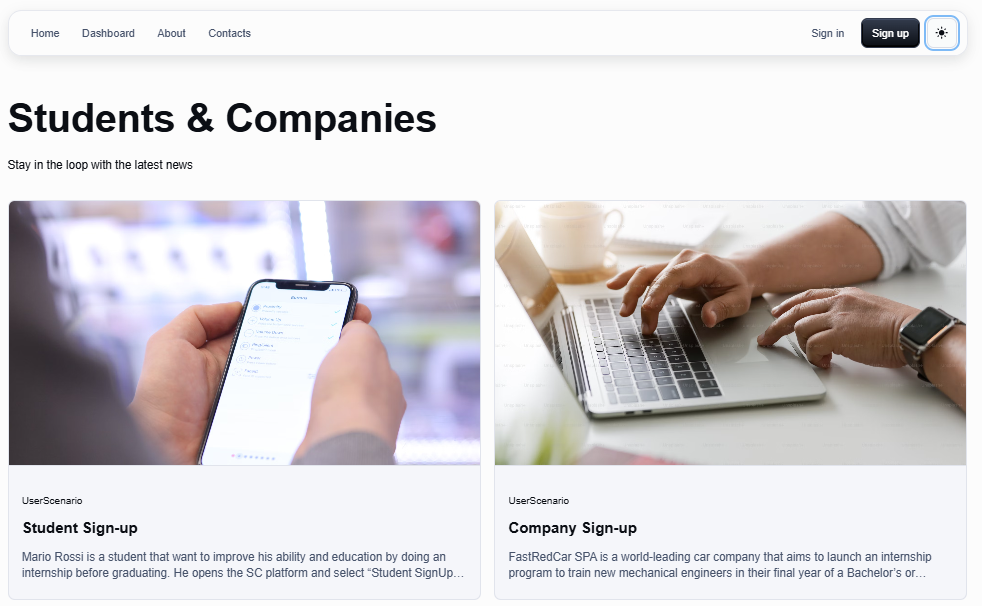
\includegraphics[width=\textwidth]{Latex/Images/HomePage.png}
    \caption{UI Home Page: as an example, UI cards containing some user scenarios described in the \ref{subsec: user scenarios}  are shown}
    \label{fig:homepage}
\end{figure}
\begin{figure}[H]
    \centering
    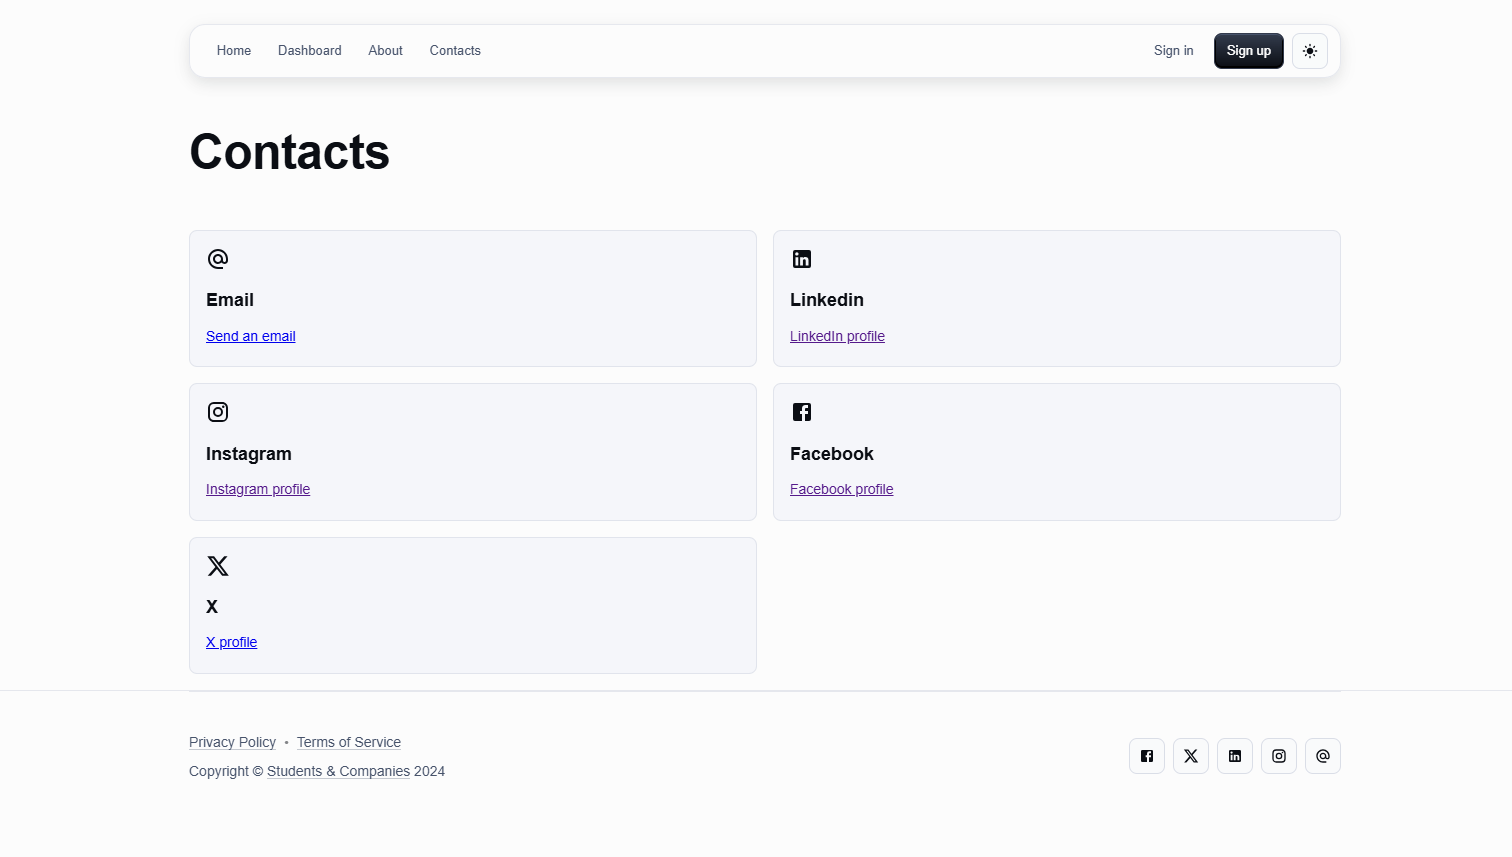
\includegraphics[width=\textwidth]{Latex/Images/New Ui/Contacts.png}
    \caption{UI Contacts Page}
    \label{fig:contactpage}
\end{figure}
\noindent Thanks to the app bar link buttons, users can also reach the Sign-Up and Sign-in pages. The Sign-Up page allows for different types of sign-up according to the new user type. This allows the user to provide the platform with the correct information.
\begin{figure}[H]
    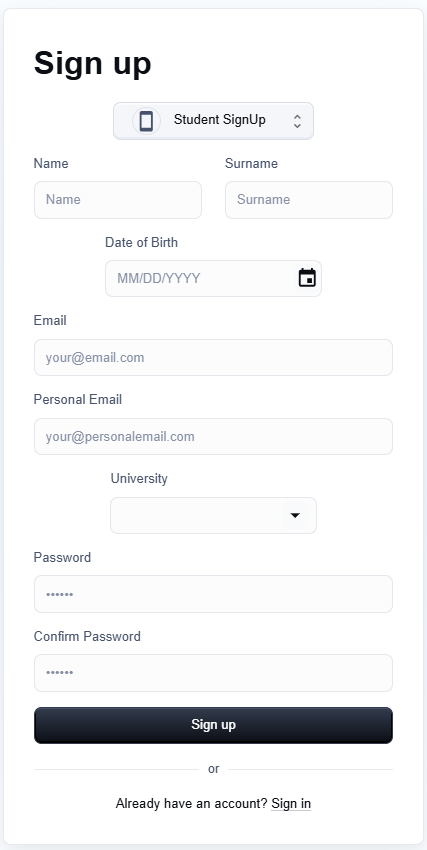
\includegraphics[width=0.33\textwidth]{Latex/Images/New Ui/SignUp Student.png}
    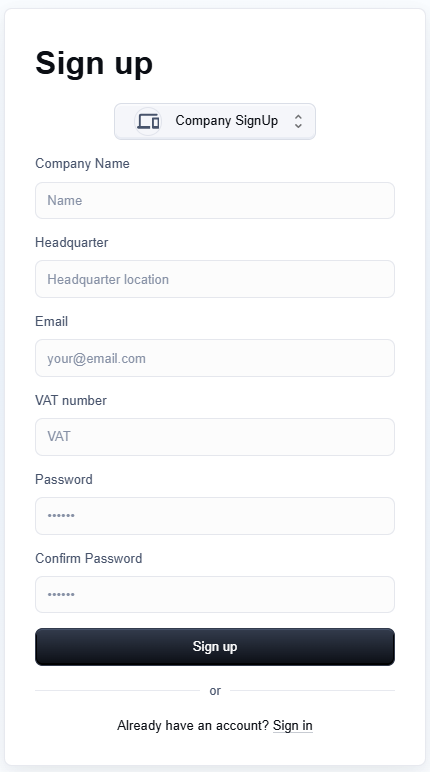
\includegraphics[width=0.33\textwidth]{Latex/Images/New Ui/SignUp Company.png}
    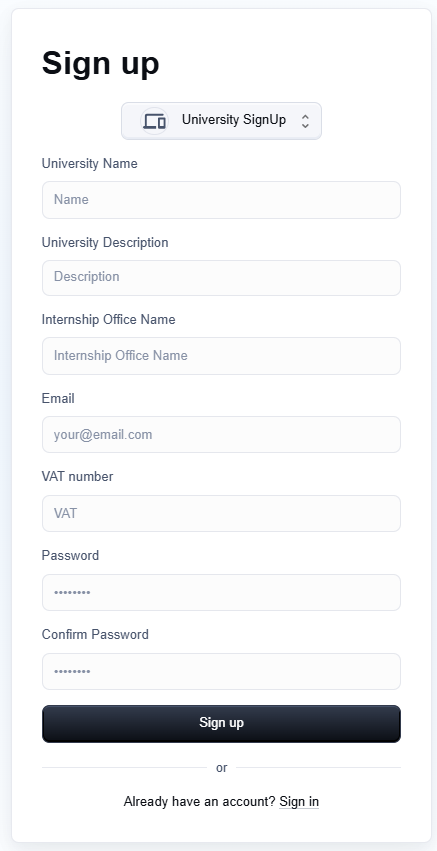
\includegraphics[width=0.33\textwidth]{Latex/Images/New Ui/SignUp University.png}
    \caption{UI Sign-Up Page}
    \label{fig:signuppage}
\end{figure}
To be able to log into the platform, the user shall provide his email and password. 
\begin{figure}[H]
    \centering
    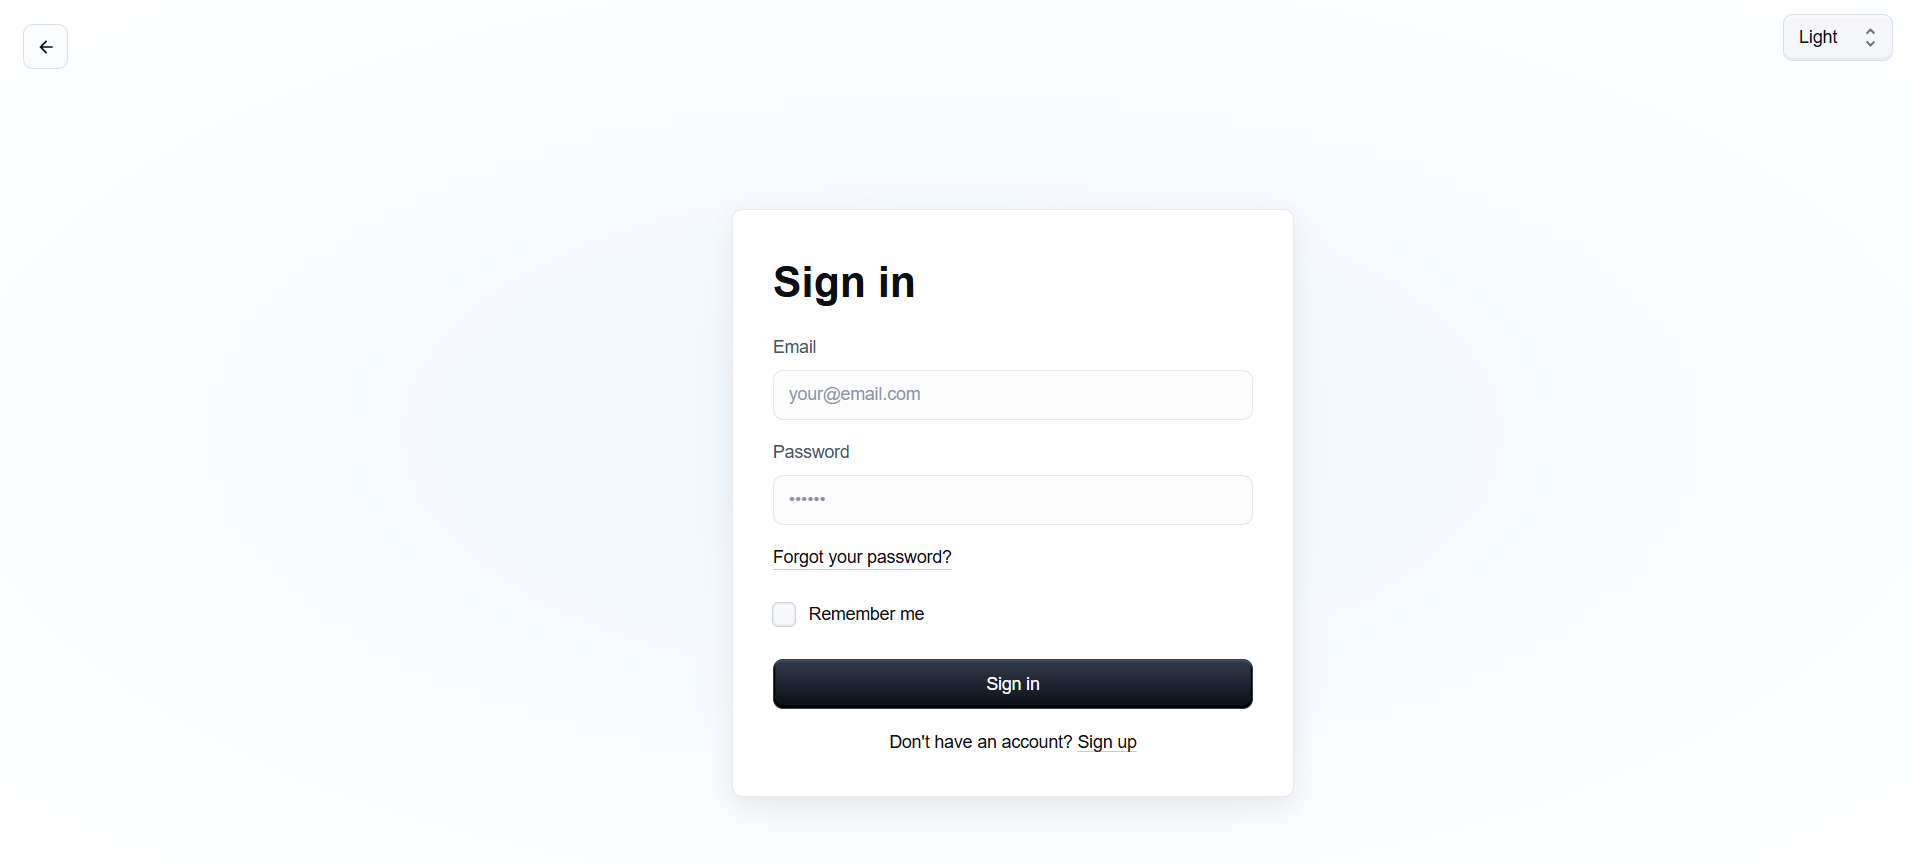
\includegraphics[width=\textwidth]{Latex/Images/New Ui/SignInPage.png}
    \caption{UI Sign-In Page}
    \label{fig:signinpage}
\end{figure}
\noindent The Dashboard page will be the central hub for logged-in users. From the left-hand panel of the dashboard, all the pages associated with the core functionalities of the platform are reachable. Therefore, this page is provided after a successful log-in. The side panel contains different elements according to the user needs.
\begin{figure}[H]
    \centering
    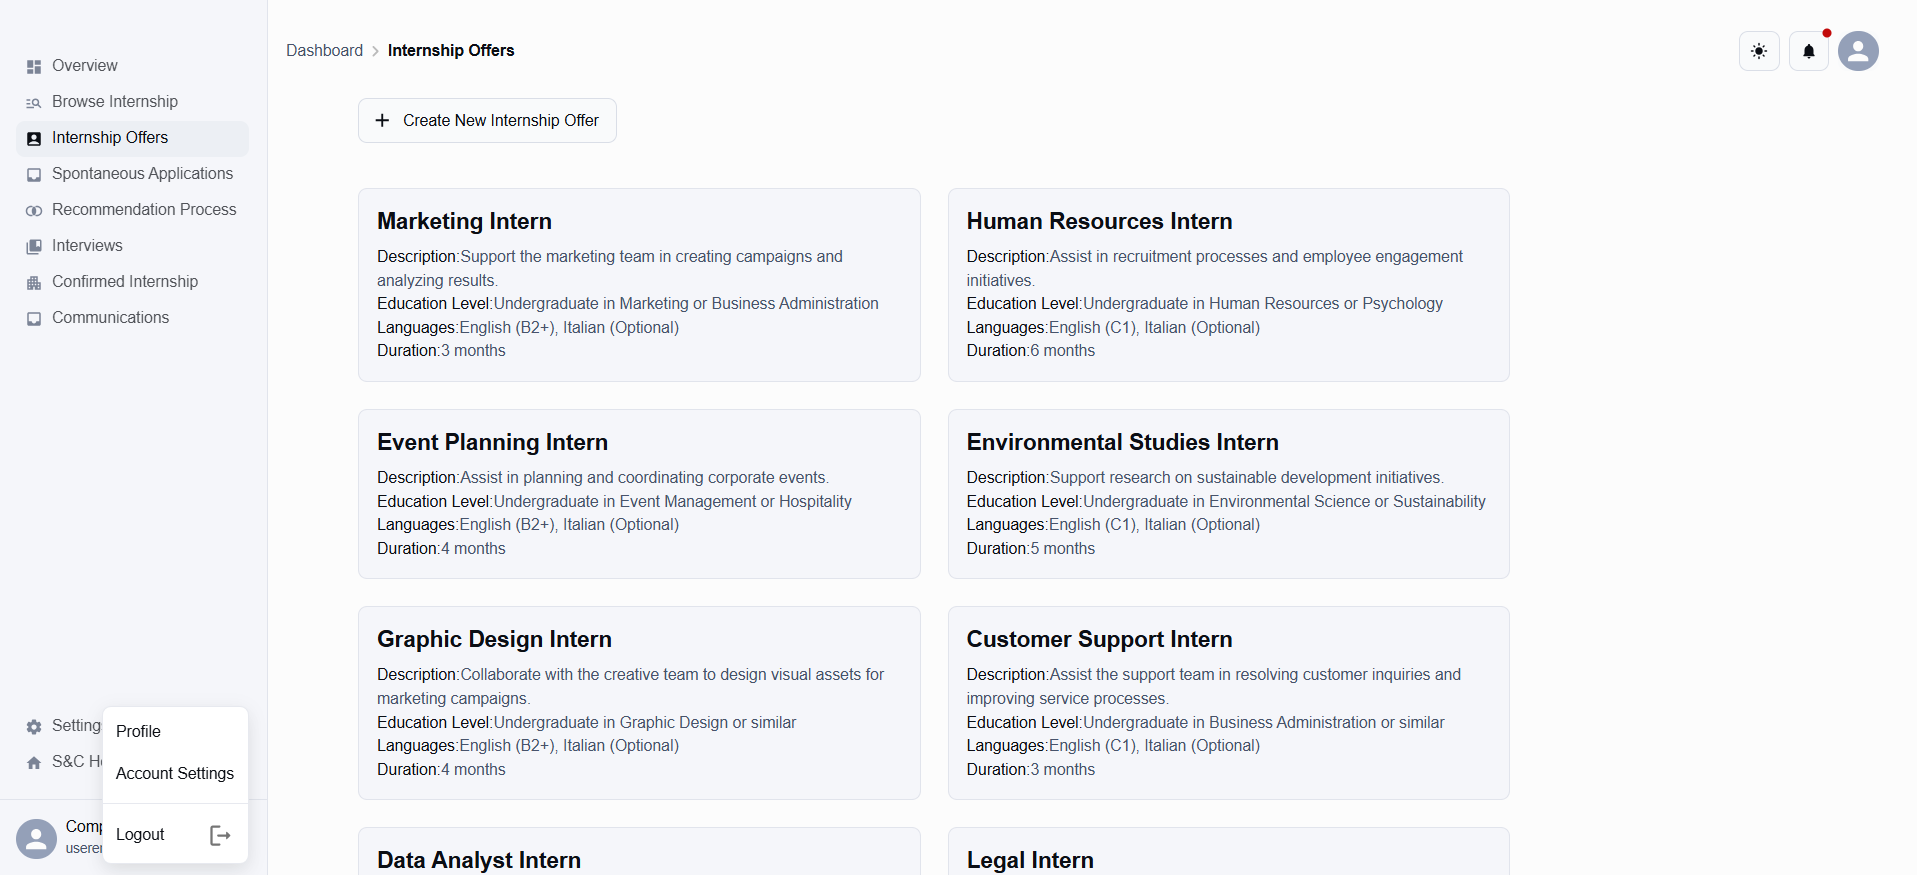
\includegraphics[width=\textwidth]{Latex/Images/New Ui/Company-Dashboard.png}
    \caption{UI Company Dashboard Page}
    \label{fig:companyDashboard}
\end{figure}
\begin{figure}[H]
    \centering
    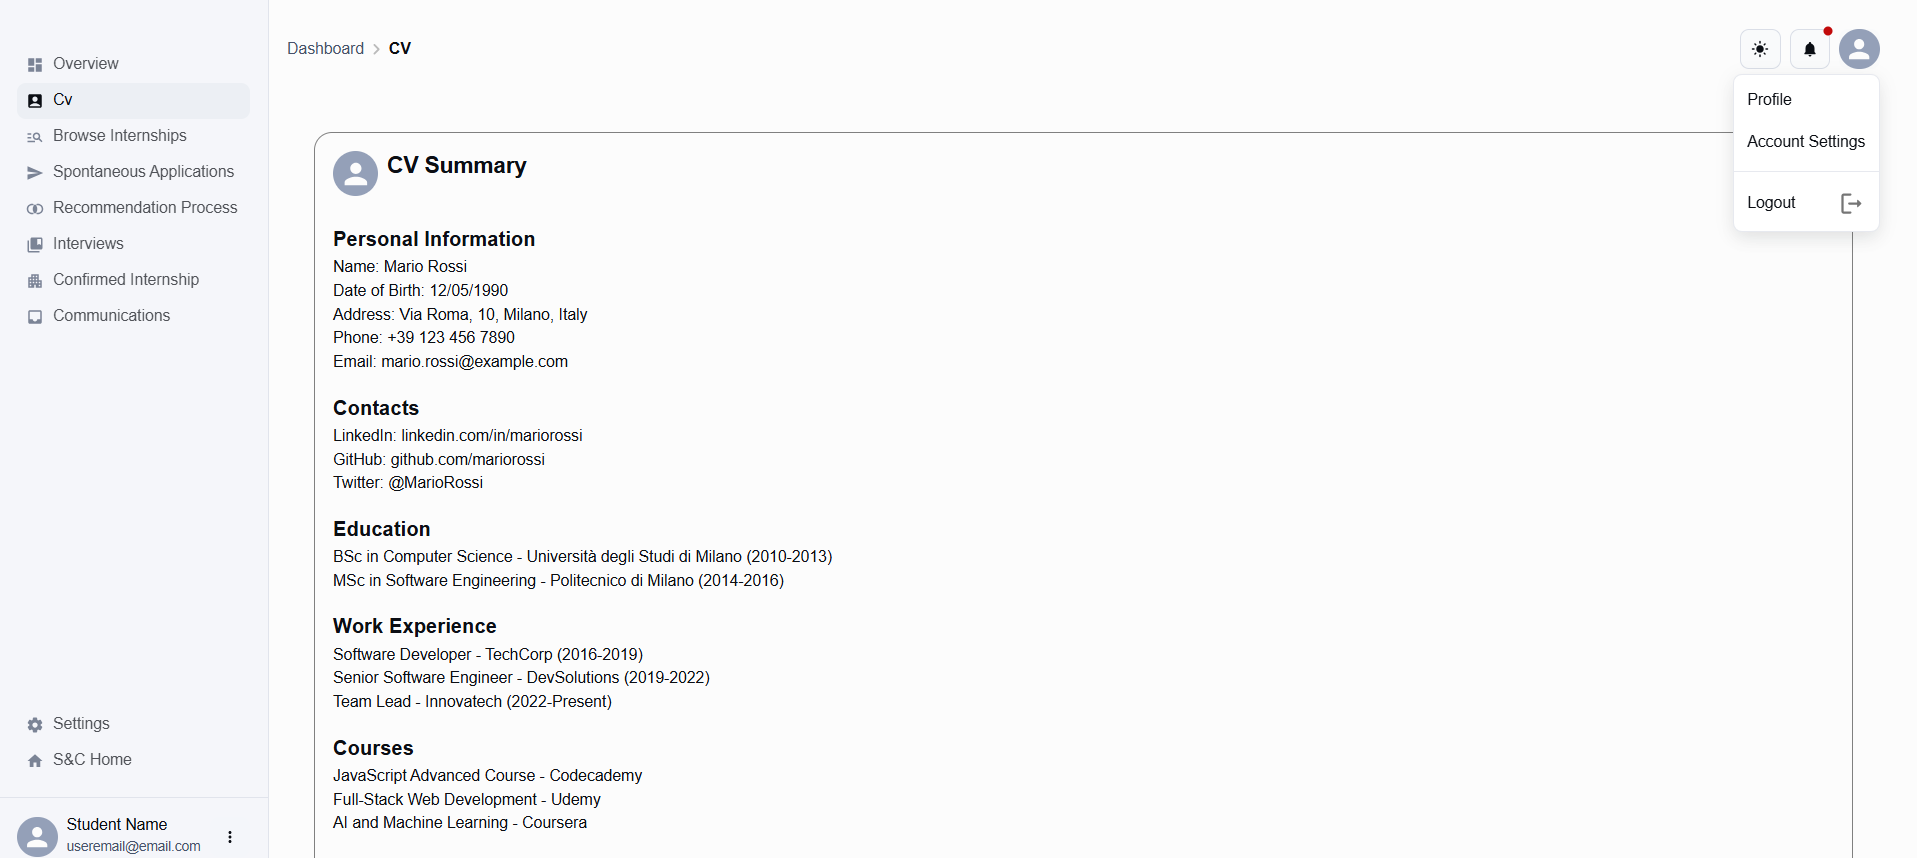
\includegraphics[width=\textwidth]{Latex/Images/New Ui/Student-Dashboard.png}
    \caption{UI Students Dashboard Page}
    \label{fig:studentDashboard}
\end{figure}
\begin{figure}[H]
    \centering
    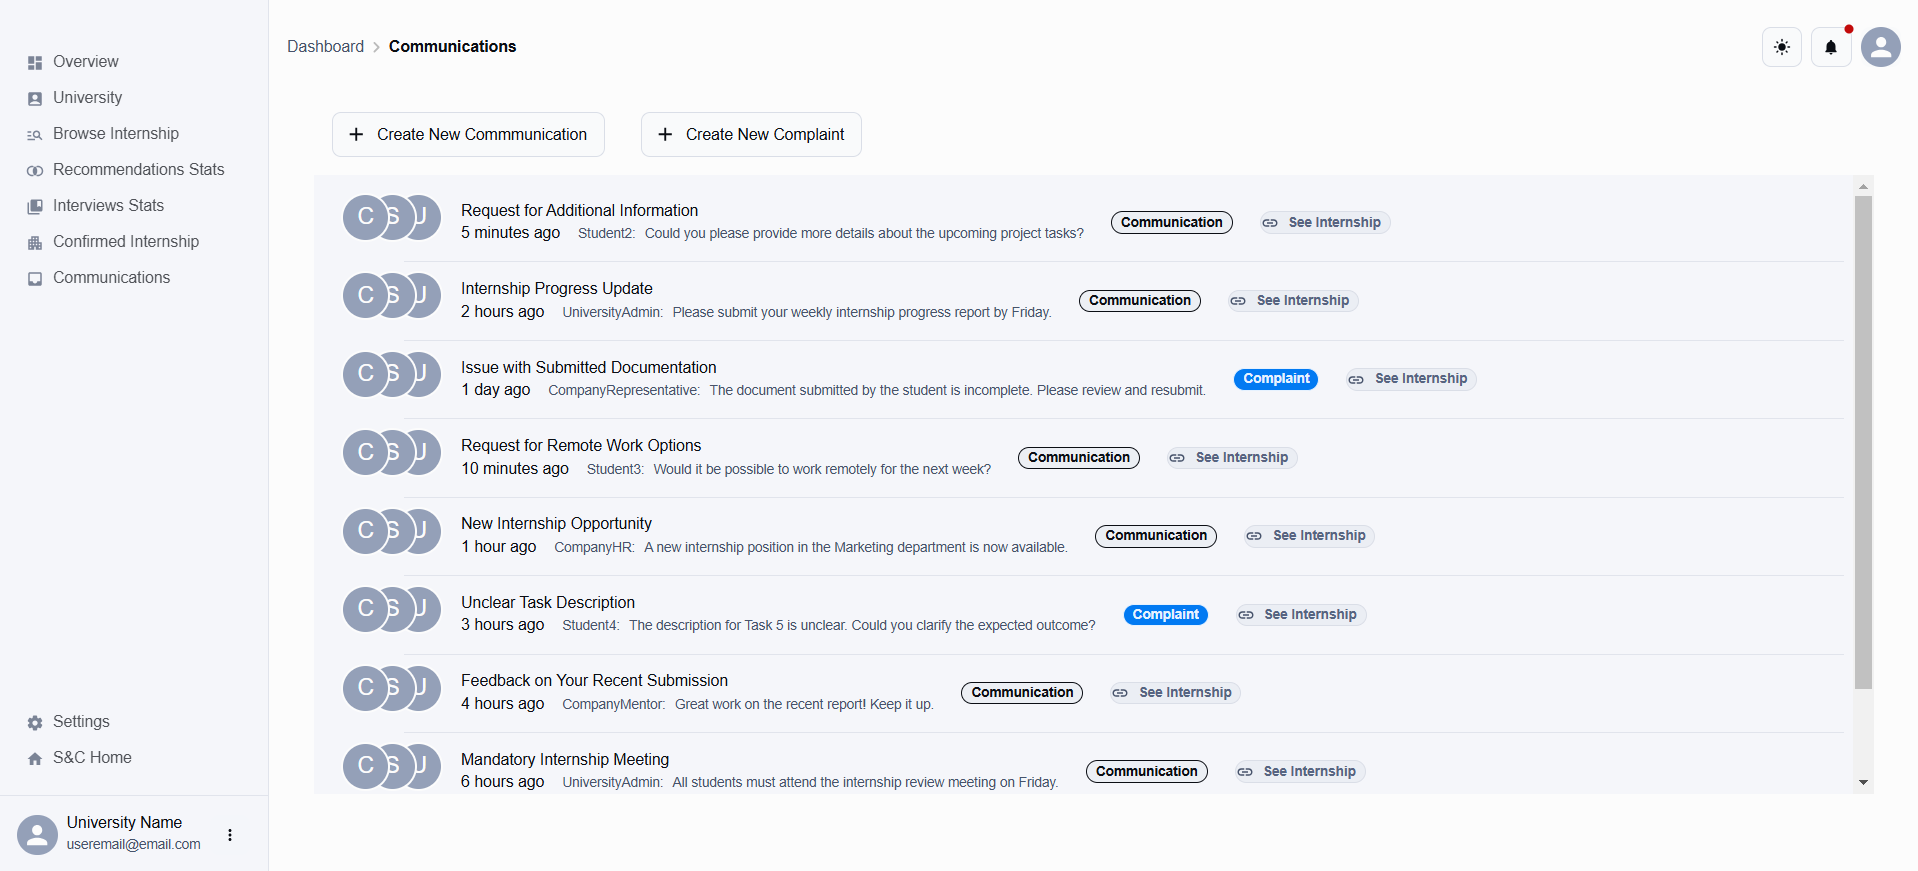
\includegraphics[width=\textwidth]{Latex/Images/New Ui/Uni-Dashboard.png}
    \caption{UI University Dashboard Page}
    \label{fig:universityDashboard}
\end{figure}

\subsubsection{Hardware Interfaces}
The platform is a web application that can be accessed from any device with a web browser and an internet connection like a PC, a tablet, or a smartphone. No specific hardware requirements are needed to interact with the Student\&Company platform.
\subsubsection{Software Interfaces}
\label{subsec:SWInteface}
An Email Provider, through its interface, is used by the Platform to send a confirmation email to Users upon registration. \\
A notification manager is used to send notification to Users when relevant events occur. Using notifications instead of email allows the platform to provide a more immediate and interactive experience to the Users without generating spam that can be seen as annoying by the Users.\\
At this stage of development, no other external software interfaces are required.
\subsubsection{Communication Interfaces}
The platform uses standard internet communication protocols to interact with Users and the backend server. At this stage of development other specific communication interfaces are not defined yet.

\subsection{Functional Requirements}
This chapter provides a comprehensive overview of the system's use cases, detailing the various interactions between Users and the system.
Use Case Diagrams, detailed Use Case Descriptions, Sequence Diagrams and Requirement Mapping are provided for each use case.
\subsubsection{Use Case Diagrams}
\begin{figure}[H]
    \centering
    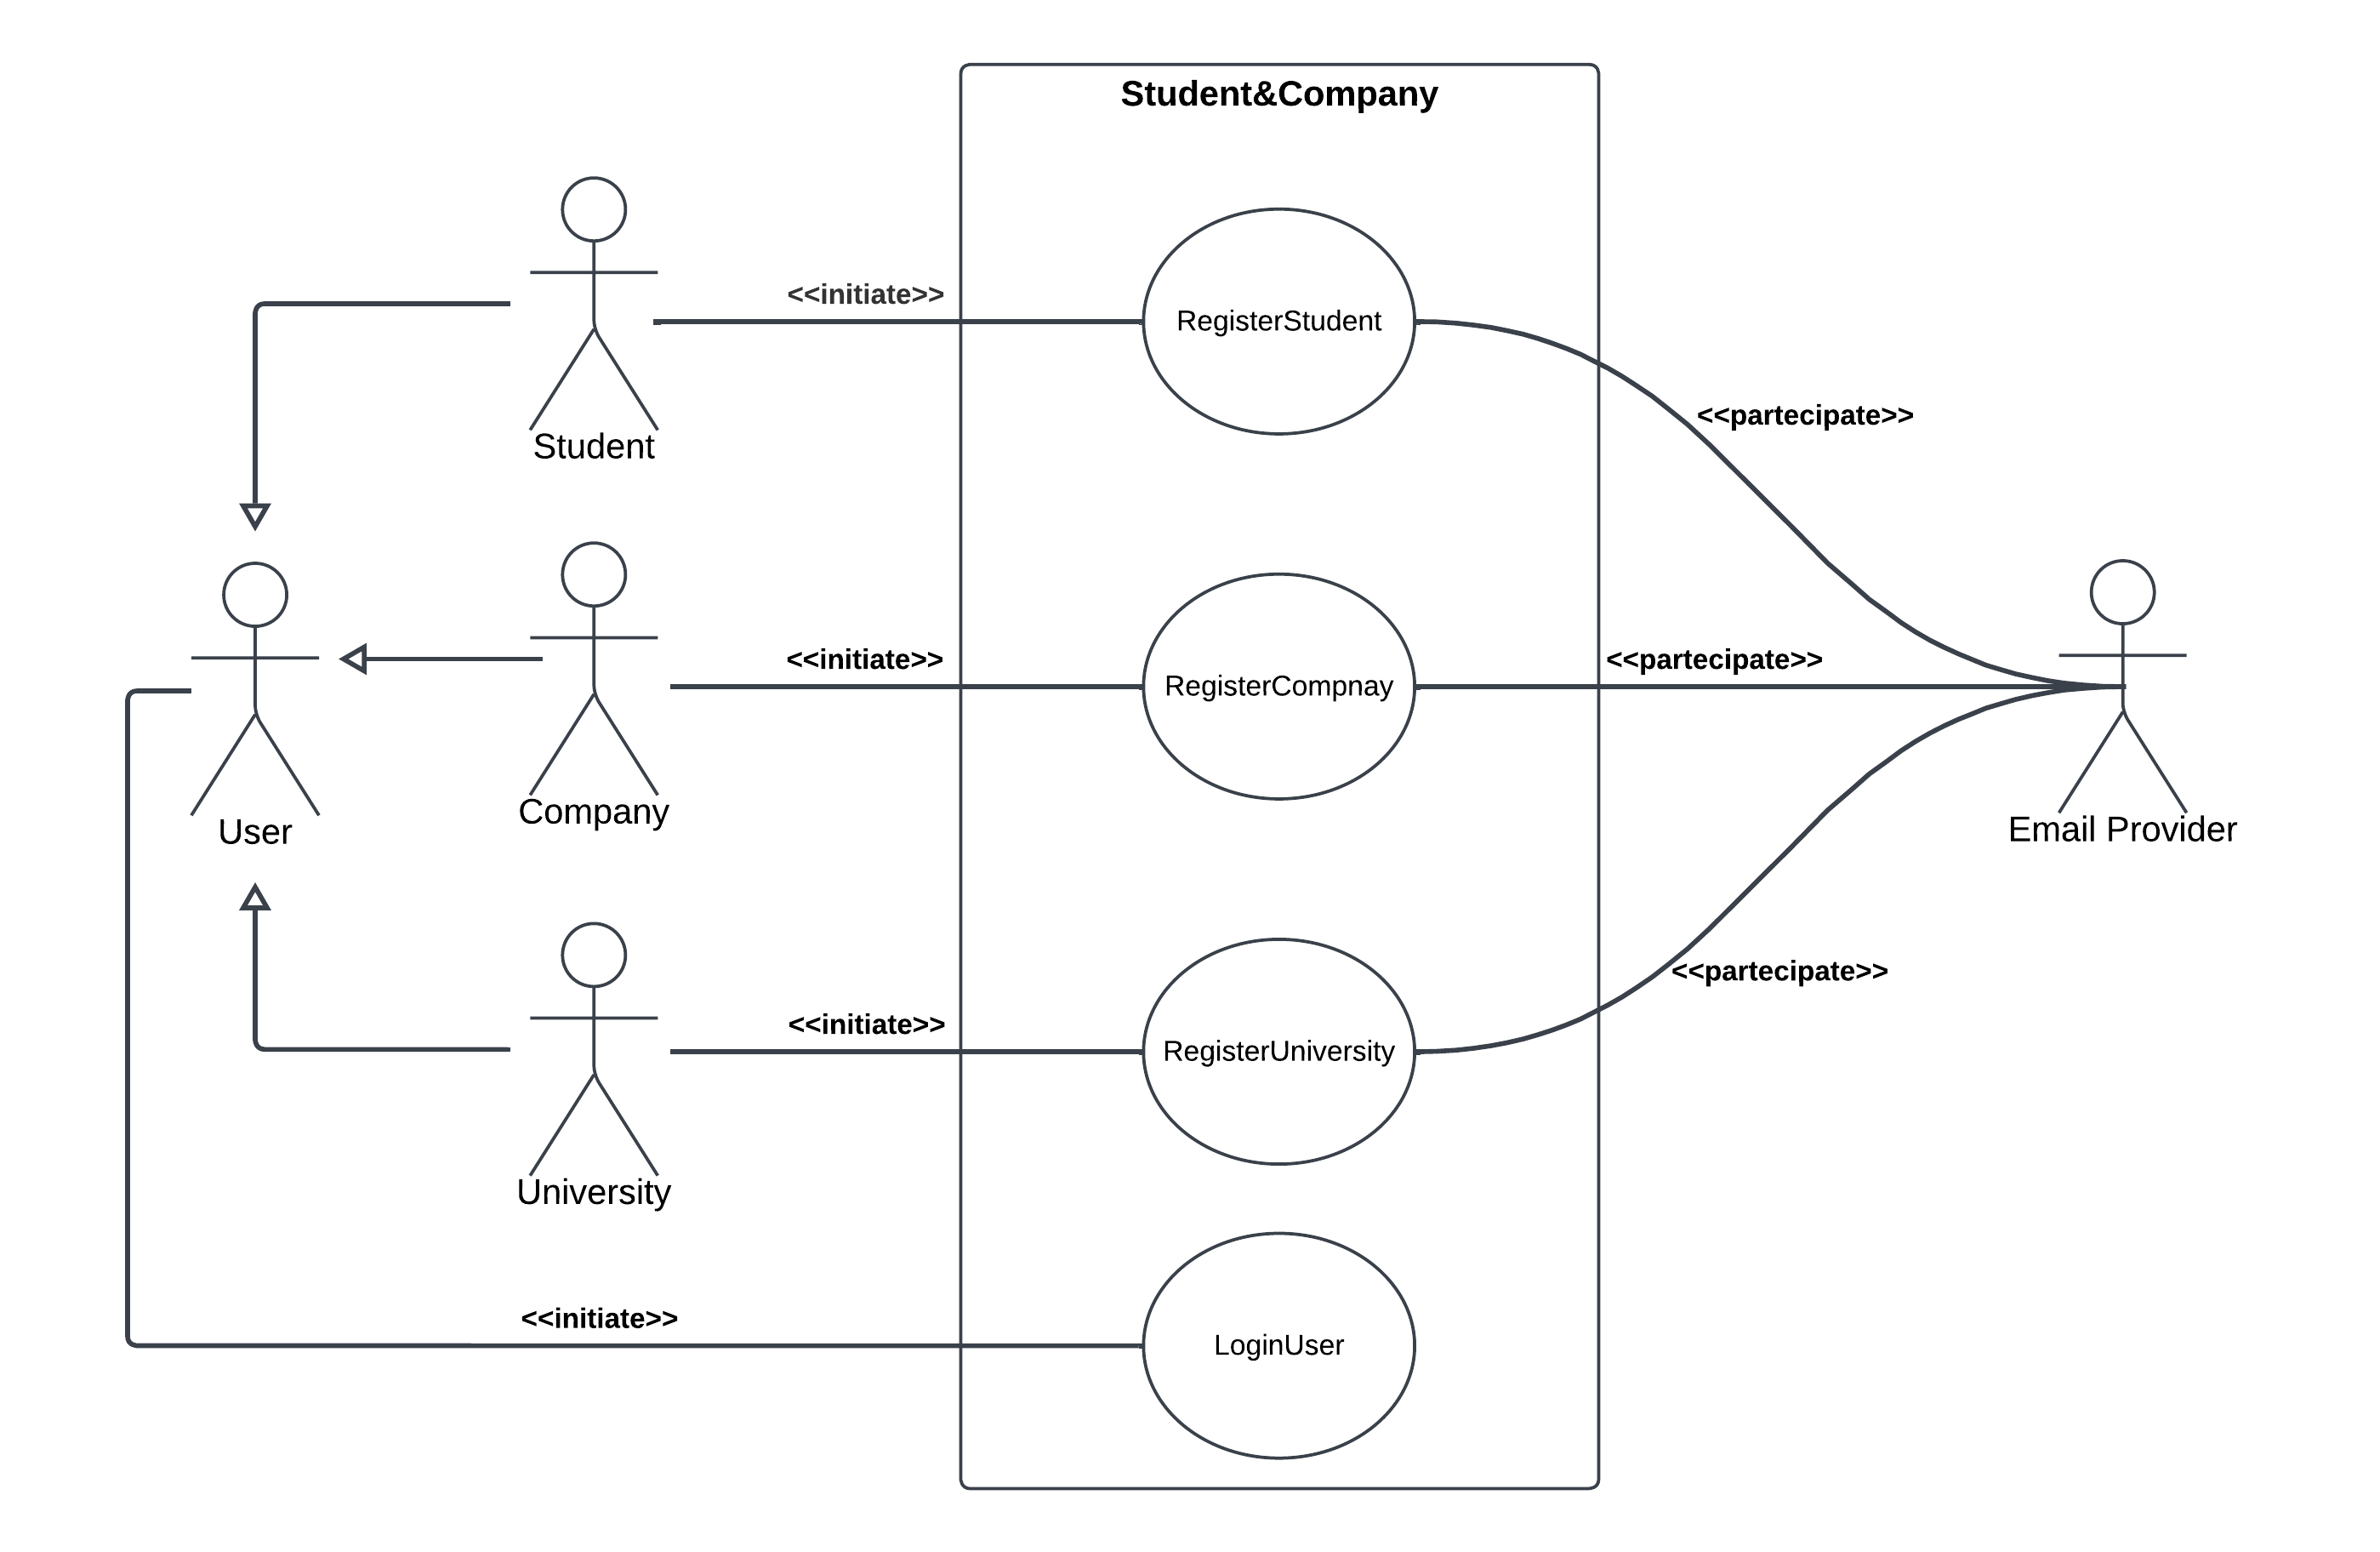
\includegraphics[width=1 \textwidth]{Diagrams/UseDiagrams/UserRegistrationUseCase.png}
    \caption{User Registration Use Case Diagram}
    \label{fig:UserRegistrationUseCaseDiagram}
\end{figure}
This diagram illustrates the User Registration and Login process, for all Users. It shows how the different use case for the registration, based on the User type, and how the login process is generic and common for all Users
\clearpage.
\begin{figure}[H]
    \centering
    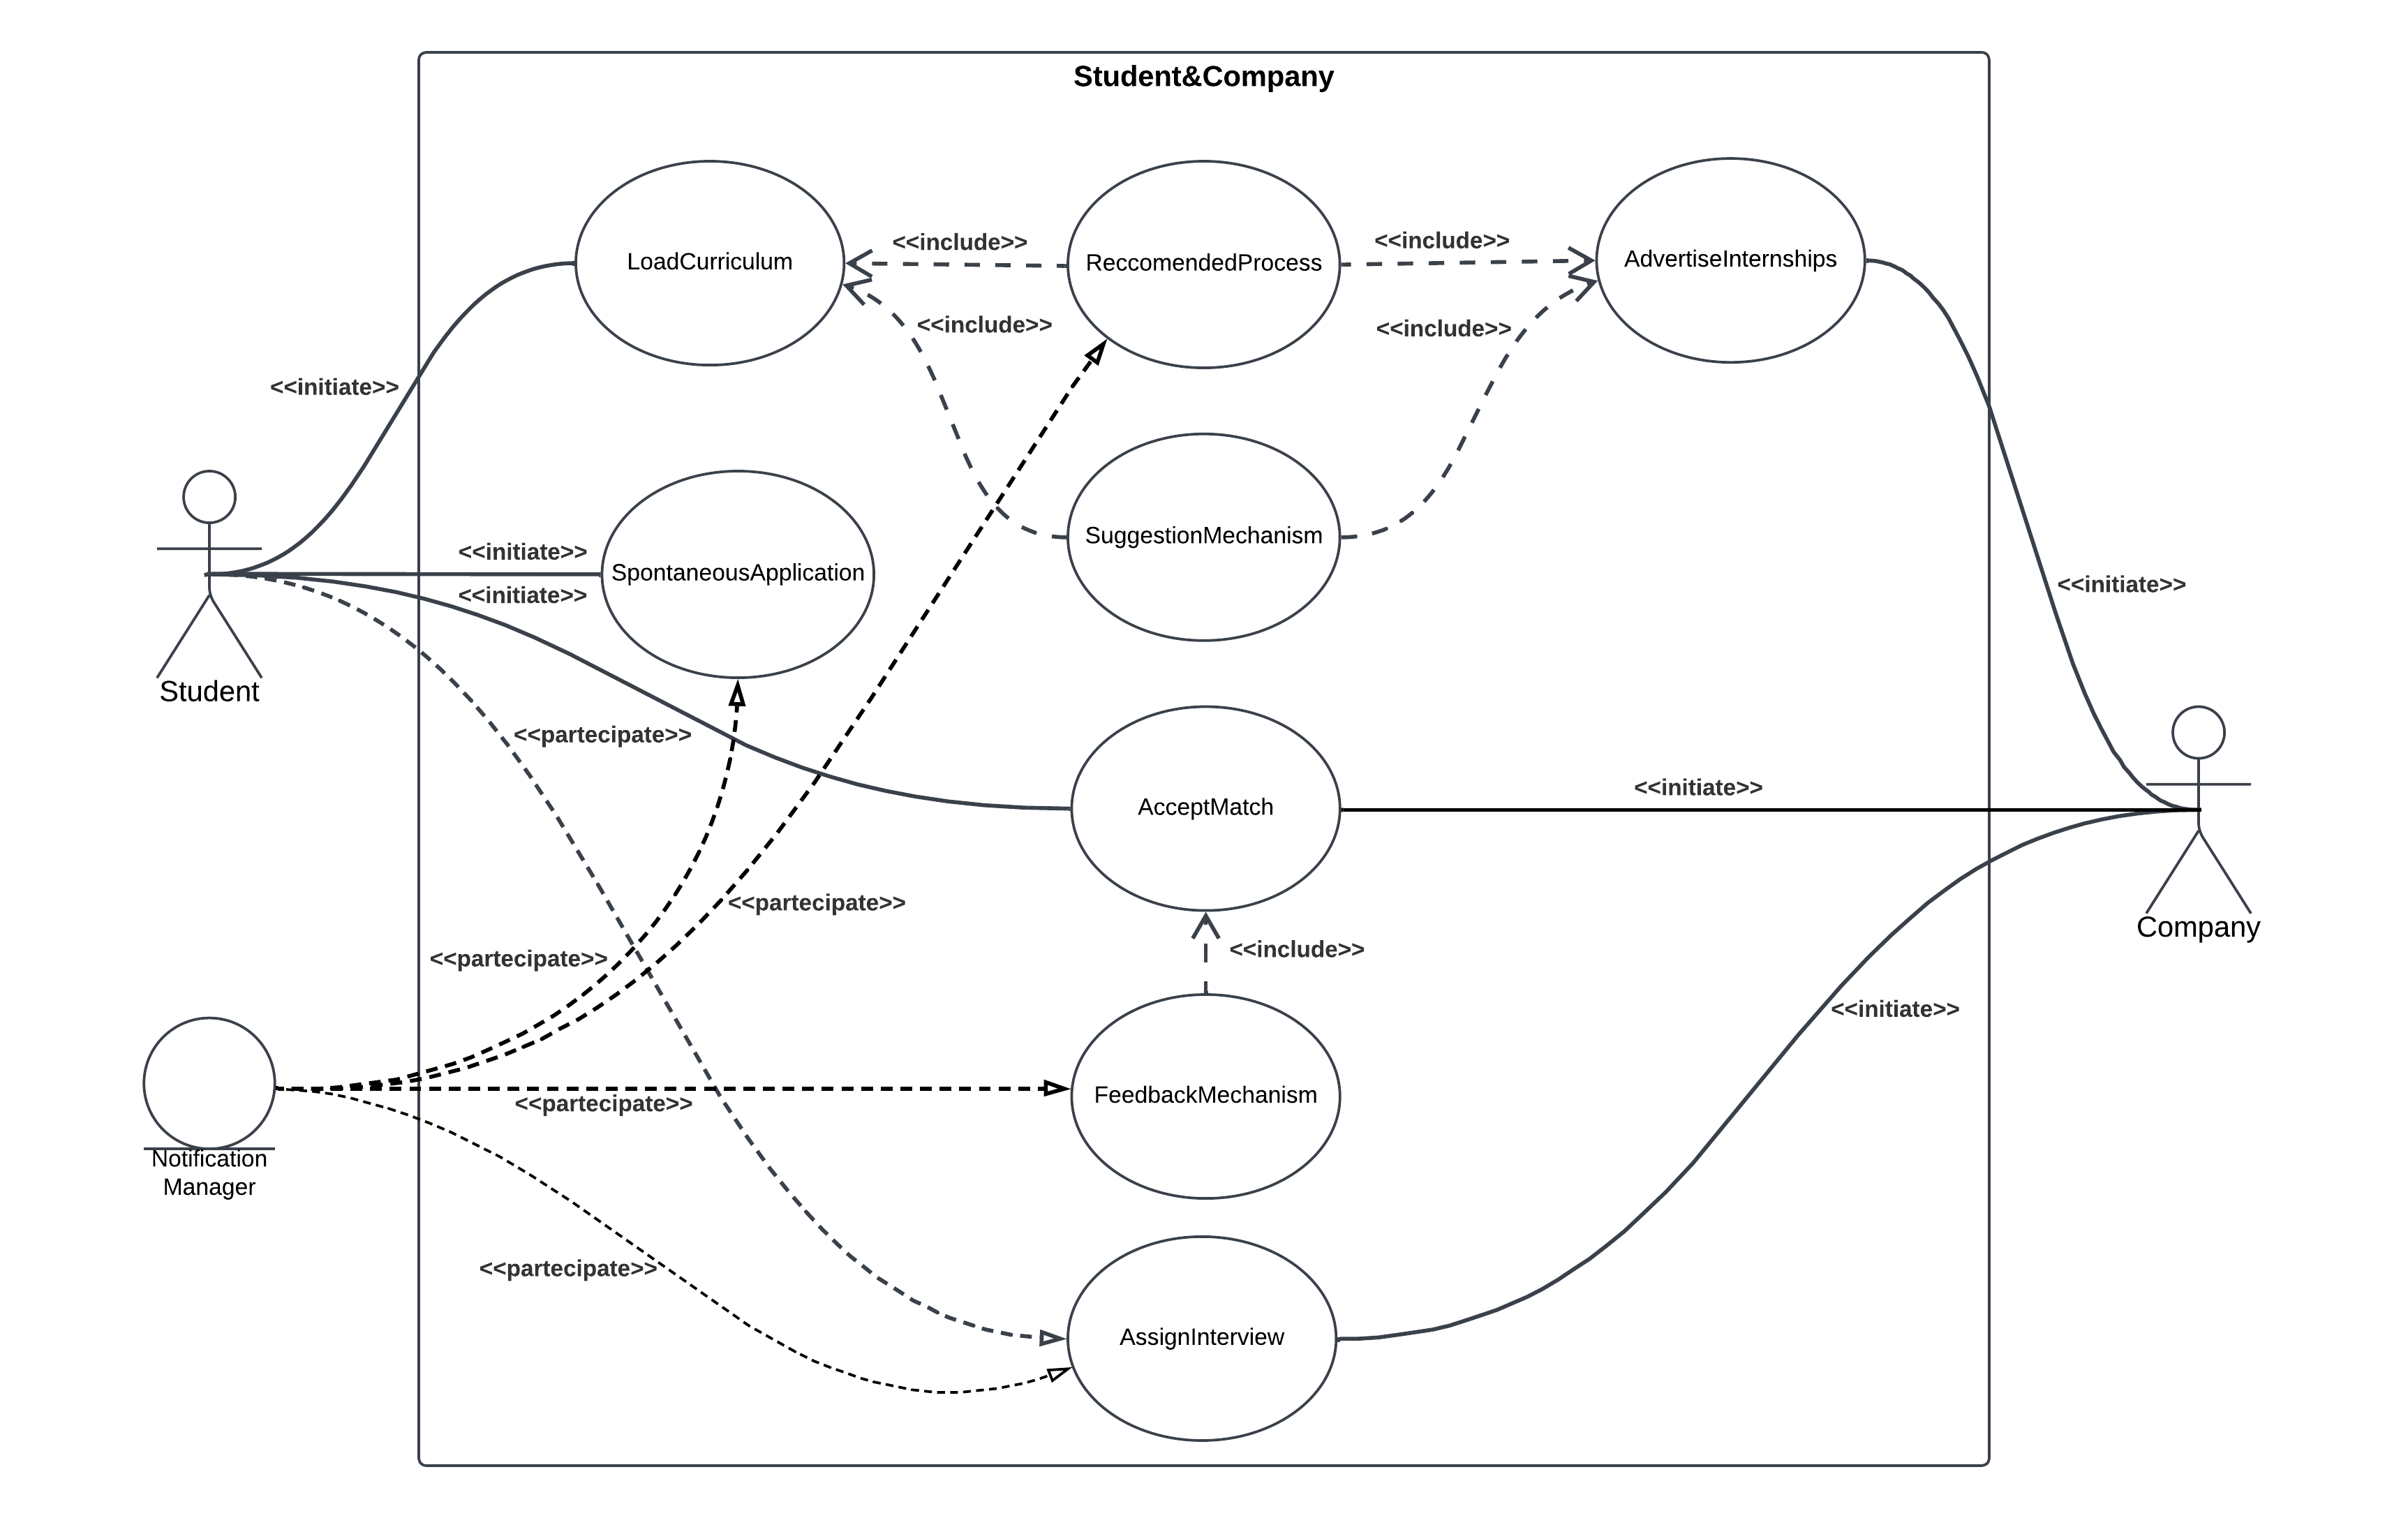
\includegraphics[width=1 \textwidth]{Diagrams/UseDiagrams/Student Company Use Case.png}
    \caption{Student and Company Use Case Diagram}
    \label{fig:StudentCompanyUseCaseDiagram}
\end{figure}
This diagram illustrates the main functionalities of the platform, such as the loading of CV or the creation of an Internship Offer. \\
This diagram both shows the different use cases that are specific to Students or Companies, and the common ones, such as the Acceptance of a Match. In such cases, the use case can be initiated by both actors.
\clearpage
\begin{figure}[H]
    \centering
    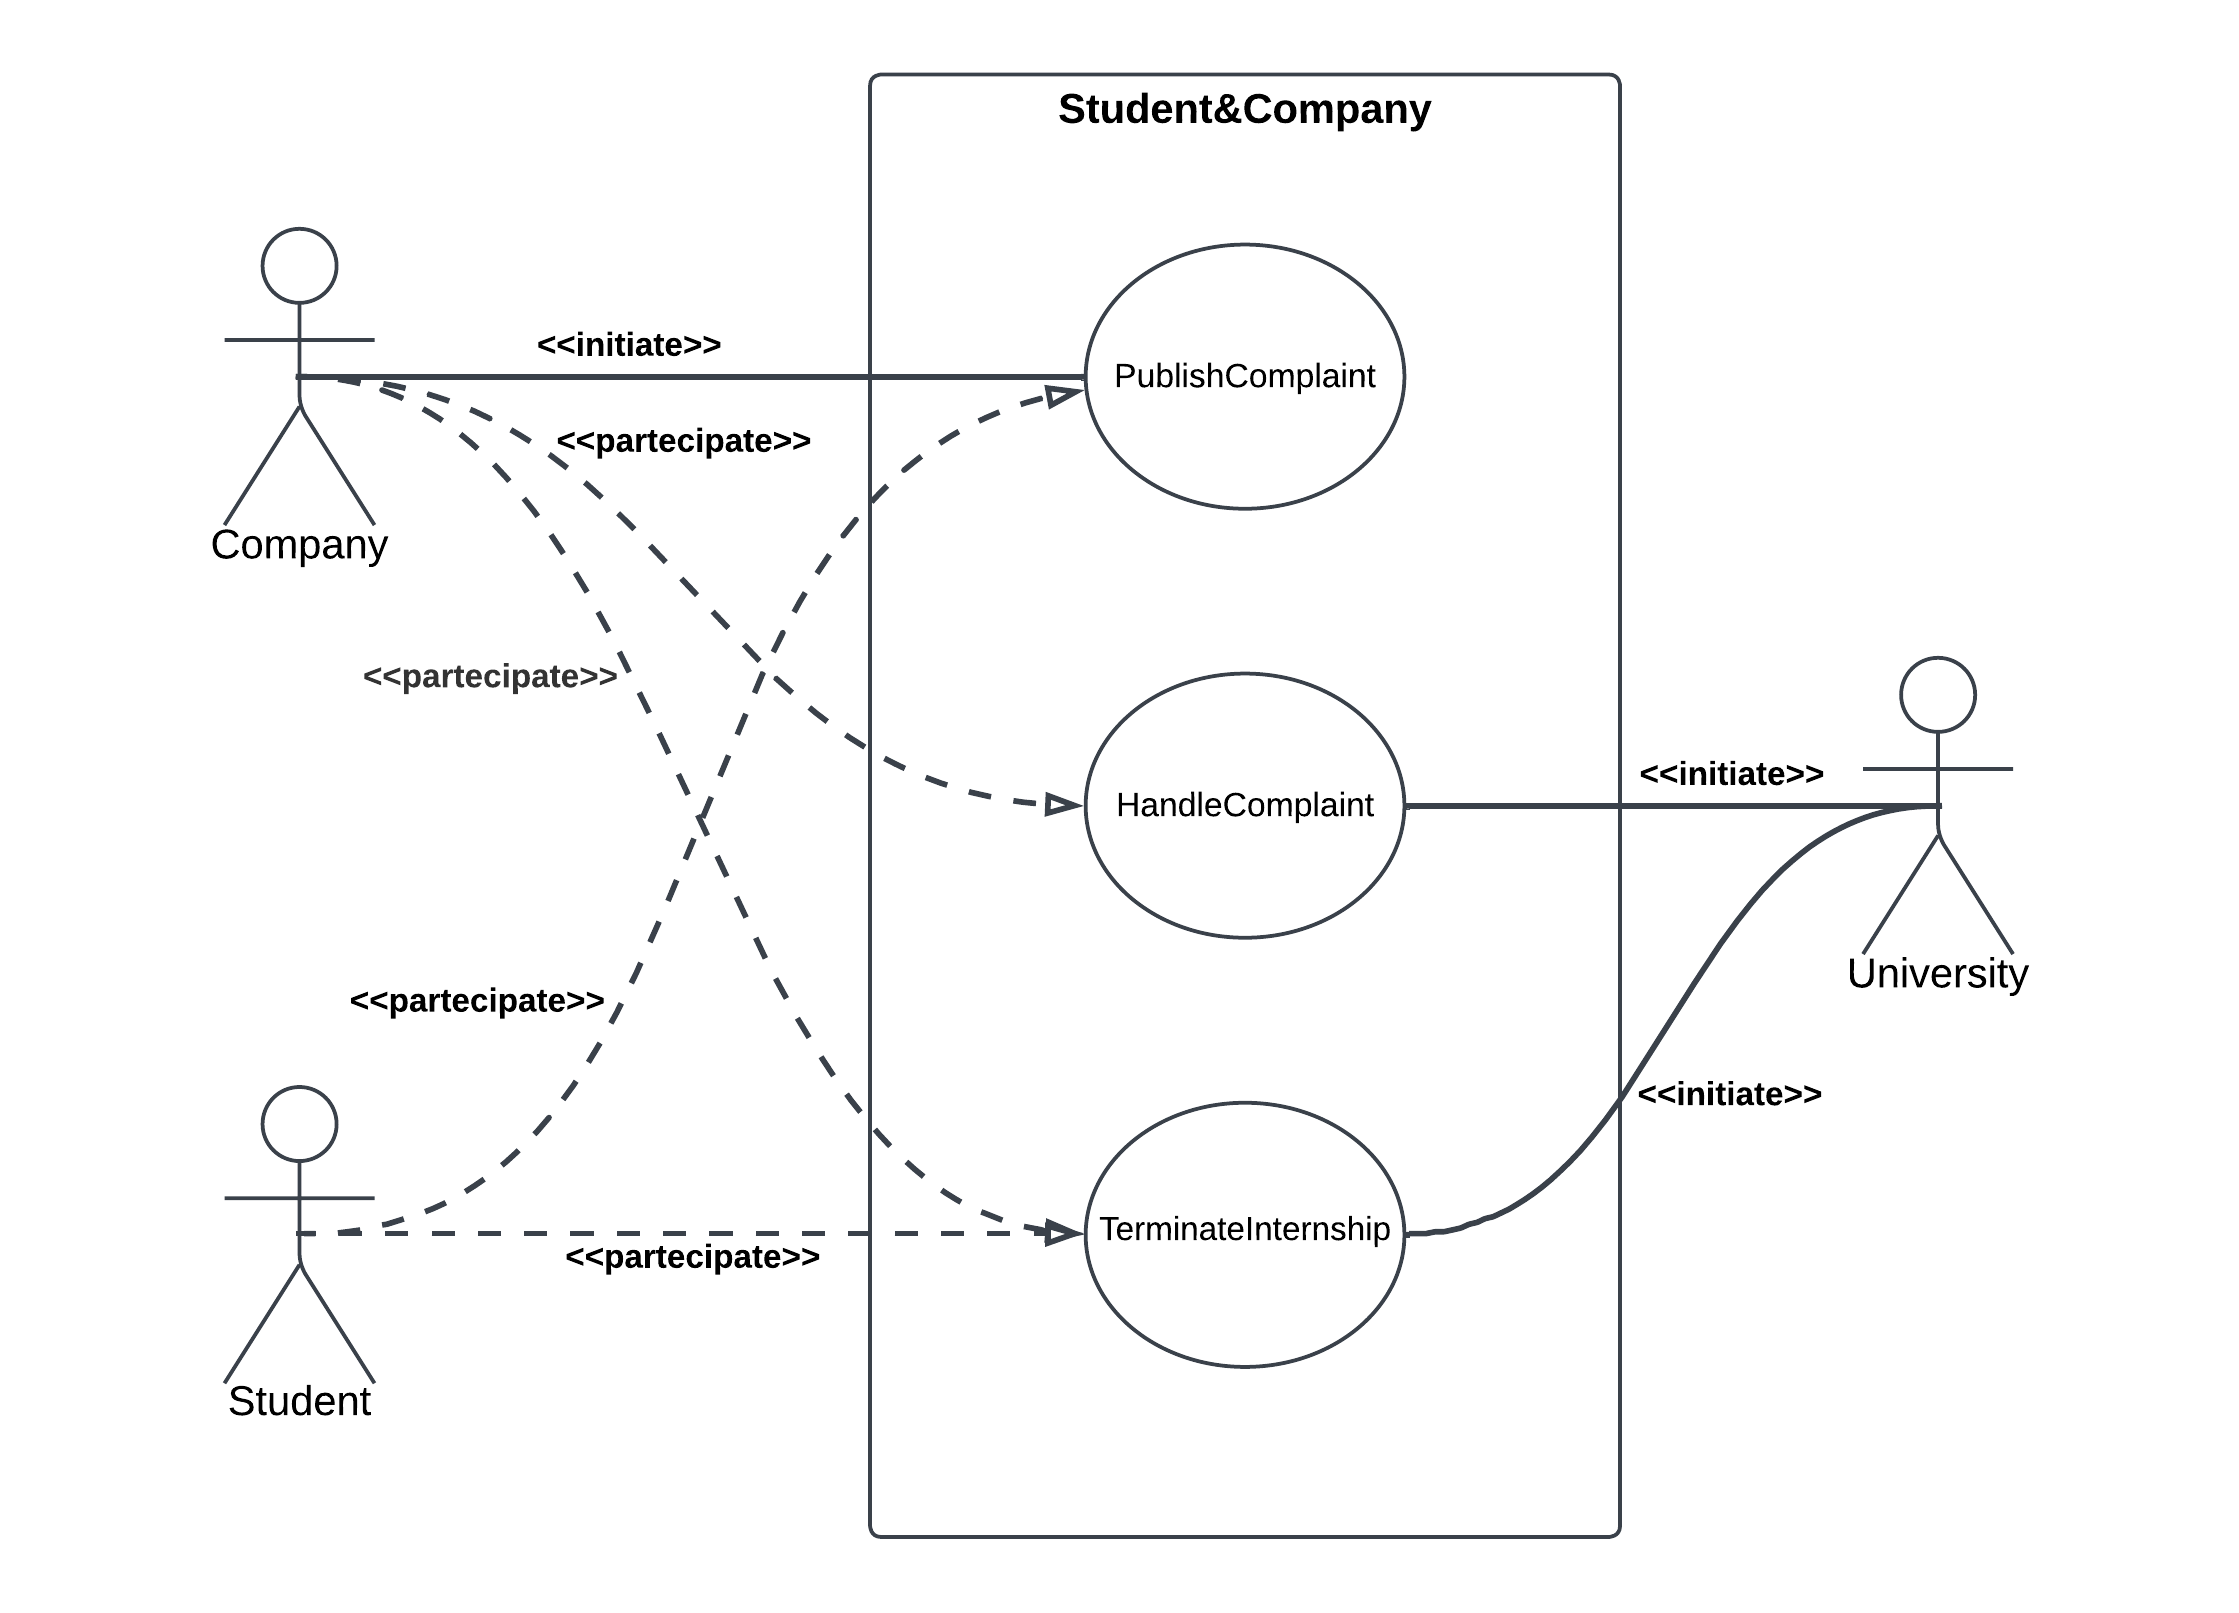
\includegraphics[width=1 \textwidth]{Diagrams/UseDiagrams/UniversityUseCaseDiagram.png}
    \caption{University and Complaint Use Case Diagram}
    \label{fig:UniveristyUseCaseDiagram}
\end{figure}
This diagram concentrates on the functionalities offered to Universities. It shows how a Participant can create a Complaint, and how the University can handle it. \\
More importantly, it shows that a complaint can be handled “as is” by the University, or it can be extended either by the other Participants that respond to such complaint or by the University itself that can interrupt an Ongoing Internship.
\clearpage

\subsubsection{Use Cases}

\begin{table}[H]
    \centering
    \begin{tabular}{|p{3cm}|p{12cm}|}
    \hline
    \multicolumn{2}{|c|}{\textbf{RegisterStudent}} \\ \hline
    Actor & 
    \begin{itemize}
        \item Student
        \item Email Provider
    \end{itemize} \\ \hline
    Entry Condition & The user is not logged in. \\ \hline
    Event Flow & 
    \begin{enumerate}         
        \item The Student presses the “Sign up” button situated on the dashboard.
        \item The platform opens the sign-up page.
        \item The Student selects the “Student” option, provides the required information (name, surname, date of birth, institutional email, optionally personal email, password, University name among those available) and click the “Sign Up” button.
        \item The platform validates the email and checks if it is unique.
        \item The platform registers the Student and sends a confirmation email to the provided email address through the Email Provider.
        \item The platform shows a message to the Student to confirm the registration.
        \item The Student confirms the registration by clicking on the link in the email.
        \item The platform confirms the registration and activates the account.
        \item The Student is redirected to the platform's dashboard.
    \end{enumerate} \\ \hline
    Exit Condition & The Student is registered and logged in. \\ \hline
    Exception & 
    \begin{itemize}
        \item The Student provides incorrect information.
        \item The Student does not confirm the registration.
        \item The email is already in use.
    \end{itemize} \\ \hline
    \end{tabular}
    \caption{[UC1]: Student registration use case}
    \label{tab:UC1}
\end{table}
\clearpage
\begin{table}[H]
    \centering
    \begin{tabular}{|p{3cm}|p{12cm}|}
    \hline
    \multicolumn{2}{|c|}{\textbf{RegisterCompany}} \\ \hline
    Actor & 
    \begin{itemize}
        \item Company
        \item Email Provider
    \end{itemize} \\ \hline
    Entry Condition & The user is not logged in \\ \hline
    Event Flow &
    \begin{enumerate}         
        \item The Company presses the “Sign up” button situated on the dashboard.
        \item The platform open the sign-up page.
        \item The Company selects the “Company” option, provides the required information (Company name, Company headquarters address, VAT number, email, and password) and click the “Sign Up” button.
        \item The platform checks if the VAT number and the email are unique
        \item The platform sends a confirmation email to the provided email address through the Email Provider.
        \item The platform shows a message to the Company to confirm the registration.
        \item The Company confirms the registration by clicking on the link in the email.
        \item The platform confirms the registration and activates the account.
        \item The Company is redirected to the platform's Dashboard.
    \end{enumerate} \\ \hline
    Exit Condition & The Company is registered and logged in. \\ \hline
    Exception & 
    \begin{itemize}
        \item The Company provides incorrect information.
        \item The Company does not confirm the registration.
        \item The VAT number or the email is already in use.
    \end{itemize} \\ \hline
    \end{tabular}
    \caption{[UC2]: Company registration use case}
    \label{tab:UC2}
\end{table}

\begin{table}[H]
    \centering
    \begin{tabular}{|p{3cm}|p{12cm}|}
    \hline
    \multicolumn{2}{|c|}{\textbf{RegisterUniversity}} \\ \hline
    Actor & 
    \begin{itemize}
        \item University
        \item Email Provider
    \end{itemize} \\ \hline
    Entry Condition & The user is not logged in. \\ \hline
    Event Flow &
    \begin{enumerate}         
        \item The University presses the “Sign up” button situated on the dashboard.
        \item The platform open the sign-up page.
        \item The University selects the “University” option, provides the required information (University Name, University description, VAT number, email of the University office that will manage the internship program, and password) and click the “Sign Up” button.
        \item The platform checks if the VAT number and the email are unique
        \item The platform sends a confirmation email to the provided email address through the Email Provider.
        \item The platform shows a message to the University to confirm the registration.
        \item The University confirms the registration by clicking on the link in the email.
        \item The platform confirms the registration and activates the account.
        \item The University is redirected to the platform's Dashboard.
    \end{enumerate} \\ \hline
    Exit Condition & The University is registered and logged in.\\ \hline
    Exceptions &
    \begin{itemize}
        \item The University provides incorrect information.
        \item The University does not confirm the registration.
        \item The VAT number or the email is already in use.
    \end{itemize} \\ \hline
    \end{tabular}
    \caption{[UC3]: University registration use case}
    \label{tab:UC3}
\end{table}

\begin{table}[H]
    \centering
    \begin{tabular}{|p{3cm}|p{12cm}|}
    \hline
    \multicolumn{2}{|c|}{\textbf{LoginUser}} \\ \hline
    Actor & 
    \begin{itemize}
        \item User
    \end{itemize}\\ \hline
    Entry Condition & The user is not logged in \\ \hline
    Event Flow &
    \begin{enumerate}         
        \item The User presses the “Sign in” button situated on the dashboard.
        \item The platform open the sign-in page.
        \item The user provides their email and password.
        \item The platform validates the credentials.
        \item The platform confirms the credentials and logs in the User.
        \item The User is redirected to the platform's Dashboard.
    \end{enumerate} \\ \hline
    Exit Condition & The User is logged in. \\ \hline
    Exceptions &
    \begin{itemize}
        \item The User provides incorrect email or password.
    \end{itemize} \\ \hline
    \end{tabular}
    \caption{[UC4]: User login use case}
    \label{tab:UC4}
\end{table}

\begin{table}[H]
    \centering
    \begin{tabular}{|p{3cm}|p{12cm}|}
    \hline
    \multicolumn{2}{|c|}{\textbf{LoadCurriculum}} \\ \hline
    Actor & 
    \begin{itemize}
        \item Student
        \item Notification Manager
        \item Company
    \end{itemize}\\ \hline
    Entry Condition & The Student is logged in \\ \hline
    Event Flow &
    \begin{enumerate}         
        \item The Student presses the “CV” menu button situated on the dashboard.
        \item The platform opens the Curriculum page.
        \item The Student fills the form with the required information (current level of education, known languages, technical skills, a photo of himself, a brief description of his interests and hobbies etc...) and click the “Submit CV” button.
        \item The platform publishes the CV.
        \item The platform generates a list of matching internships based on the CV.
        \item The platform provides feedback and suggestions to improve the CV.
        \item The Student is redirected to his account page.
        \item The platform notifies the new matching Companies through the Notification Manager. 
    \end{enumerate} \\ \hline
    Exit Condition & The Student's CV is uploaded. \\ \hline
    Exception & 
    \begin{itemize} 
        \item The Student provides invalid or partial information.
    \end{itemize} \\ \hline
    \end{tabular}
    \caption{[UC5]: Student uploads Curriculum use case}
    \label{tab:UC5}
\end{table}

\begin{table}[H]
    \centering
    \begin{tabular}{|p{3cm}|p{12cm}|}
    \hline
    \multicolumn{2}{|c|}{\textbf{AdvertiseInternships}} \\ \hline
    Actor & 
    \begin{itemize}
        \item Company
        \item Notification Manager
        \item Student
    \end{itemize}\\ \hline
    Entry Condition & The Company is logged in\\ \hline
    Event Flow &
    \begin{enumerate}         
        \item The Company presses the “Internship Offers” button situated on the dashboard.
        \item The Platform opens the Internships page.
        \item The Company presses the “Create Internship” button.
        \item The platform shows the Internship creation form.
        \item The Company fills the form with the required information (Internship title, description, start date and duration, office address, required skills and benefits offered) and click the “Submit Internship” button.
        \item The platform publishes the Internship.
        \item The platform generates a list of matching Students based on the Internship.
        \item The system provides feedback and suggestions to improve the internship description.
        \item The Company is redirected to the Internships page.
        \item The platform notifies the new matching Students through the Notification Manager. 
    \end{enumerate} \\ \hline
    Exit Condition & The Internship is created and published.\\ \hline
    Exception & 
    \begin{itemize}        
        \item The Company provides invalid or partial information.
    \end{itemize} \\ \hline
    \end{tabular}
    \caption{[UC6]: Company advertises an Internship use case}
    \label{tab:UC6}
\end{table}

\begin{table}[H]
    \centering
    \begin{tabular}{|p{3cm}|p{12cm}|}
    \hline
    \multicolumn{2}{|c|}{\textbf{SpontaneousApplication}} \\ \hline
    Actor & 
    \begin{itemize}
        \item Student
        \item Company
        \item Notification Manager
    \end{itemize}\\ \hline
    Entry Condition & The Student is logged in and has his CV uploaded. \\ \hline
    Event Flow &
    \begin{enumerate}         
        \item The Student presses the “Browse Internships” button situated on the dashboard.
        \item The platform opens the global Internships page.
        \item The Student presses the “Apply” button on one of the available Internships.
        \item The platform adds the application to the Company and Student list of applications.
        \item The platform notifies the Company of the Spontaneous Application through the Notification Manager.
    \end{enumerate} \\ \hline
    Exit Condition & The application is successfully submitted to the Company.\\ \hline
    Exception & 
    \begin{itemize}       
        \item Internship is no longer available.
    \end{itemize} \\ \hline
    \end{tabular}
    \caption{[UC7]: Student submits Spontaneous Application use case}
    \label{tab:UC7}
\end{table}

\begin{table}[H]
    \centering
    \begin{tabular}{|p{3cm}|p{12cm}|}
    \hline
    \multicolumn{2}{|c|}{\textbf{AcceptMatch}} \\ \hline
    Actor & 
    \begin{itemize}
        \item Participant
        \item Notification Manager
    \end{itemize}\\ \hline
    Entry Condition & A Match is generated between the Student and the Company's Internship and the Student has his CV uploaded. \\ \hline
    Event Flow &  
    \begin{enumerate}
        \item The Participant presses the “Recommendations Process” button situated on the dashboard.
        \item The platform opens the respective Recommendations pages.
        \item The Participant accepts the Match.
        \item The platform stores the result.
        \item If the other party has already accepted the Match, the platform adds the Interview to the Student and the Company's list of Interviews and notifies both parties through the Notification Manager.
    \end{enumerate} \\ \hline
    Exit Condition & The Match is successfully accepted by the participant.\\ \hline
    Exception & 
    \begin{itemize}
        \item None
    \end{itemize} \\ \hline
    \end{tabular}
    \caption{[UC8]: Company or Student accepts Match use case}
    \label{tab:UC8}
\end{table}

\begin{table}[H]
    \centering
    \begin{tabular}{|p{3cm}|p{12cm}|}
    \hline
    \multicolumn{2}{|c|}{\textbf{FeedbackMechanism}} \\ \hline
    Actor & 
    \begin{itemize}
        \item Participant
    \end{itemize}\\ \hline
    Entry Condition & The Participant is logged in. \\ \hline
    Event Flow &      
    \begin{enumerate}         
        \item The Participant presses the “Recommendations Process” button situated on the dashboard.
        \item The platform opens the respective Recommendations pages.
        \item The Participant accept or decline the Match.
        \item The platform asks for feedback about the Match.
        \item The Participant submits the feedback.
        \item The platform stores the feedback.
    \end{enumerate} \\ \hline
    Exit Condition & Feedback is successfully provided. \\ \hline
    Exception & 
    \begin{itemize}     
        \item None
    \end{itemize} \\ \hline
    \end{tabular}
    \caption{[UC9]: Feedback is asked upon Match result use case}
    \label{tab:UC9}
\end{table}

\begin{table}[H]
    \centering
    \begin{tabular}{|p{3cm}|p{12cm}|}
    \hline
    \multicolumn{2}{|c|}{\textbf{SuggestionMechanism}} \\ \hline
    Actor & 
    \begin{itemize}
        \item Participant
    \end{itemize}\\ \hline
    Entry Condition & A Student has uploaded his CV or a Company has created an Internship.\\ \hline
    Event Flow & 
    \begin{enumerate}         
        \item The platform analyses the Student's CV or the Company's Internship.
        \item The platform generates a list of suggestions to improve the CV or the Internship description.
        \item The platform displays a notification on the Participant's dashboard page.
        \item The Participant open the notification.
        \item The platform displays the suggestions.
    \end{enumerate} \\ \hline
    Exit Condition & Suggestions are successfully provided. \\ \hline
    Exception & 
    \begin{itemize}        
        \item No valuable suggestions are found.  
    \end{itemize} \\ \hline
    \end{tabular}
    \caption{[UC10]: Suggestion mechanism use case}
    \label{tab:UC10}
\end{table}

\begin{table}[H]
    \centering
    \begin{tabular}{|p{3cm}|p{12cm}|}
    \hline
    \multicolumn{2}{|c|}{\textbf{AssignInterview}} \\ \hline
    Actor & 
    \begin{itemize}
        \item Company
        \item Student
        \item Notification Manager
    \end{itemize} \\ \hline
    Entry Condition & A Match is accepted by both parties or the Company has accepted a Spontaneous Application. \\ \hline
    Event Flow &      
    \begin{enumerate}         
        \item The Company presses the “Interviews” button situated on the dashboard.
        \item The platform opens the Interviews page.
        \item The Company selects an Interview in the “ToBeSubmitted” state.
        \item The platform shows the Interview creation form.
        \item The Company fills the form with the required information (open and closed questions, deadline and additional infos) and click the “Submit Interview” button.
        \item The platform sends the form to the Student, updates his Interview status and notifies him thorough the Notification Manager.
        \item The Company is redirected to the Interviews page.
    \end{enumerate} \\ \hline
    Exit Condition & The Interview is created and submitted to the Student. \\ \hline
    Exception & 
    \begin{itemize}         
        \item None
    \end{itemize} \\ \hline
    \end{tabular}
    \caption{[UC11]: Company assigns Interview to Student use case}
    \label{tab:UC11}
\end{table}

\begin{table}[H]
    \centering
    \begin{tabular}{|p{3cm}|p{12cm}|}
    \hline
    \multicolumn{2}{|c|}{\textbf{PublishComplaint}} \\ \hline
    Actor & 
    \begin{itemize}
        \item Company
        \item Student
        \item University
        \item Notification Manager
    \end{itemize} \\ \hline
    Entry Condition & There is an Ongoing Internship between the relative Company and Student.\\ \hline
    Event Flow &      
    \begin{enumerate}         
        \item The Company presses the “Communications” button situated on the dashboard.
        \item The platform opens the Communications page.
        \item The Company presses the “Create Complaint” button.
        \item The platform shows the Complaint creation form.
        \item The Company fills the form with the required information (Student's name, Internship title, description of the problem) and click the “Submit Complaint” button.
        \item The platform publishes the Complaint.
        \item The platform notifies the Student and the University through the Notification Manager.
    \end{enumerate} \\ \hline
    Exit Condition & The Complaint is created and published. \\ \hline
    Exception & 
    \begin{itemize}       
        \item None
    \end{itemize} \\ \hline
    \end{tabular}
    \caption{[UC12]: Company publishes Complaint use case}
    \label{tab:UC12}
\end{table}

\begin{table}[H]
    \centering
    \begin{tabular}{|p{3cm}|p{12cm}|}
    \hline
    \multicolumn{2}{|c|}{\textbf{RespondToComplaint}} \\ \hline
    Actor & 
    \begin{itemize}
        \item User
        \item Notification Manager
    \end{itemize} \\ \hline
    Entry Condition & The User has an active Complaint.\\ \hline
    Event Flow &      
    \begin{enumerate}         
        \item The Student or the Company presses the “Communications” button situated on the dashboard.
        \item The platform opens the Communications page.
        \item The User presses the target complaint.
        \item The platform shows the relative Complaint page.
        \item The User responds to the Complaint and submits the message.
        \item The platform notifies the other Users involved in the Complaint about the response through the Notification Manager.
    \end{enumerate} \\ \hline
    Exit Condition & The response is successfully published, and involved Users are notified.\\ \hline
    Exception & 
    \begin{itemize}       
        \item None
    \end{itemize} \\ \hline
    \end{tabular}
    \caption{[UC13]: User responds to a Complaint use case}
    \label{tab:UC13}
\end{table}


\begin{table}[H]
    \centering
    \begin{tabular}{|p{3cm}|p{12cm}|}
    \hline
    \multicolumn{2}{|c|}{\textbf{HandleComplaint}} \\ \hline
    Actor & 
    \begin{itemize}
        \item University
        \item Student
        \item Company
    \end{itemize}\\ \hline
    Entry Condition & There is an active Complaint regarding the Company and a Student of the University.\\ \hline
    Event Flow &      
    \begin{enumerate}         
        \item The University presses the “Communications” button situated on the dashboard.
        \item The platform opens the Communications page.
        \item The University presses the target complaint.
        \item The platform shows the relative Complaint page.
        \item The University presses the “Close Complaint” button, writes a final message and submits.
        \item The platform will close the relative Complaint.
        \item The platform notifies the Student and the Company about the resolution of the Complaint through the Notification Manager.
    \end{enumerate} \\ \hline
    Exit Condition & The Complaint is closed.\\ \hline
    Exception & 
    \begin{itemize}         
        \item None
    \end{itemize} \\ \hline    
    \end{tabular}
    \caption{[UC14]: University handles Complaint use case}
    \label{tab:UC14}
\end{table}

\begin{table}[H]
    \centering
    \begin{tabular}{|p{3cm}|p{12cm}|}
    \hline
    \multicolumn{2}{|c|}{\textbf{TerminateInternship}} \\ \hline
    Actor & 
    \begin{itemize}
        \item Student
        \item Company
        \item University
        \item Notification Manager
    \end{itemize}\\ \hline
    Entry Condition & There is an active Complaint regarding the Company and a Student of the University. \\ \hline
    Event Flow & 
    \begin{enumerate}         
        \item The University presses the “Communications” button situated on the dashboard.
        \item The platform opens the Communications page.
        \item The University presses the target complaint.
        \item The platform shows the relative Complaint page.
        \item The University presses the “Interrupt Internship” button.
        \item The platform will notify the Student and the Company about the interruption of the Internship through the Notification Manager and close the relative Complaint.
    \end{enumerate} \\ \hline
    Exit Condition & The Internship is interrupted, and the Complaint is closed. \\ \hline
    Exception & 
    \begin{itemize}         
        \item None
    \end{itemize} \\ \hline  
    \end{tabular}
    \caption{[UC15]: University terminates Internship use case}
    \label{tab:UC15}
\end{table}

\subsubsection{Sequence Diagrams}
The functions used in the sequence diagrams follow these conventional meanings:
\begin{itemize}
    \item \textbf{press(Button)}: Represents the action of a user pressing Button.
    \item \textbf{submit(Content)}: Indicates a user uploading Content to the platform.
    \item \textbf{showPage(Page)}: Displays the content of a specific Page.
    \item \textbf{showError(Error)}: Displays an error message indicating an issue that occurred.
    \item \textbf{showMessage(Message)}: Displays a generic message to the user.
    \item \textbf{notify(What, Who)}: Represents a notification forwarded to the NotificationManager regarding What and intended for Who.
    \item \textbf{check()}: Verifies the validity of the information provided by the user.
    \item \textbf{update(Data)}: Refers to internal processes that update database records with Data.
\end{itemize}
For readability, in all diagrams except the first four, the user login process is omitted. It is assumed that the user is already logged in and navigating the dashboard. Accordingly, the S\&C processes are depicted as already in progress.\\

\begin{figure}[H]
    \centering
    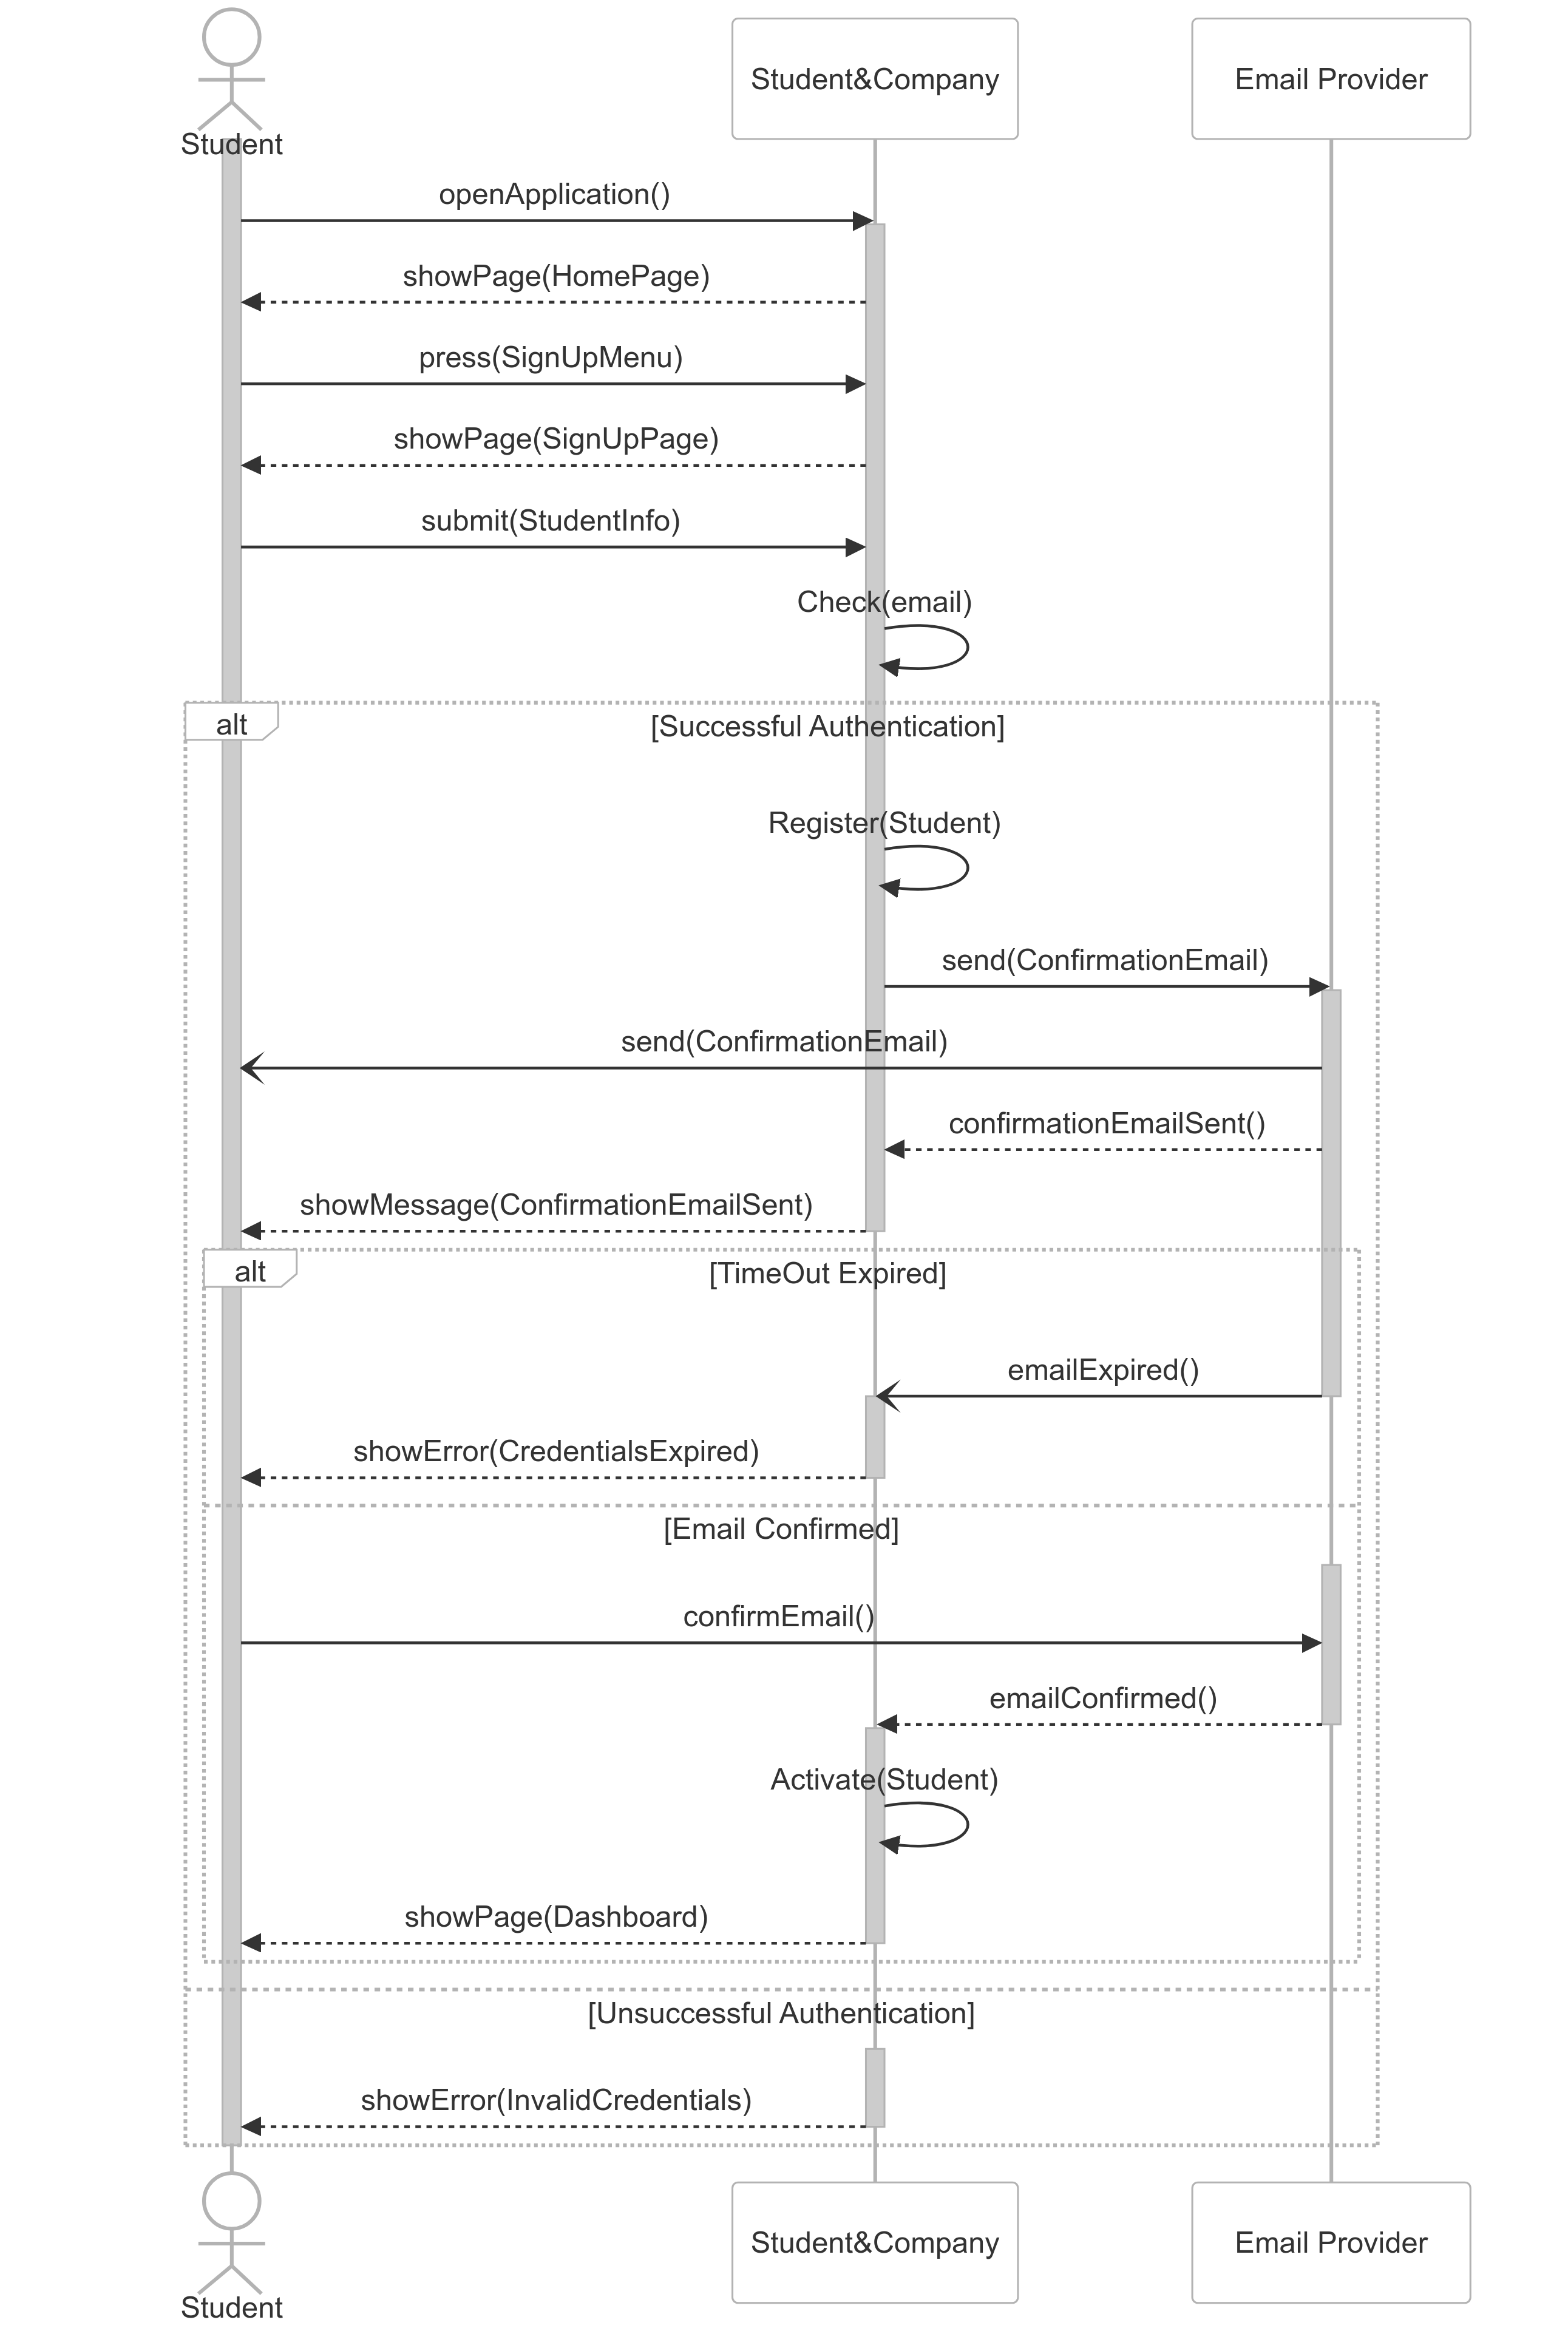
\includegraphics[width=0.75\textwidth]{Latex/Images/StudentSignUpSequenceDiagram.png}
    \caption{[SD1]: Student sign-up Sequence Diagram}
    \label{fig:SD1}
\end{figure}
\clearpage

\begin{figure}
    \centering
    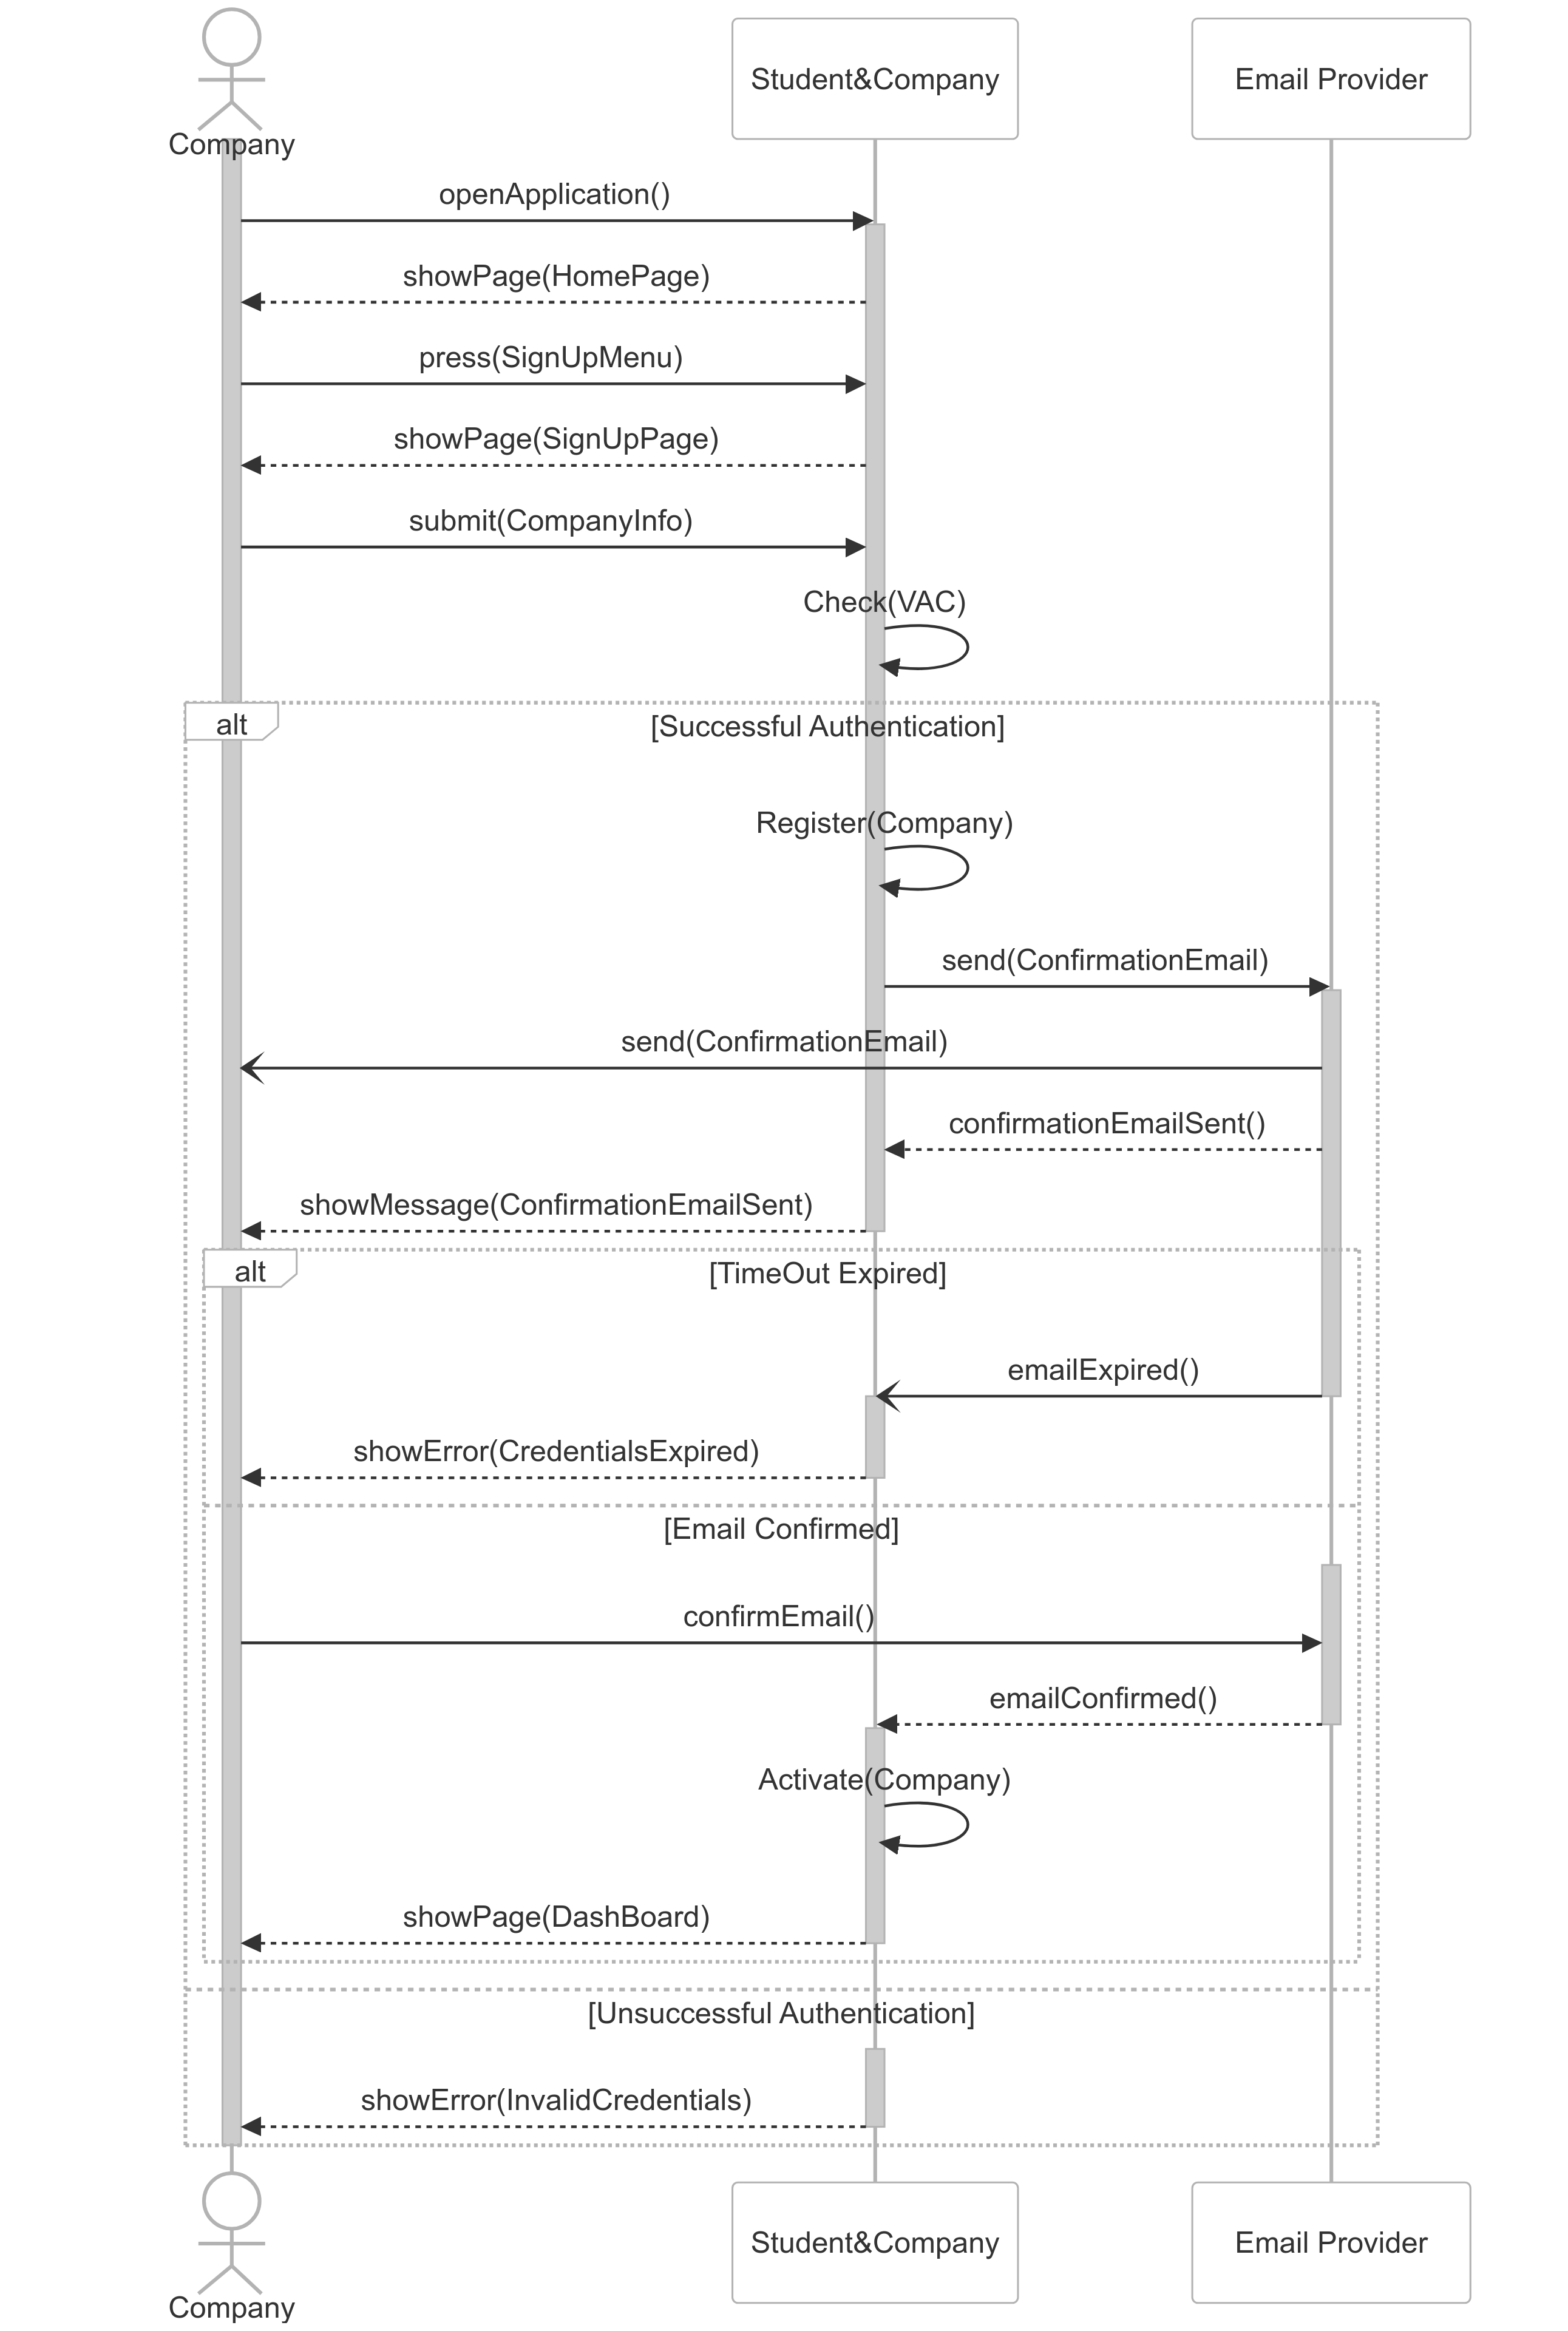
\includegraphics[width=0.8\textwidth]{Latex/Images/CompanySignUpSequenceDiagram.png}
    \caption{[SD2]: Company sign-up Sequence Diagram}
    \label{fig:SD2}
\end{figure}
\clearpage

\begin{figure}
    \centering
    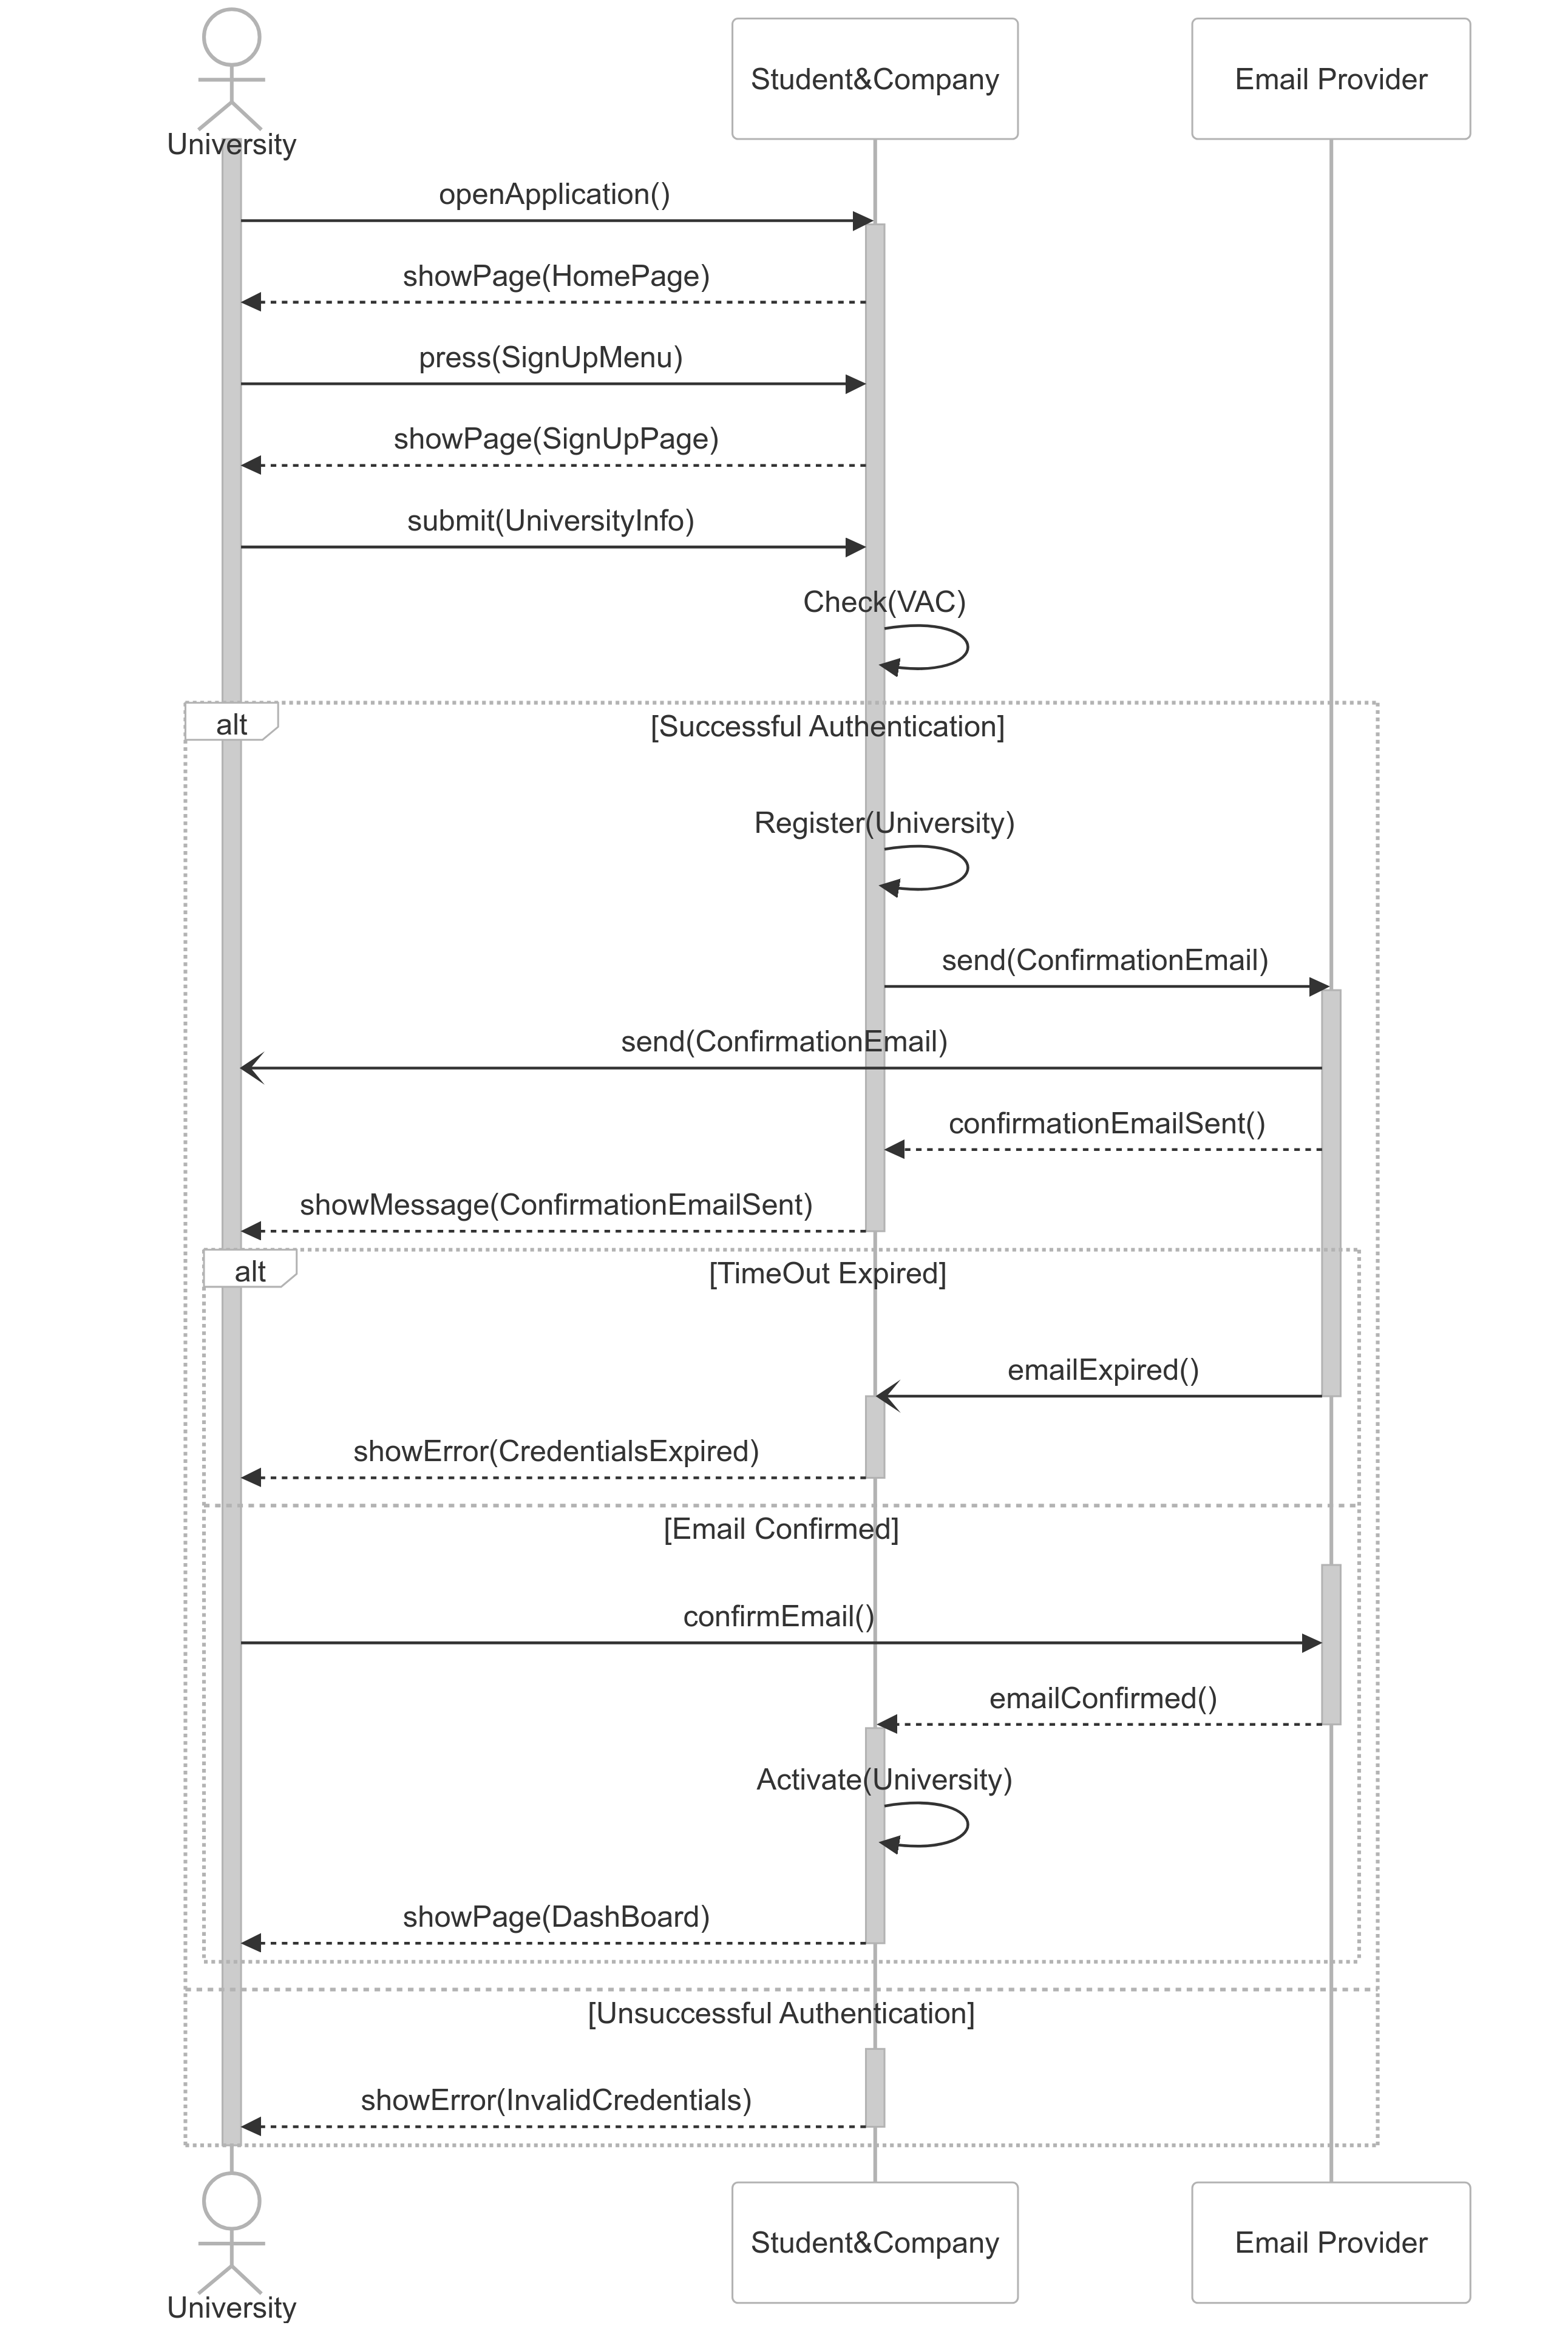
\includegraphics[width=0.8\textwidth]{Latex/Images/UniversitySignUpSequenceDiagram.png}
    \caption{[SD3]: University sign-up Sequence Diagram}
    \label{fig:SD3}
\end{figure}
\clearpage

\begin{figure}
    \centering
    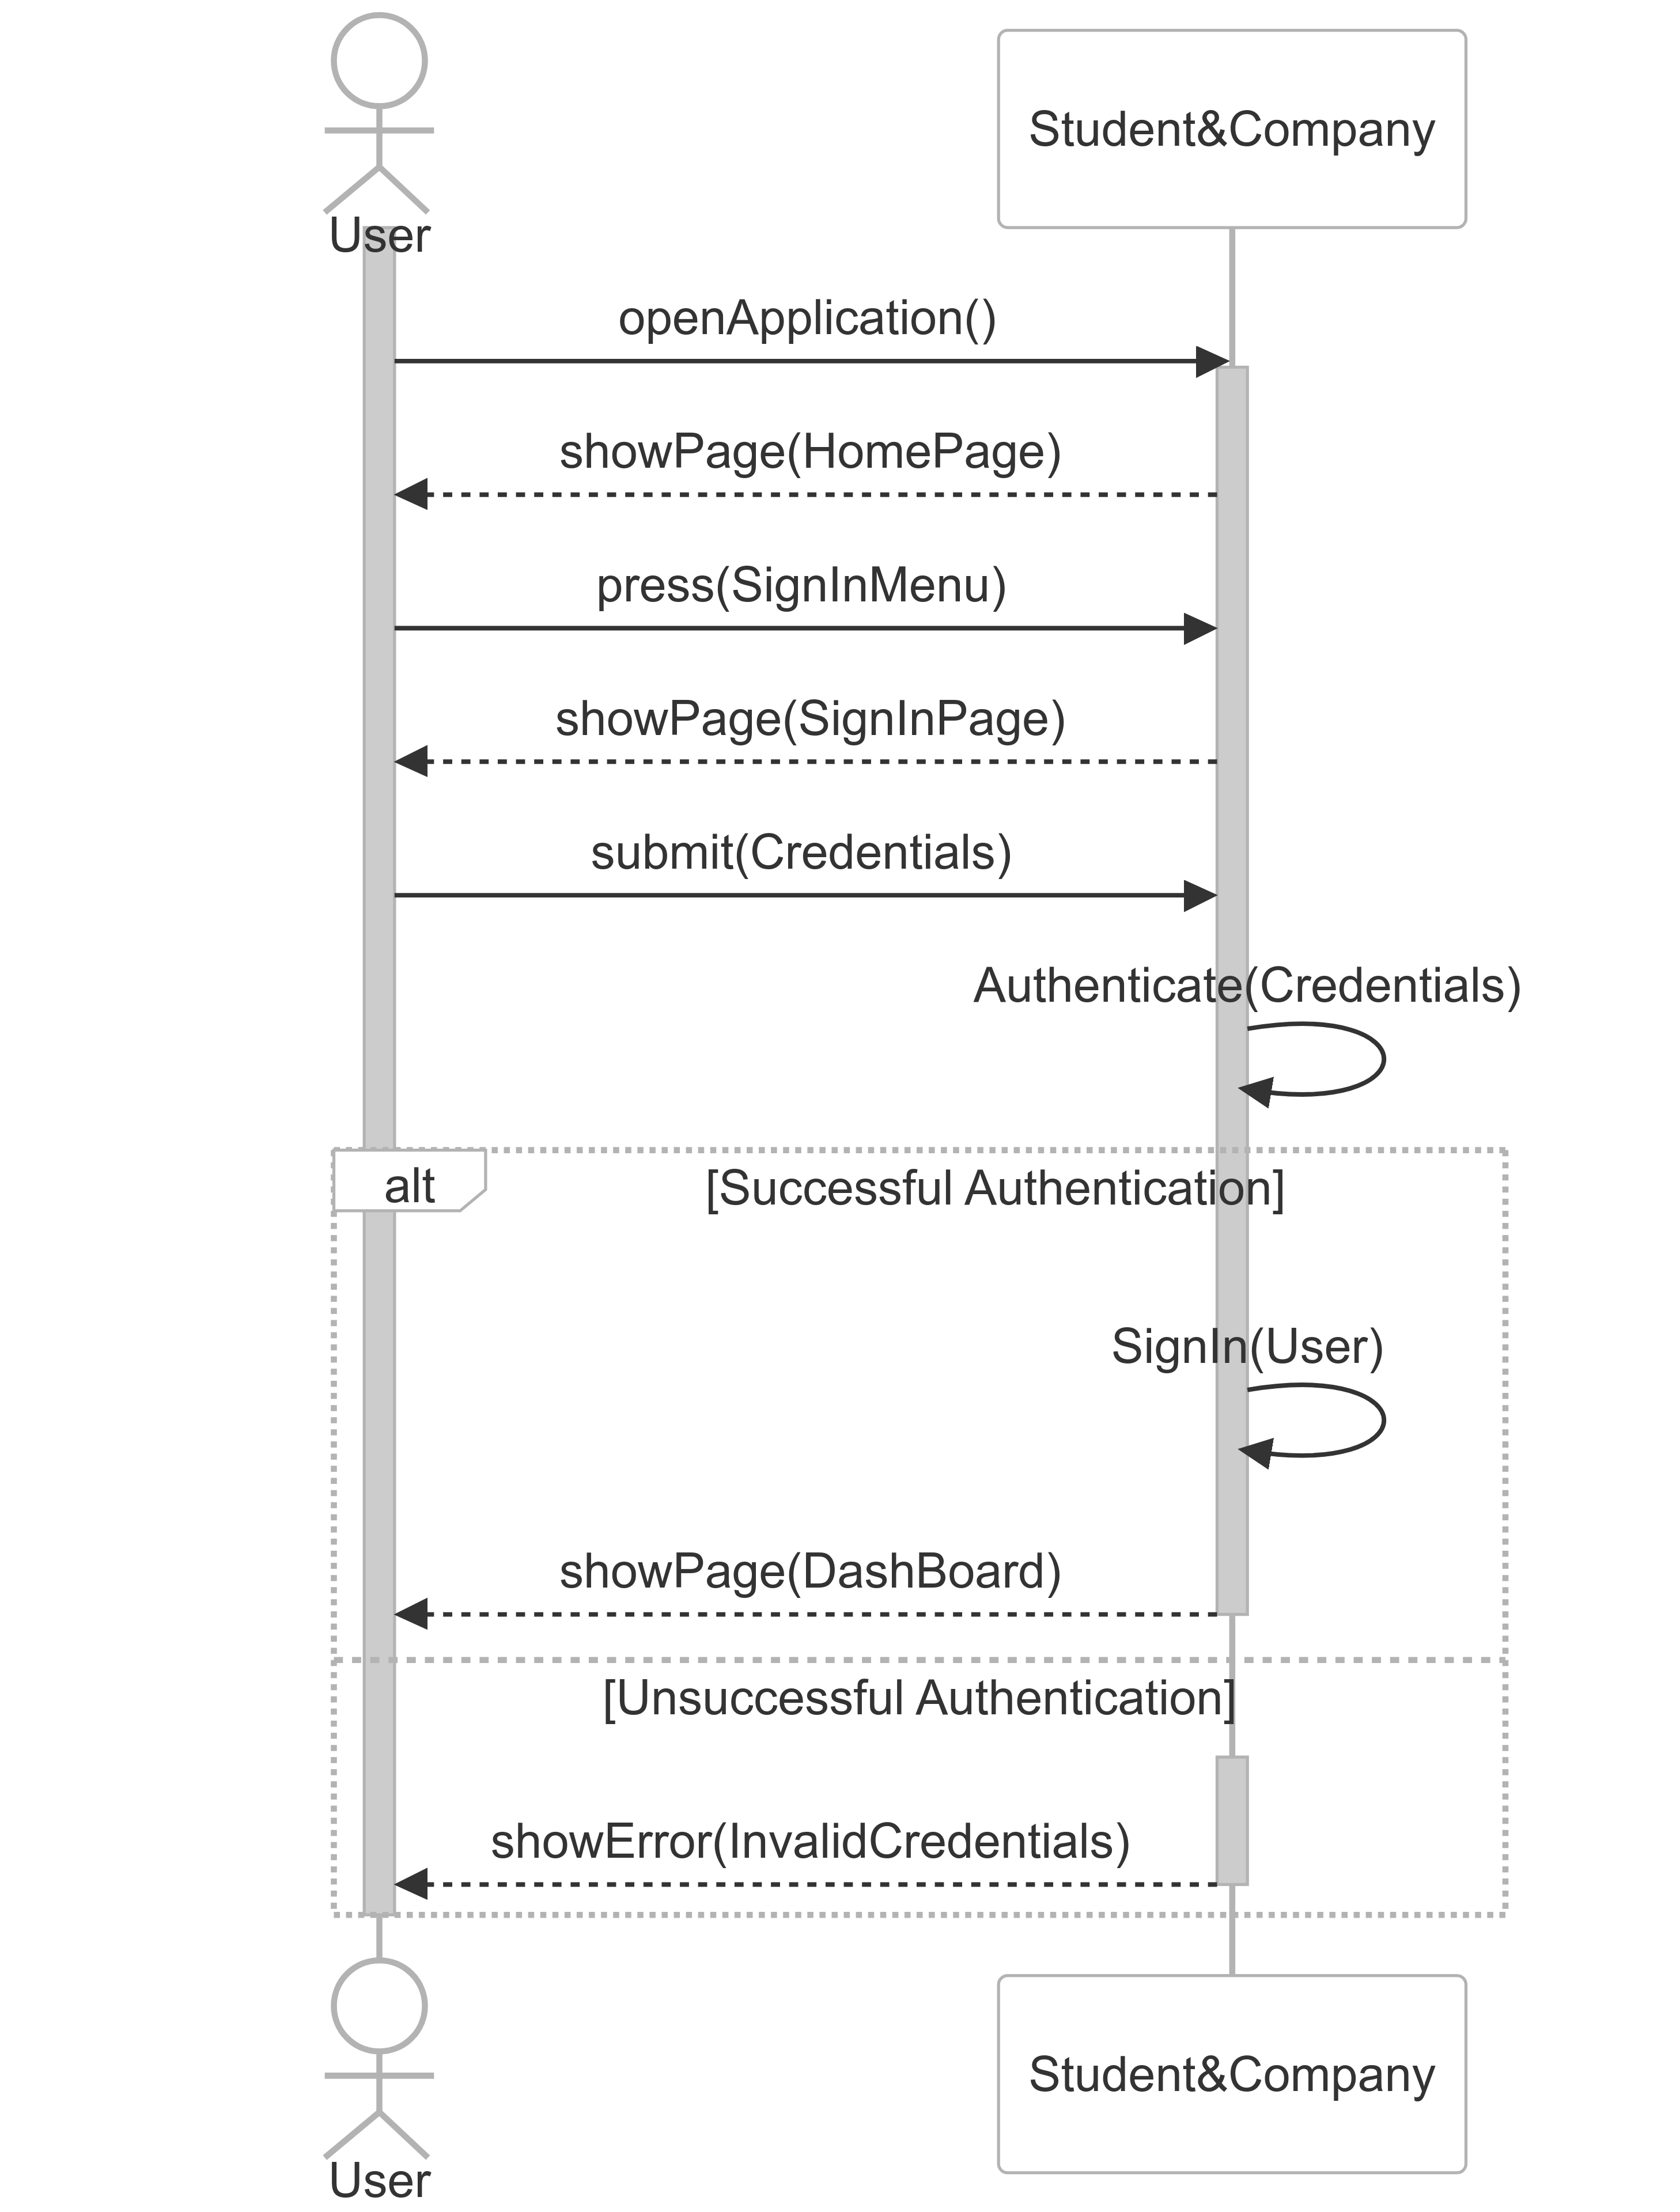
\includegraphics[width=0.6\textwidth]{Latex/Images/UserSignInSequenceDiagram.png}
    \caption{[SD4]: User sign-in Sequence Diagram}
    \label{fig:SD4}
\end{figure}
\clearpage

\begin{figure}
    \centering
    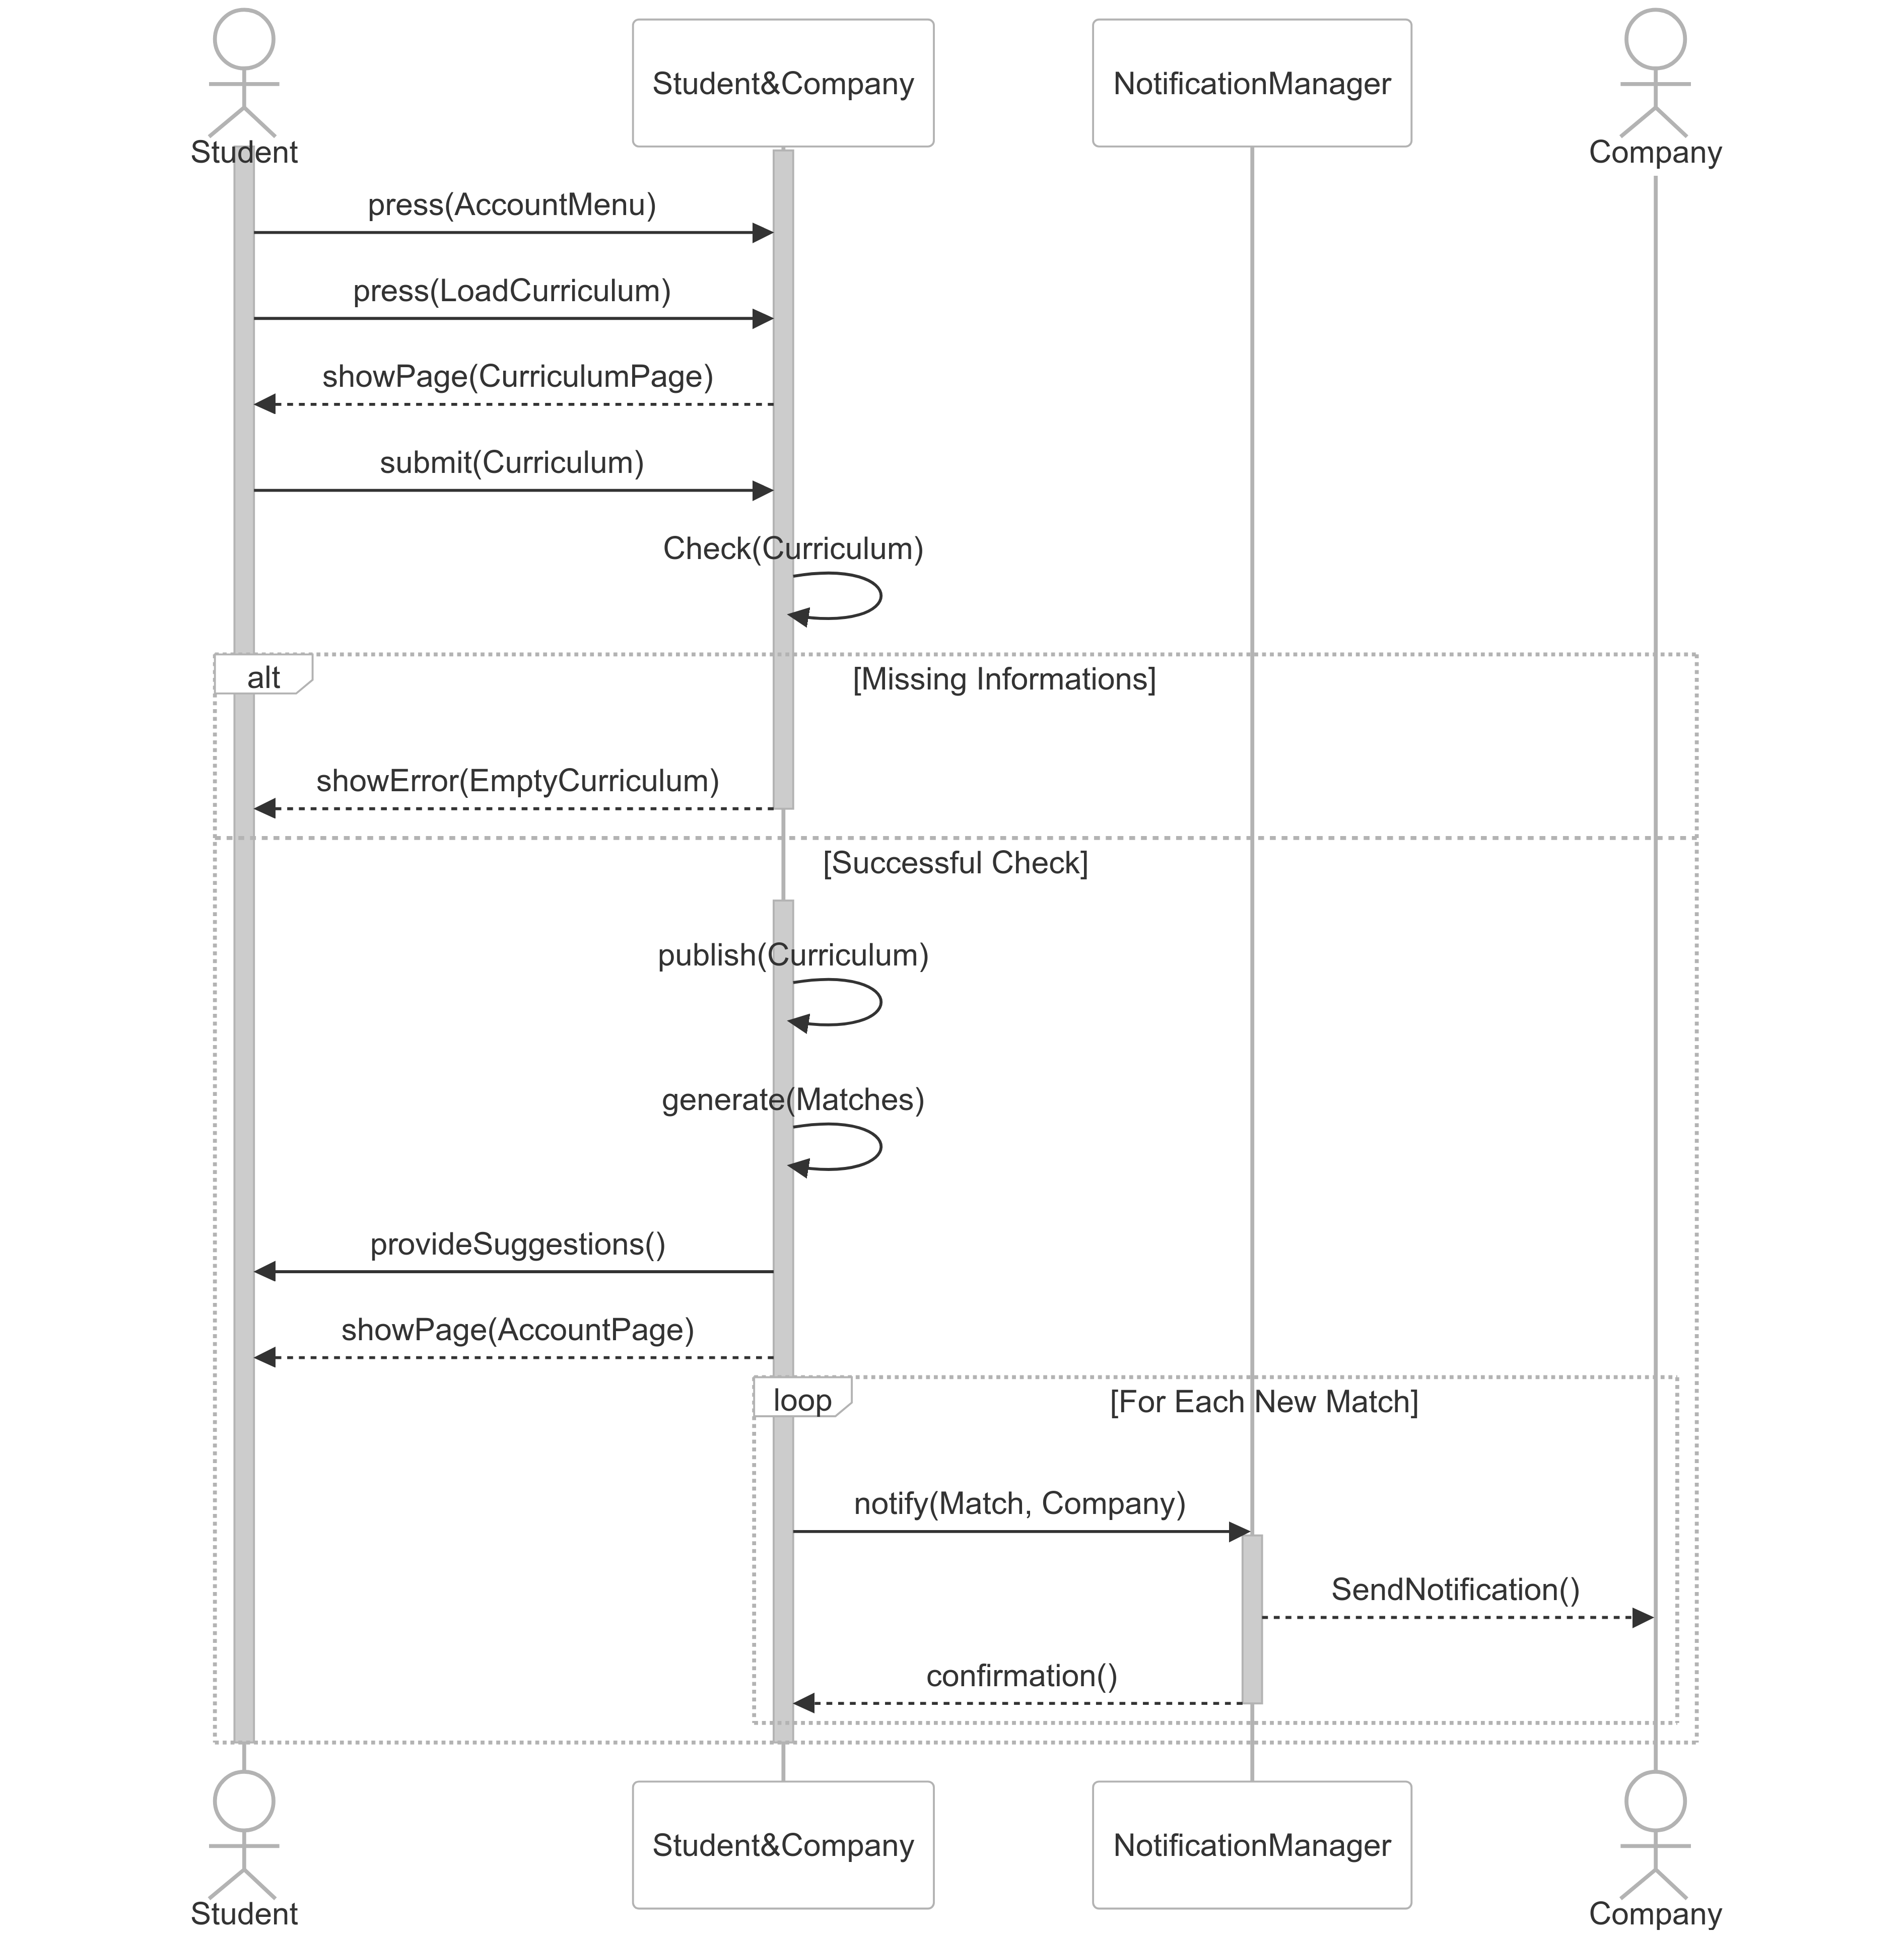
\includegraphics[width=0.8\textwidth]{Latex/Images/LoadCurriculumSequenceDiagram.png}
    \caption{[SD5]: Load Curriculum Sequence Diagram}
    \label{fig:SD5}
\end{figure}
\clearpage

\begin{figure}
    \centering
    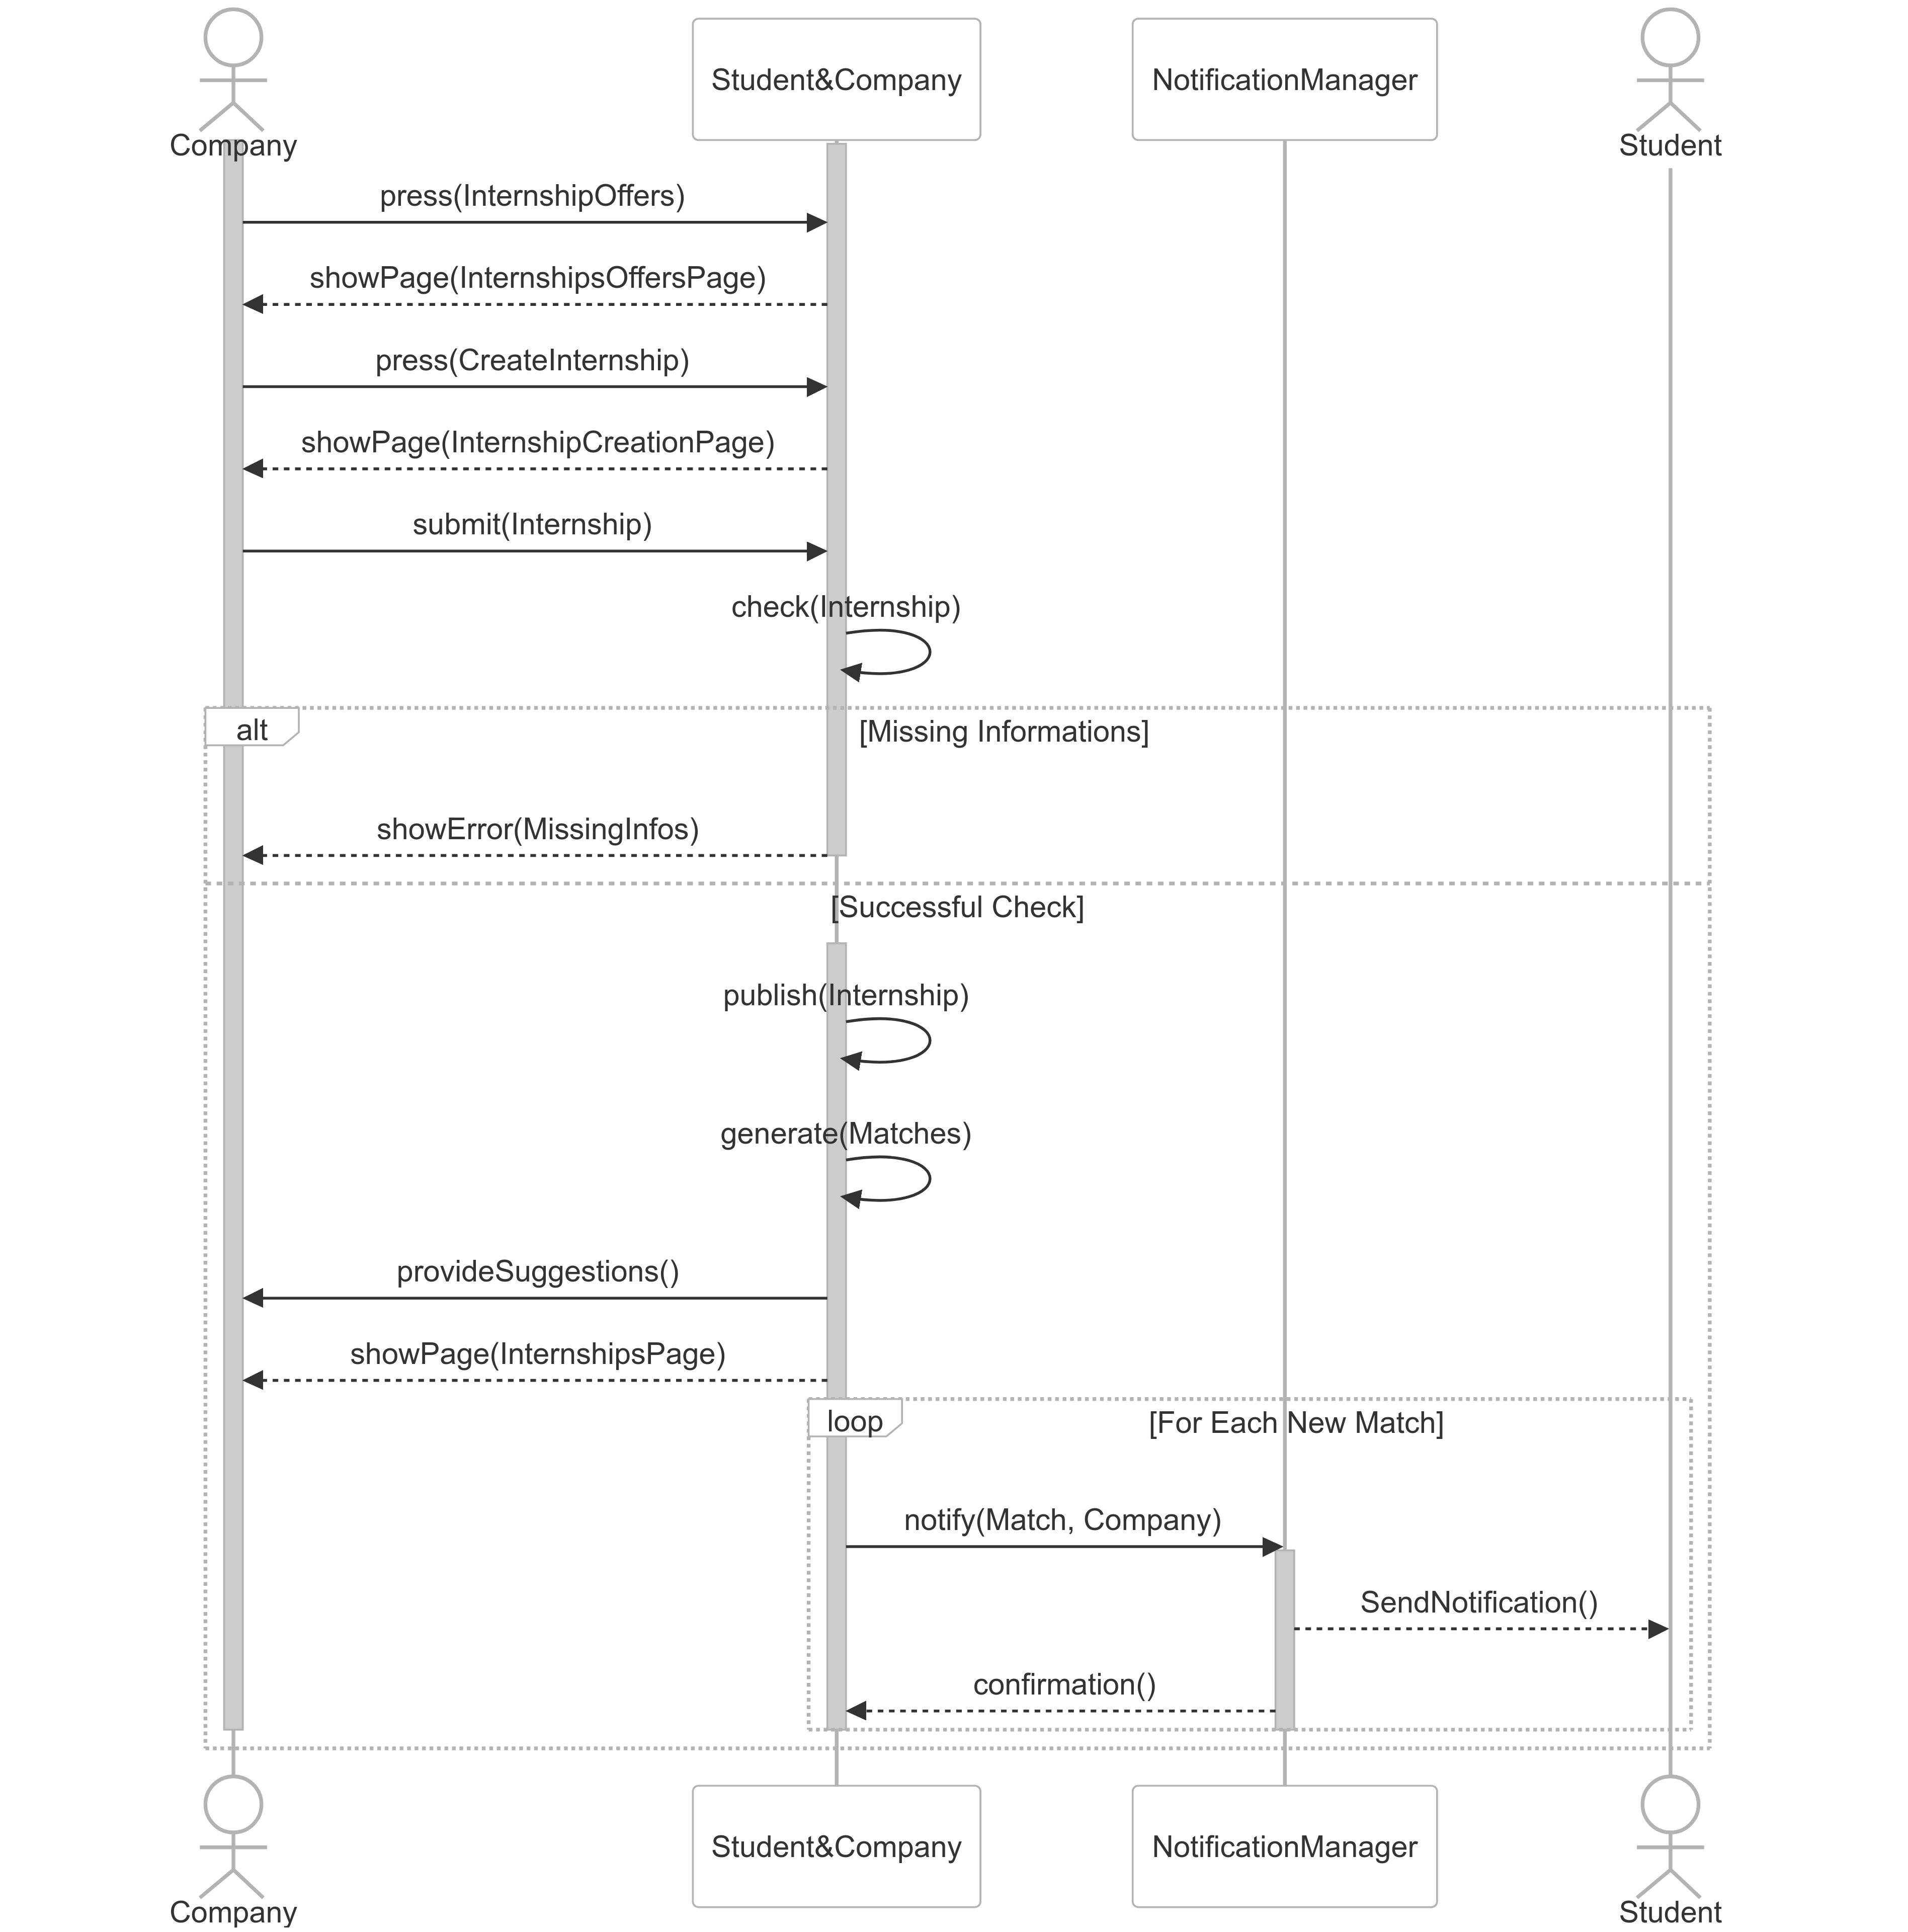
\includegraphics[width=0.8\textwidth]{Latex/Images/AdvertiseInternshipSequenceDiagram.png}
    \caption{[SD6]: Advertise Internship Sequence Diagram}
    \label{fig:SD6}
\end{figure}
\clearpage

\begin{figure}
    \centering
    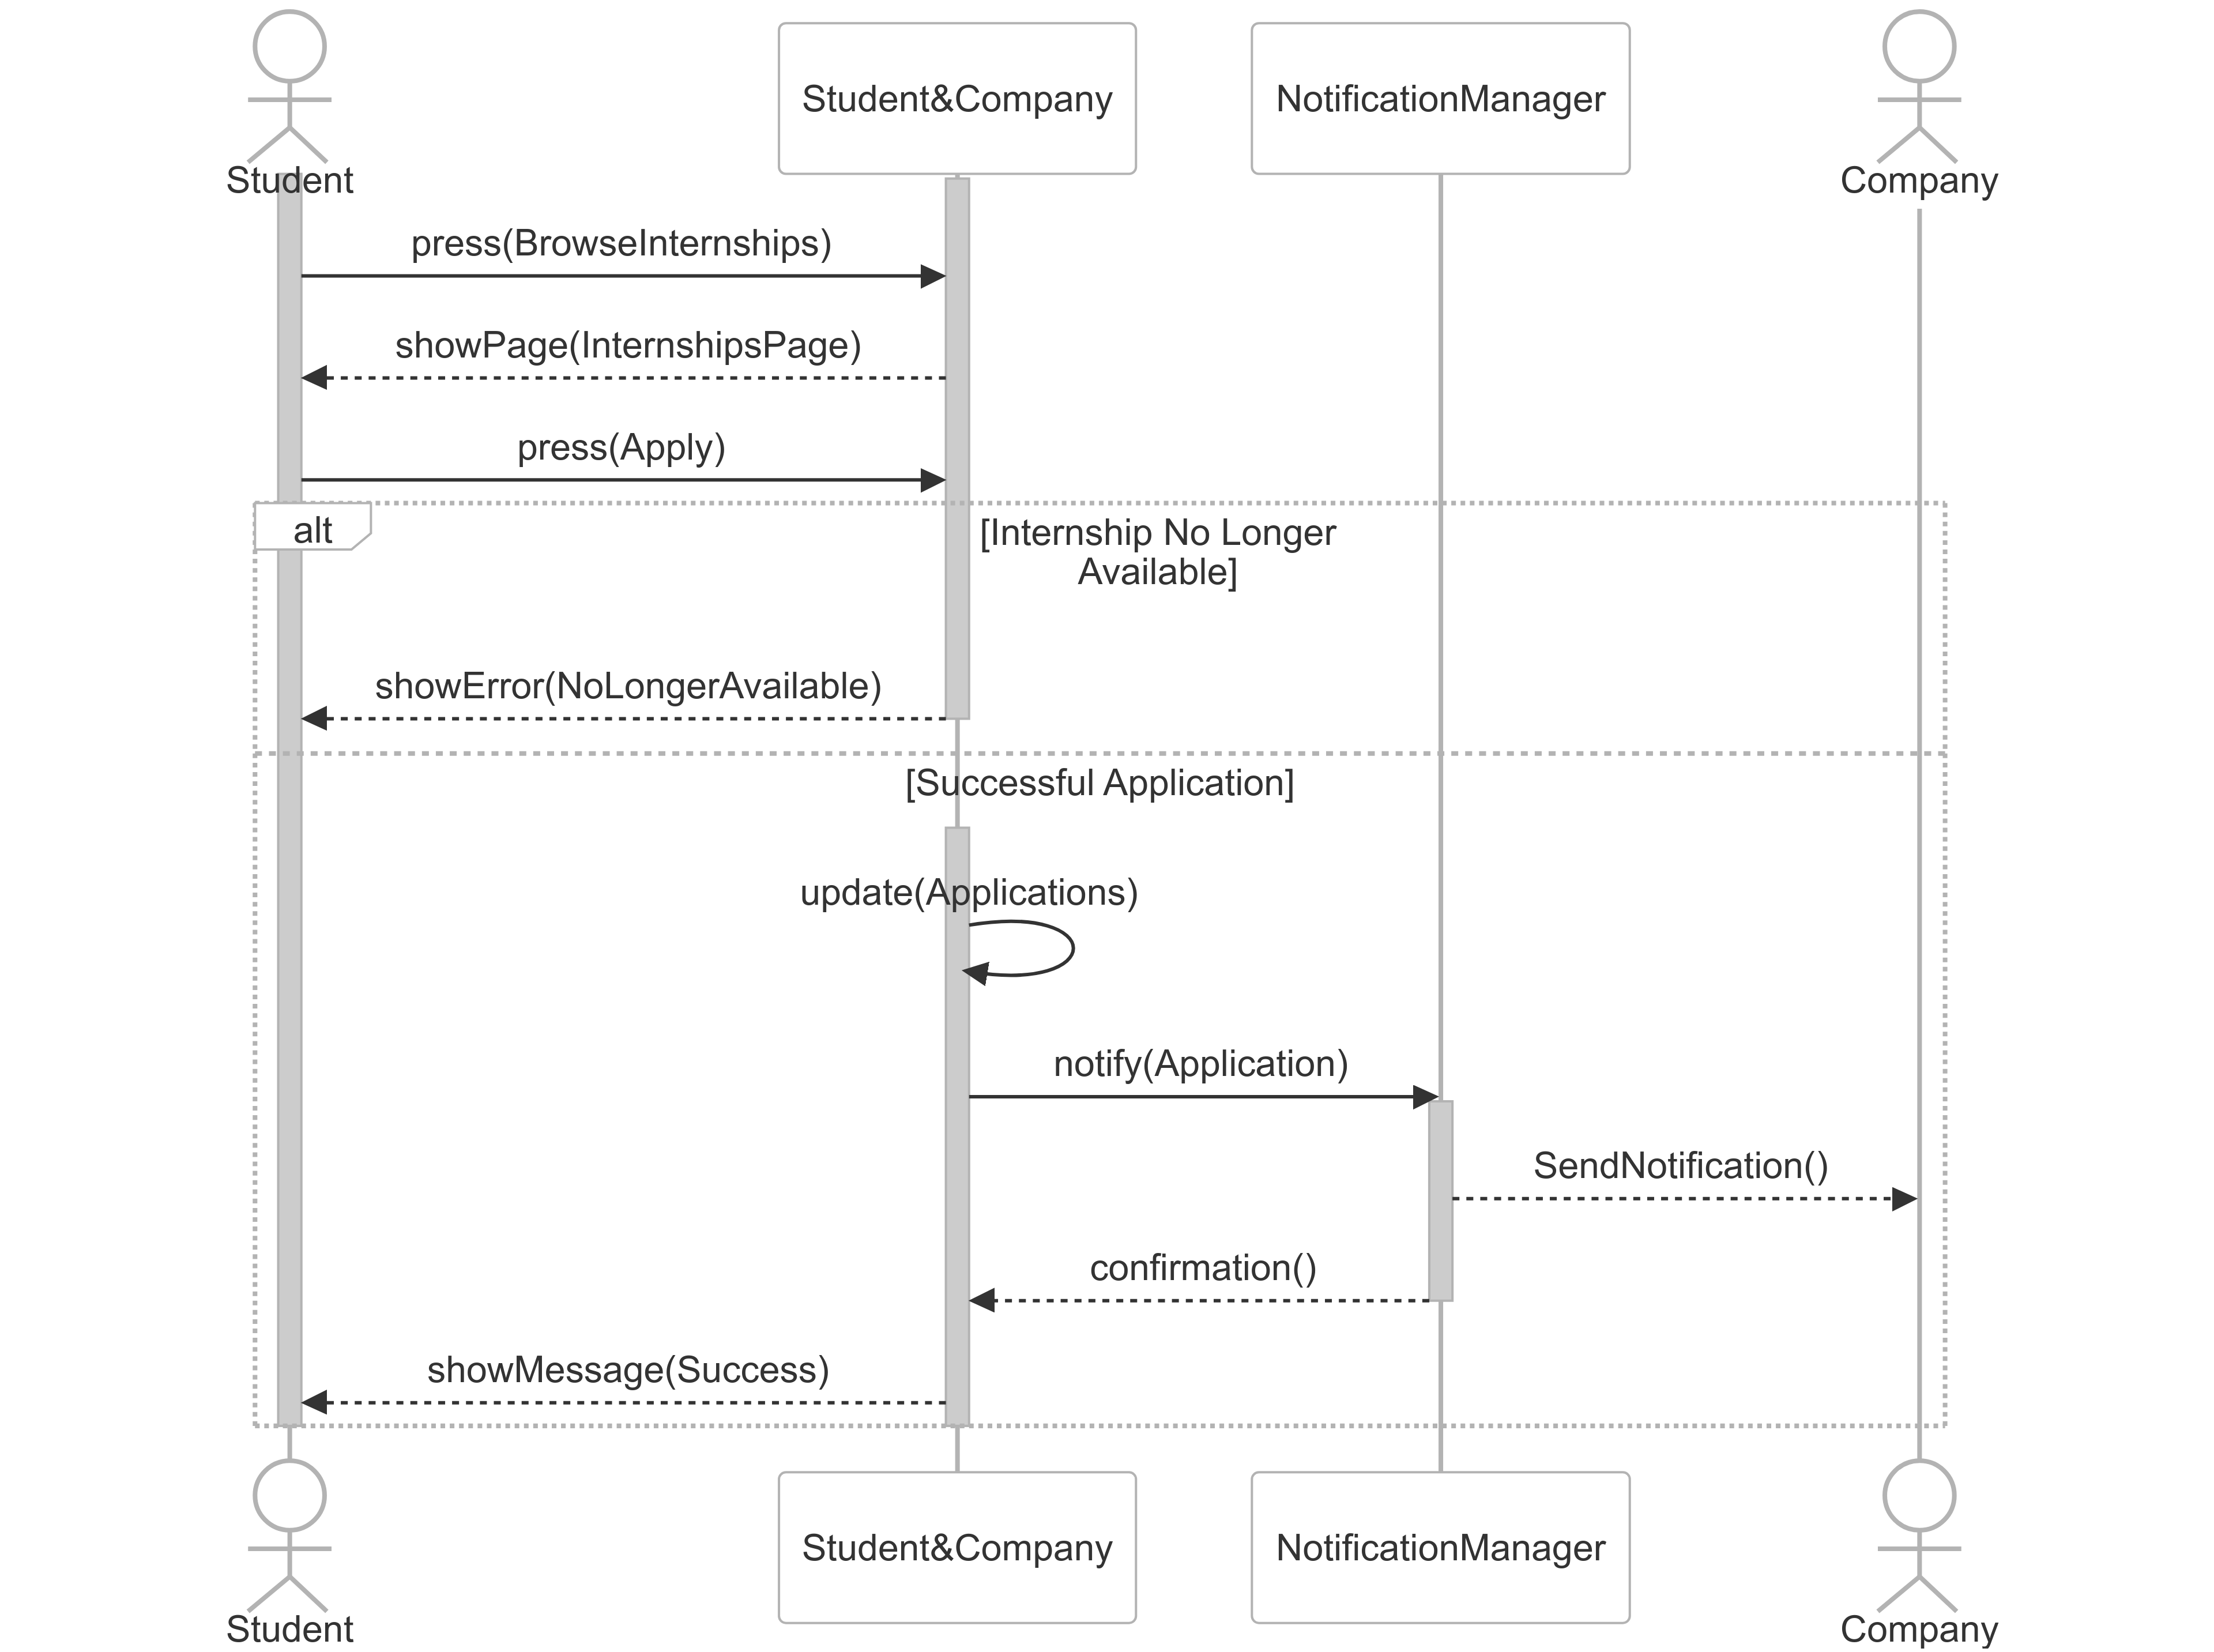
\includegraphics[width=0.8\textwidth]{Latex/Images/SpontaneousApplicationSequenceDiagram.png}
    \caption{[SD7]: Spontaneous Application Sequence Diagram}
    \label{fig:SD7}
\end{figure}

\begin{figure}
    \centering
    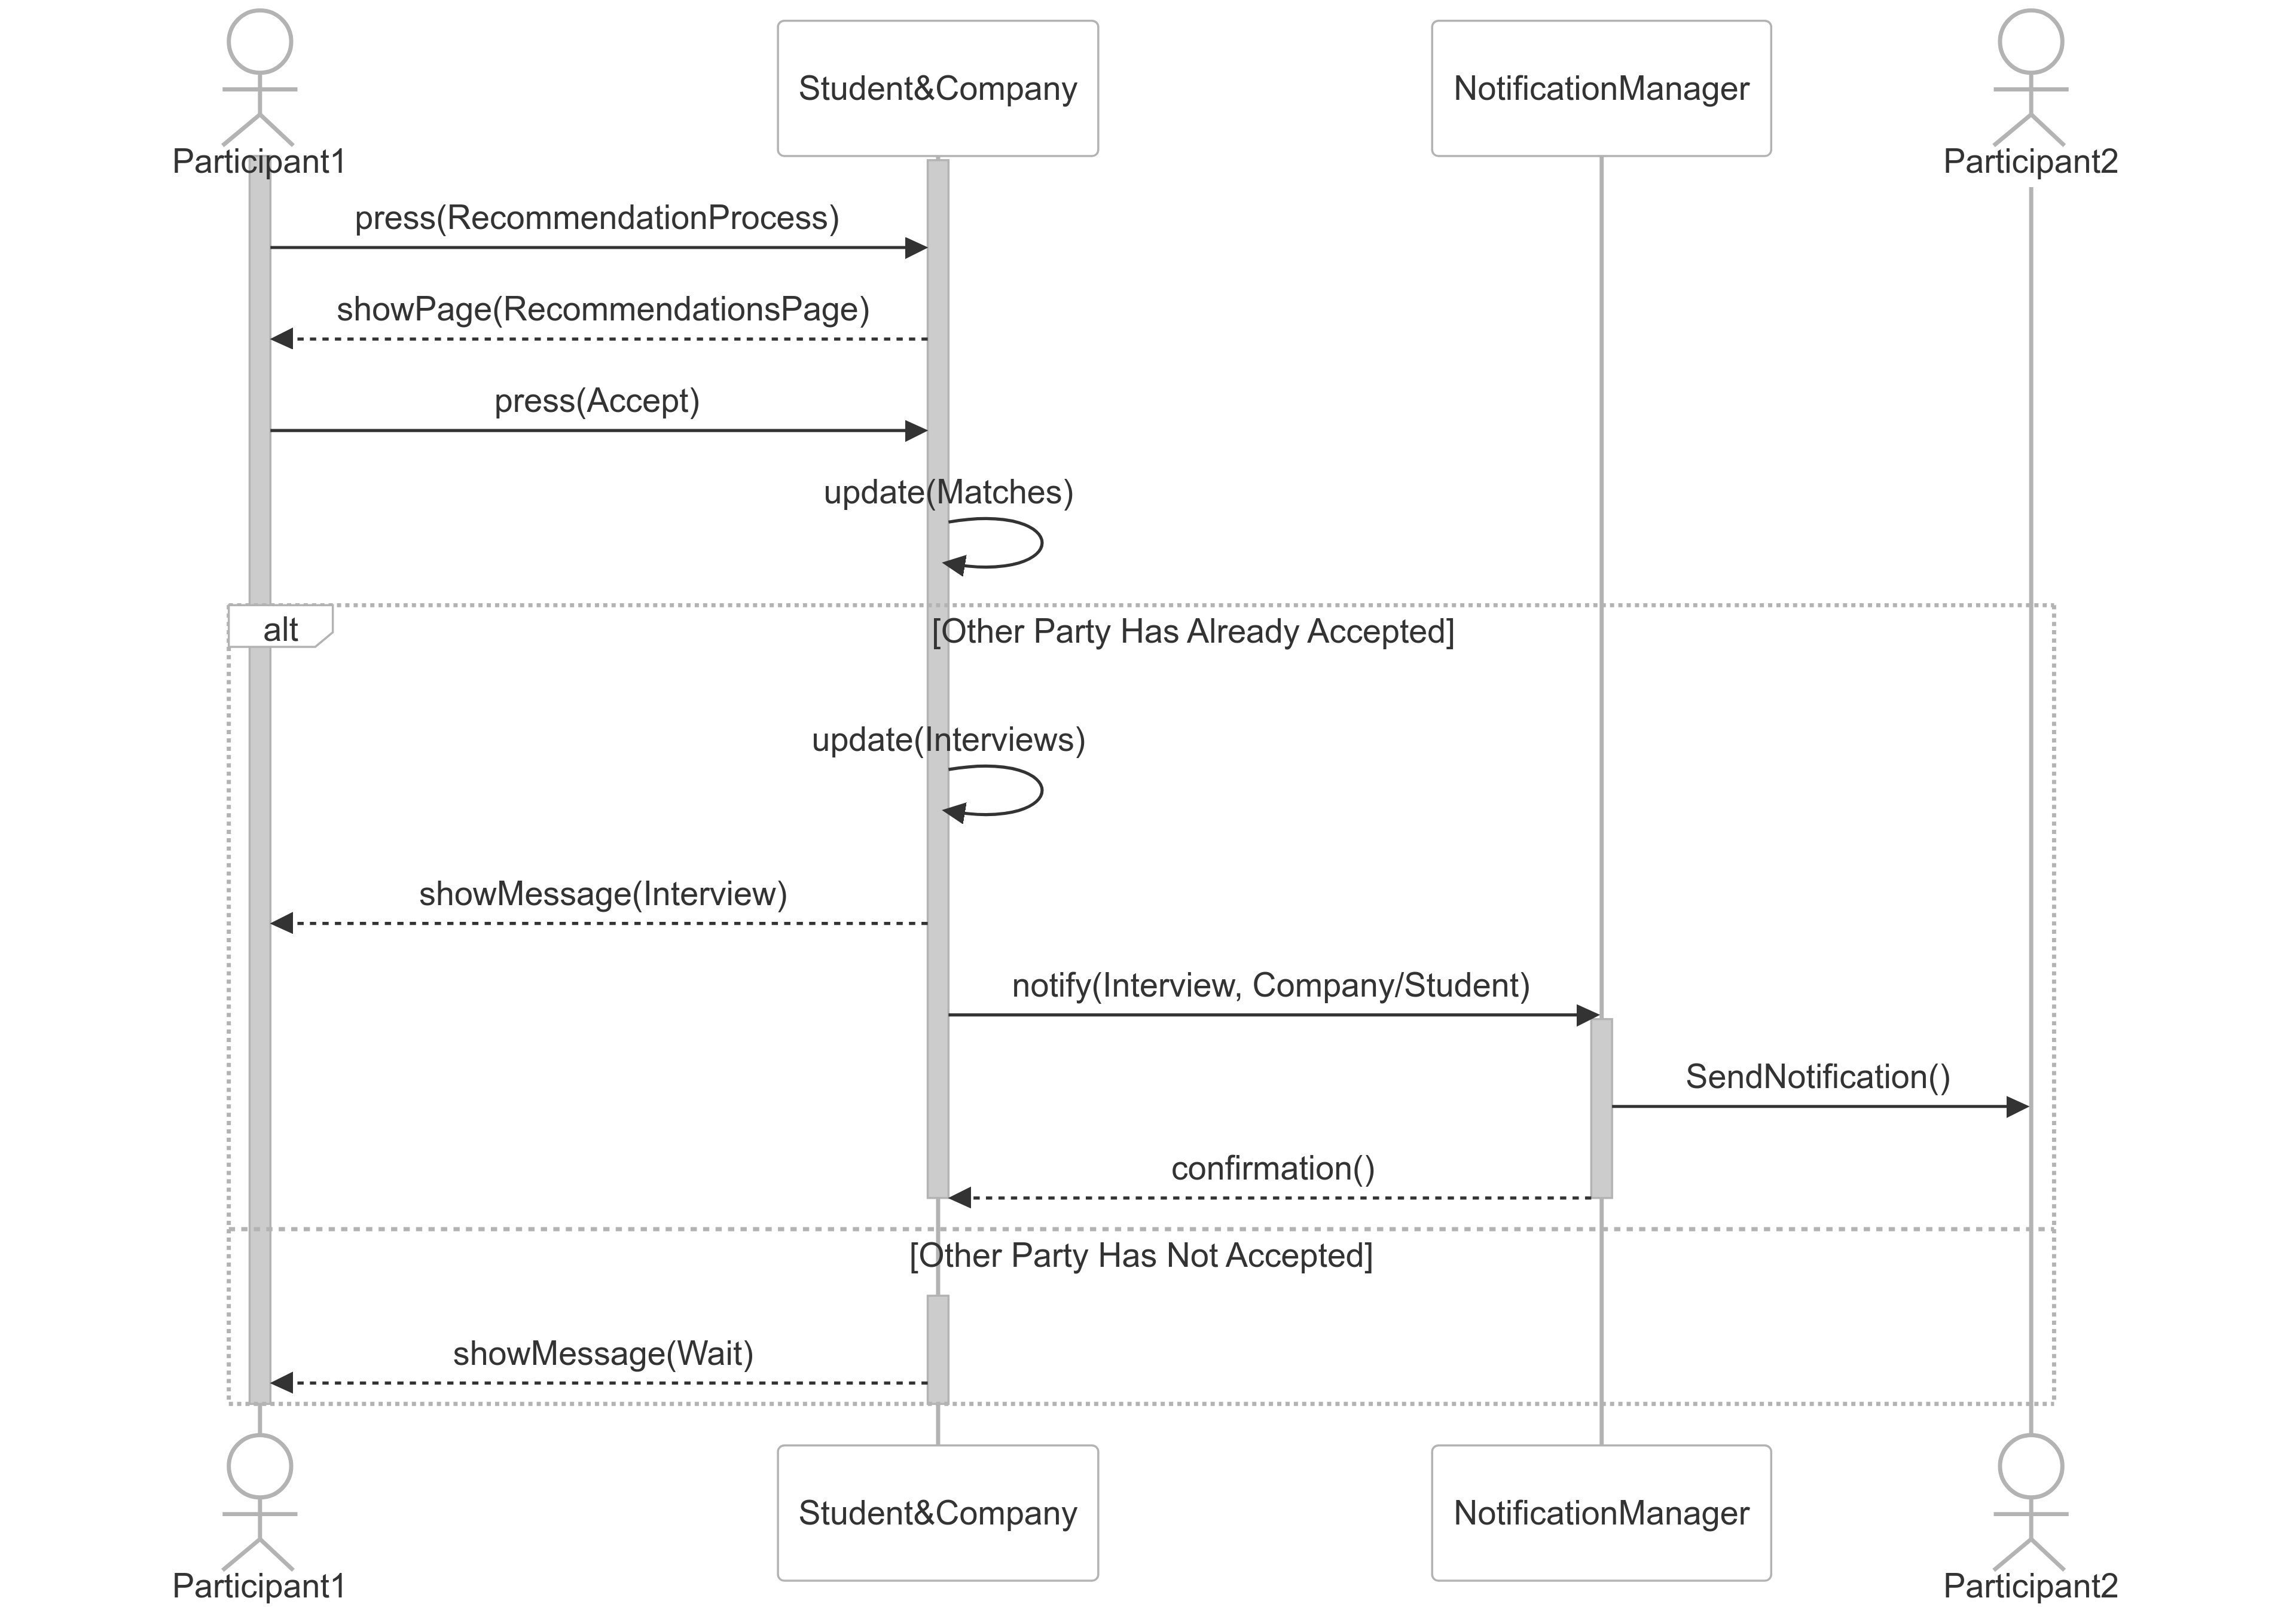
\includegraphics[width=0.8\textwidth]{Latex/Images/AcceptMatchSequenceDiagram.png}
    \caption{[SD8]: Accept Match Sequence Diagram}
    \label{fig:SD8}
\end{figure}
\clearpage

\begin{figure}
    \centering
    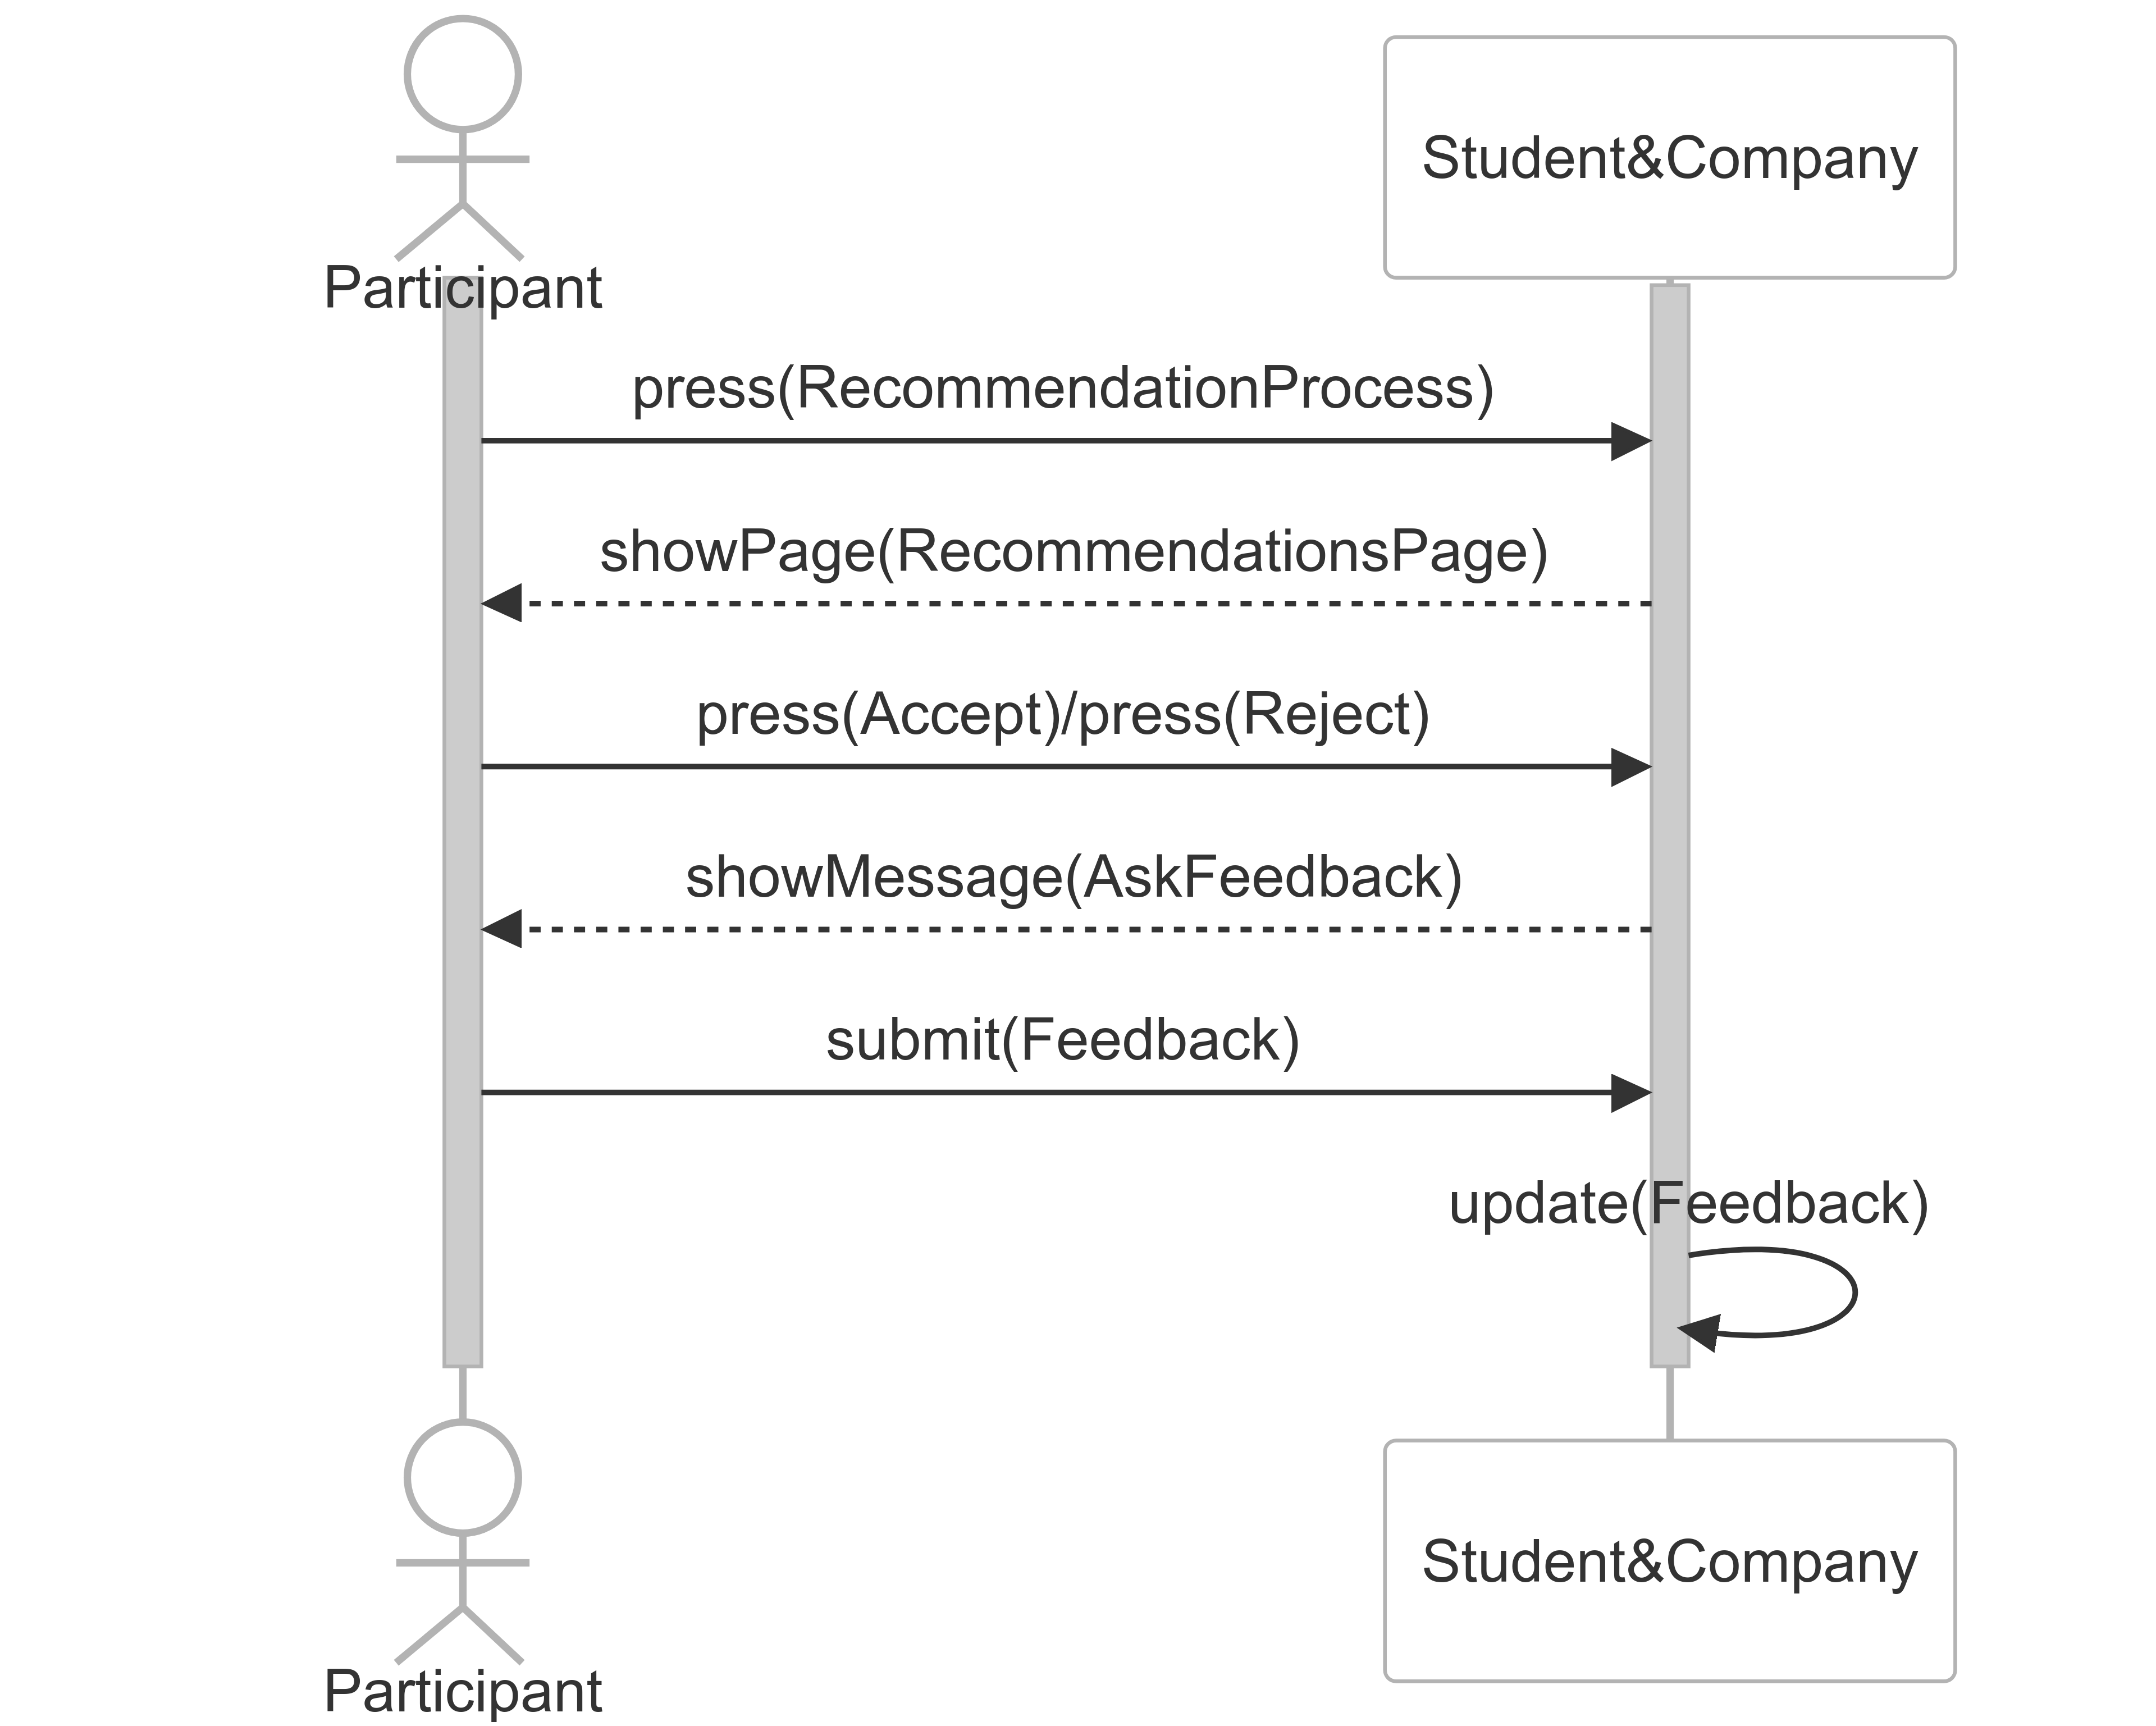
\includegraphics[width=0.55\textwidth]{Latex/Images/FeedbackMechanismSequenceDiagram.png}
    \caption{[SD9]: Feedback mechanism Sequence Diagram}
    \label{fig:SD9}
\end{figure}

\begin{figure}
    \centering
    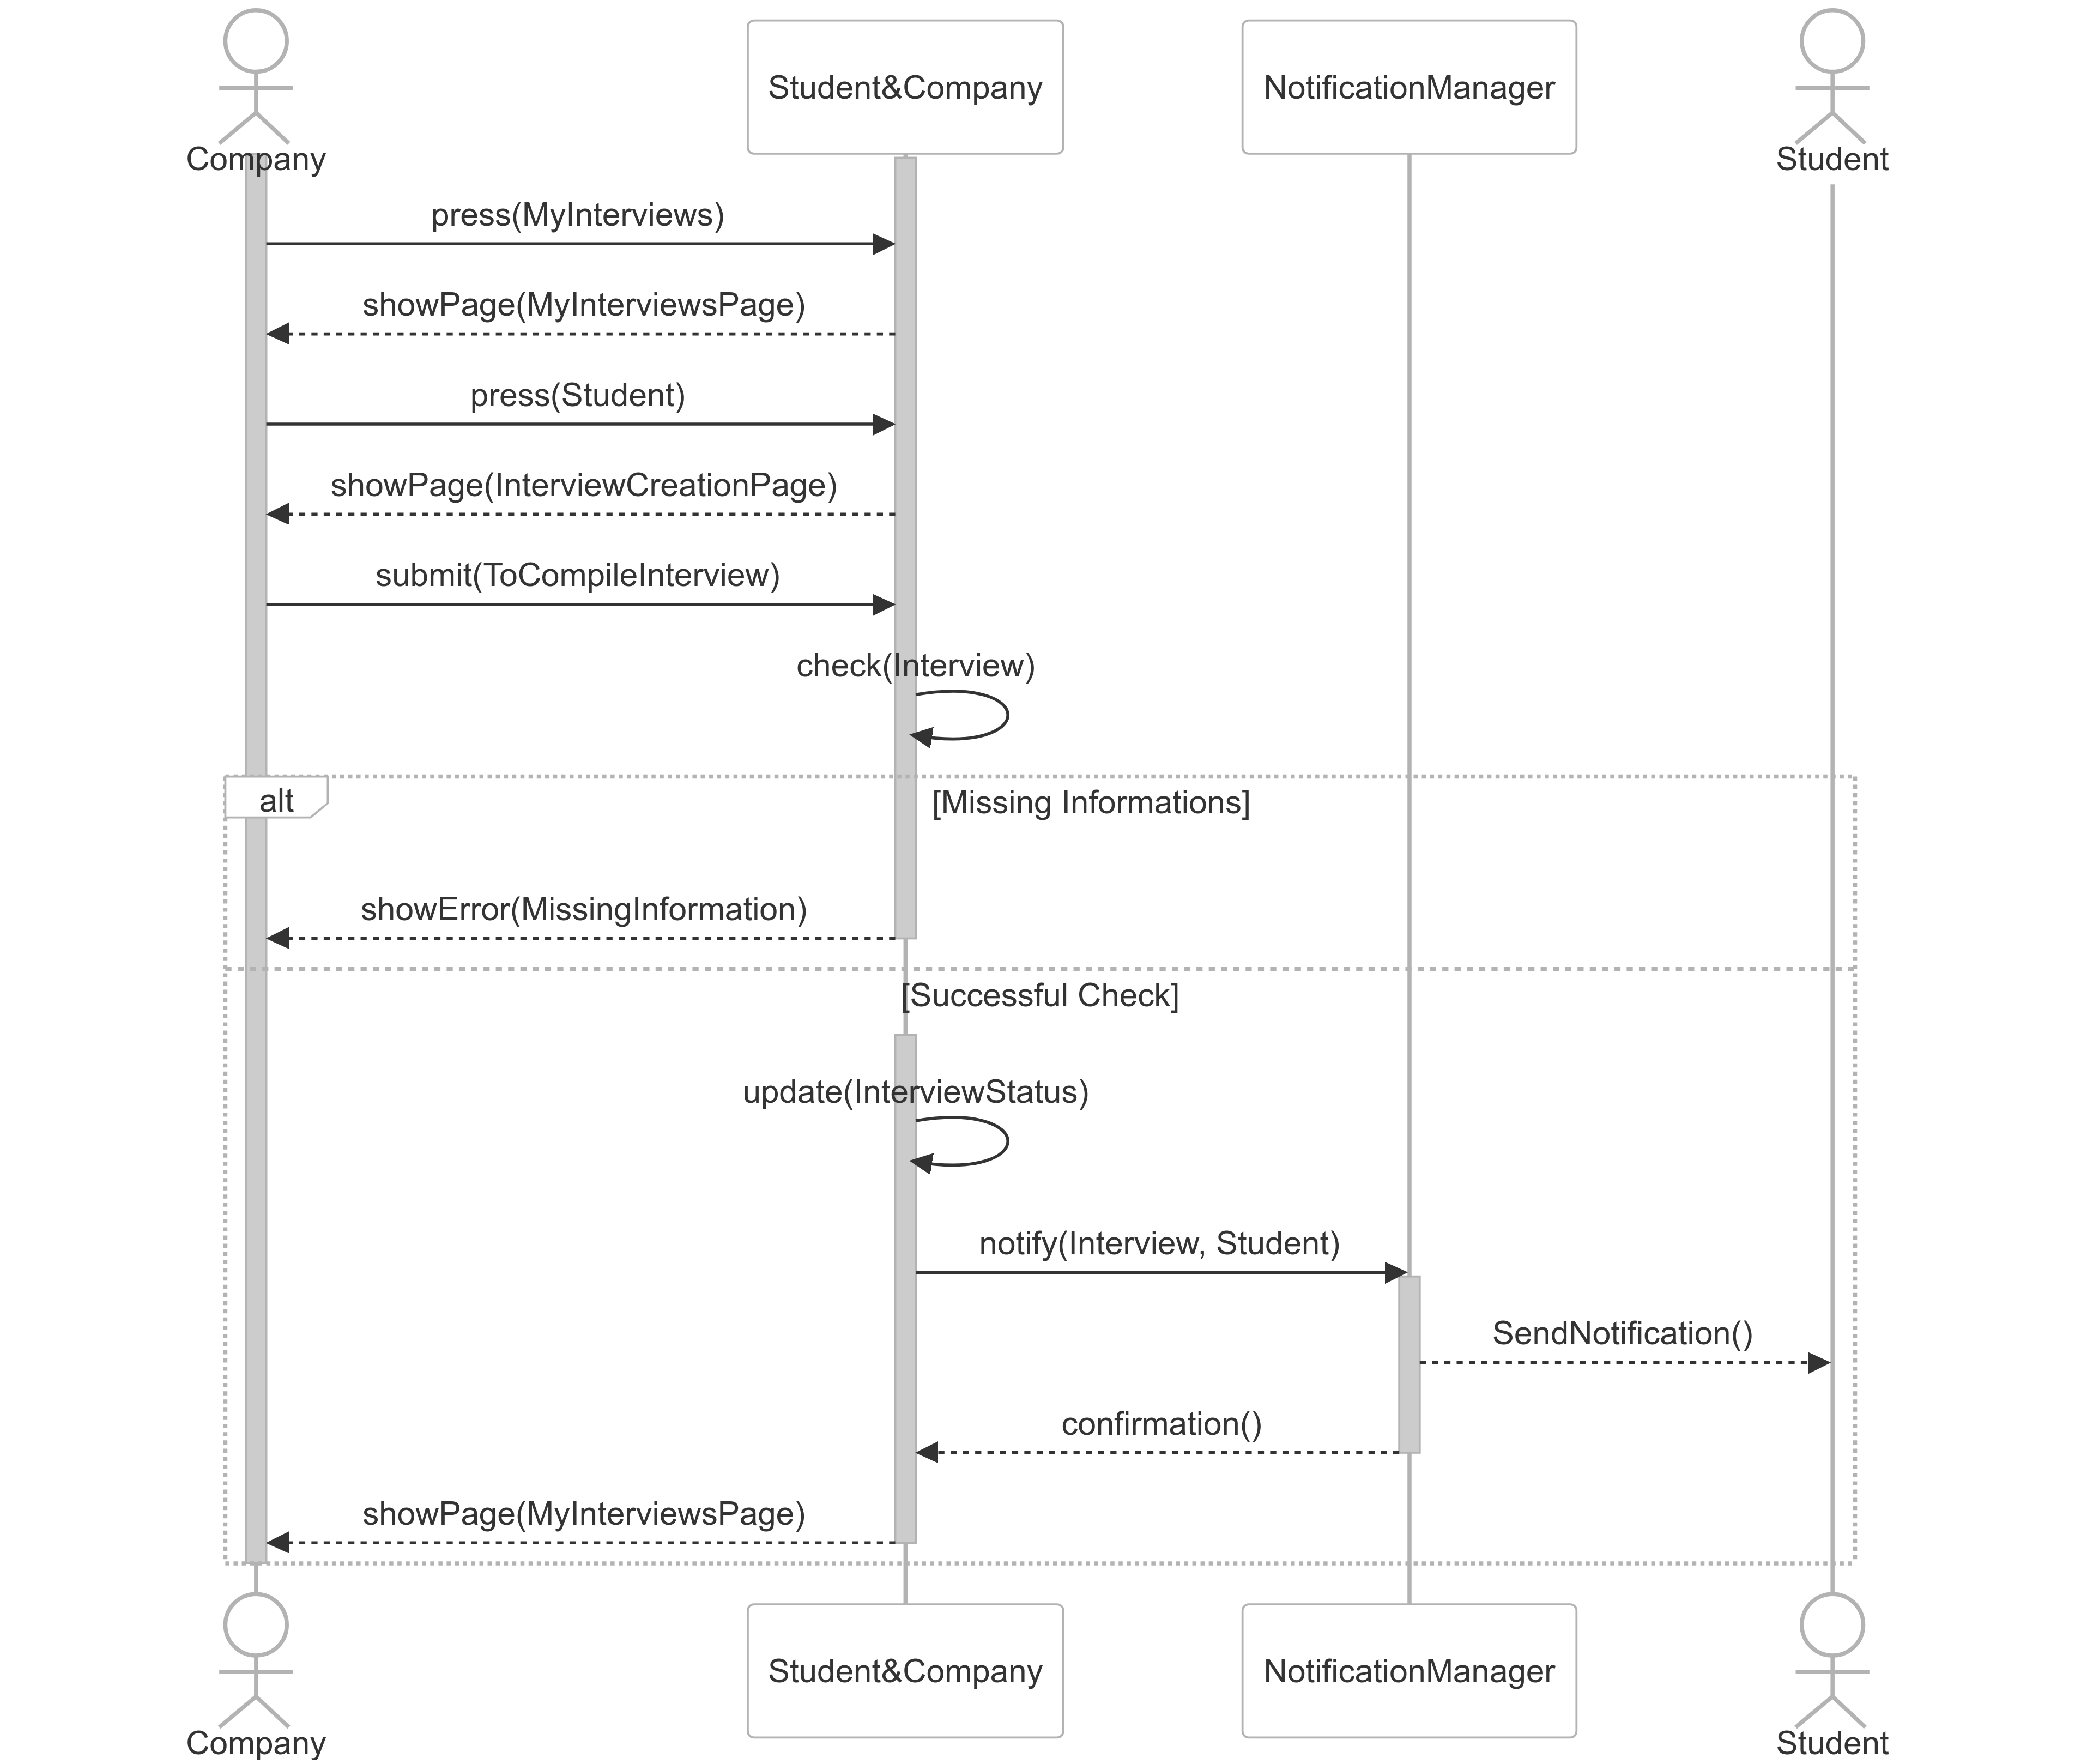
\includegraphics[width=0.8\textwidth]{Latex/Images/AssignInterviewSequenceDiagram.png}
    \caption{[SD10]: Assign Interview Sequence Diagram}
    \label{fig:SD10}
\end{figure}
\clearpage

\begin{figure}
    \centering
    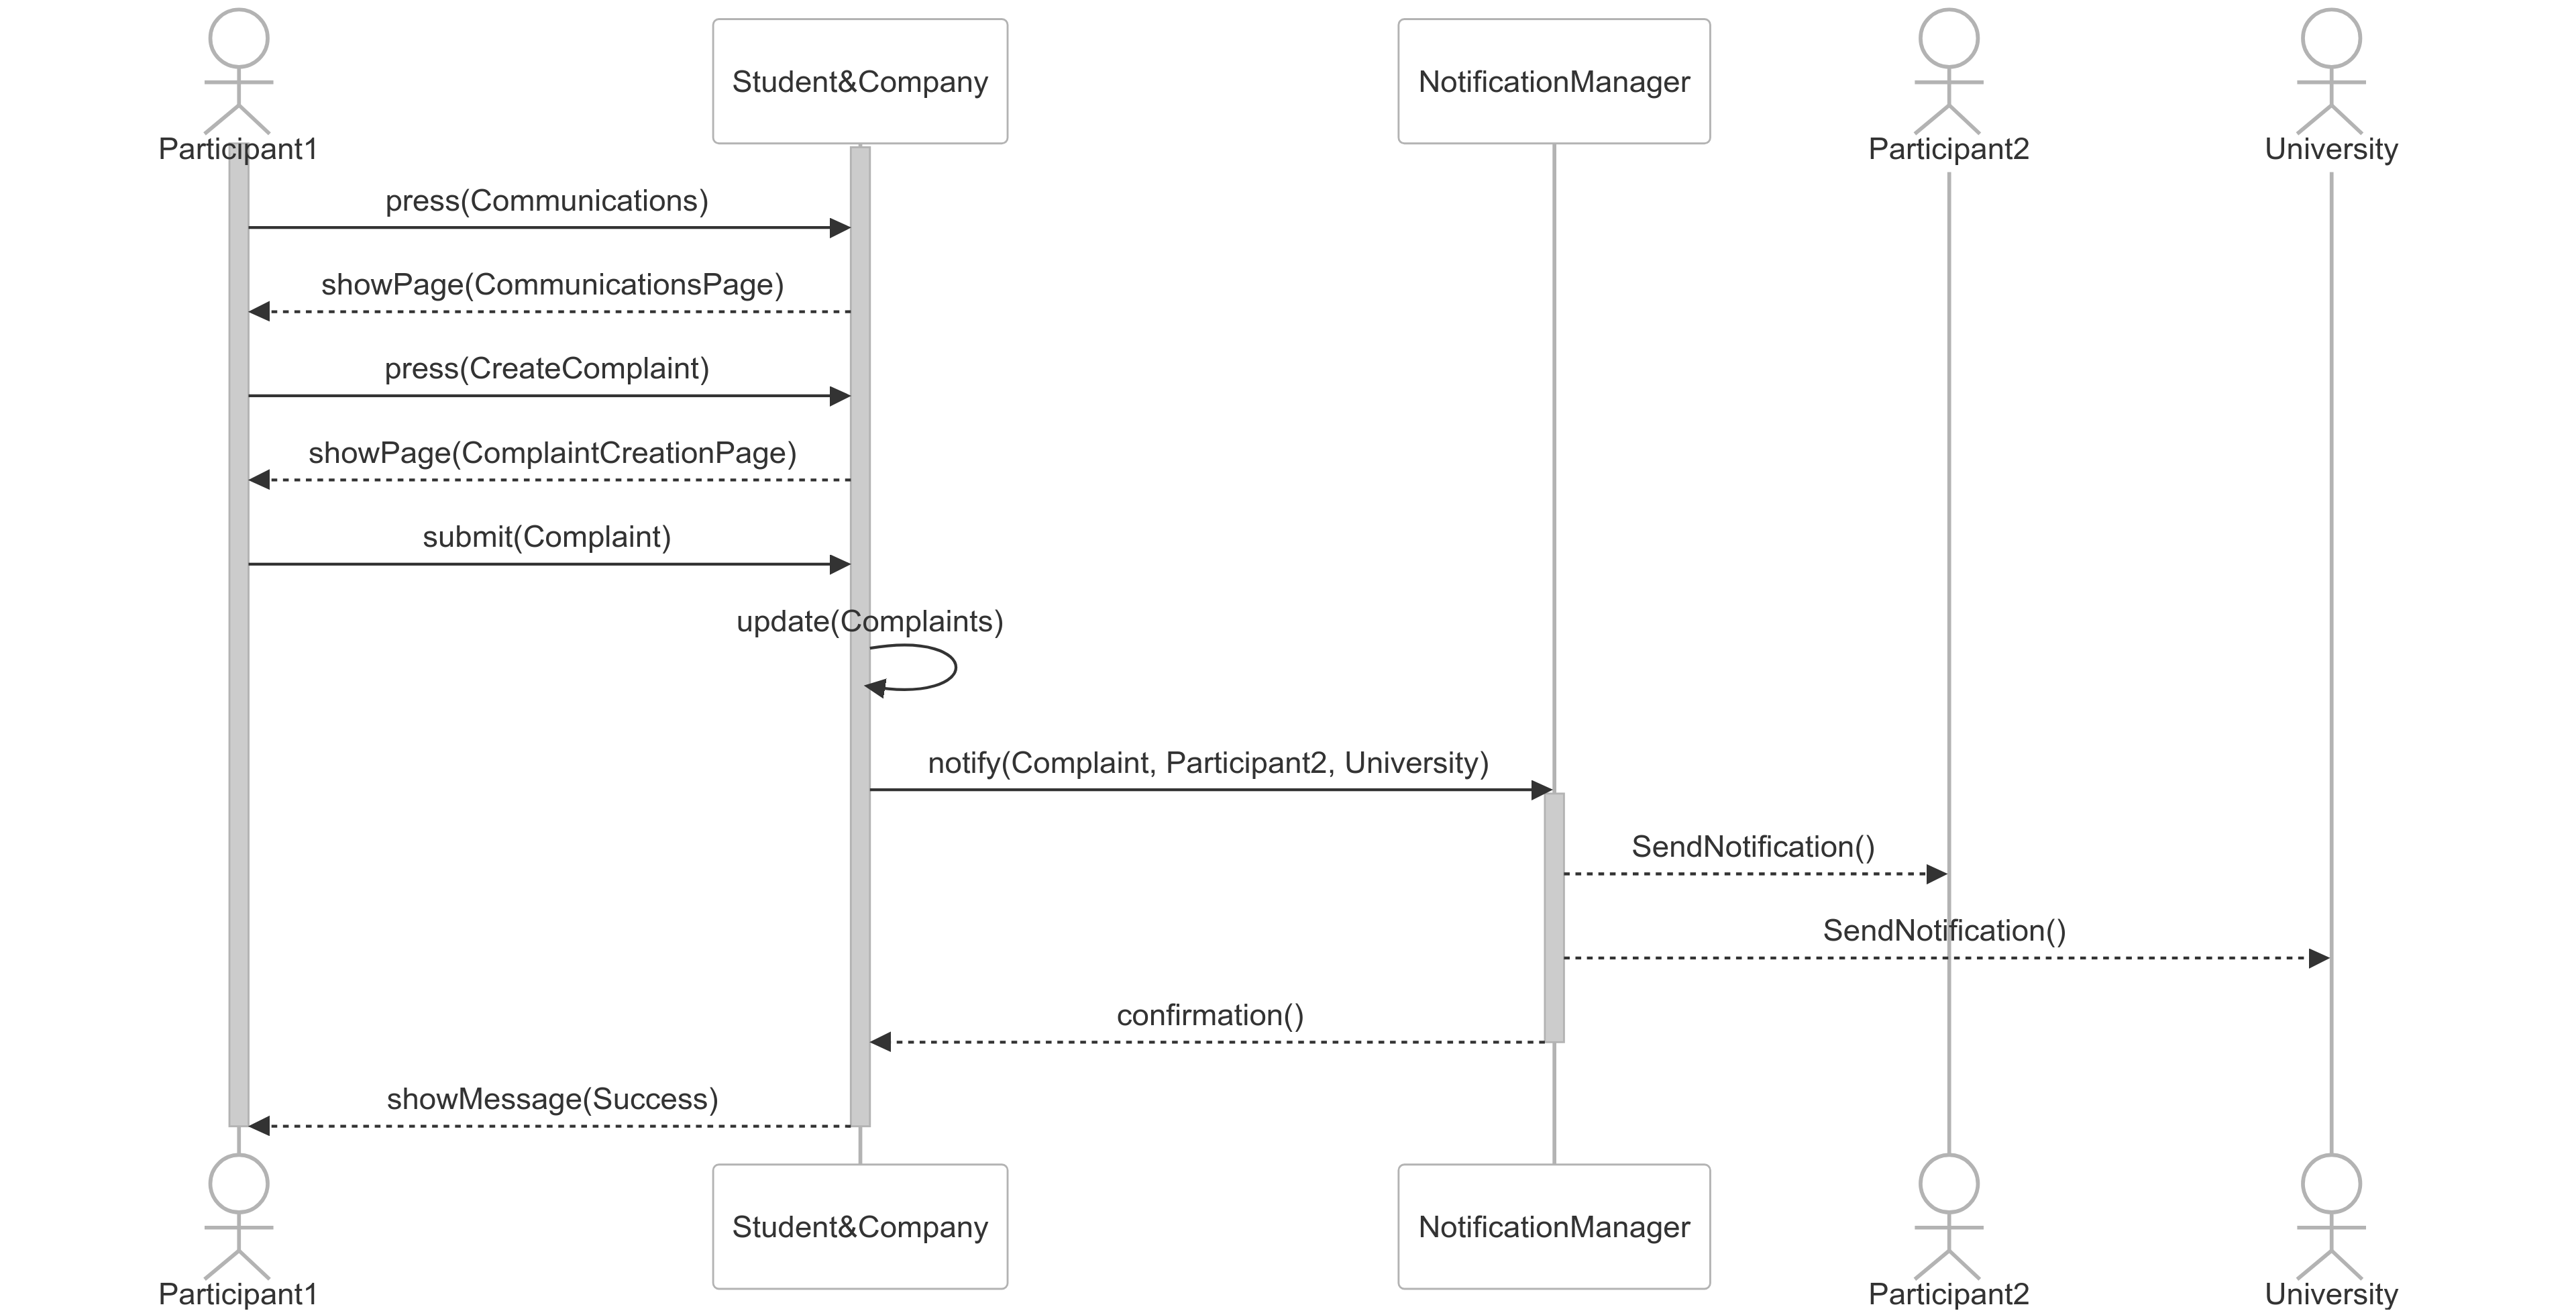
\includegraphics[width=1\textwidth]{Latex/Images/PublishComplaintSequenceDiagram.png}
    \caption{[SD11]: Publish Complaint Sequence Diagram}
    \label{fig:SD11}
\end{figure}

\begin{figure}
    \centering
    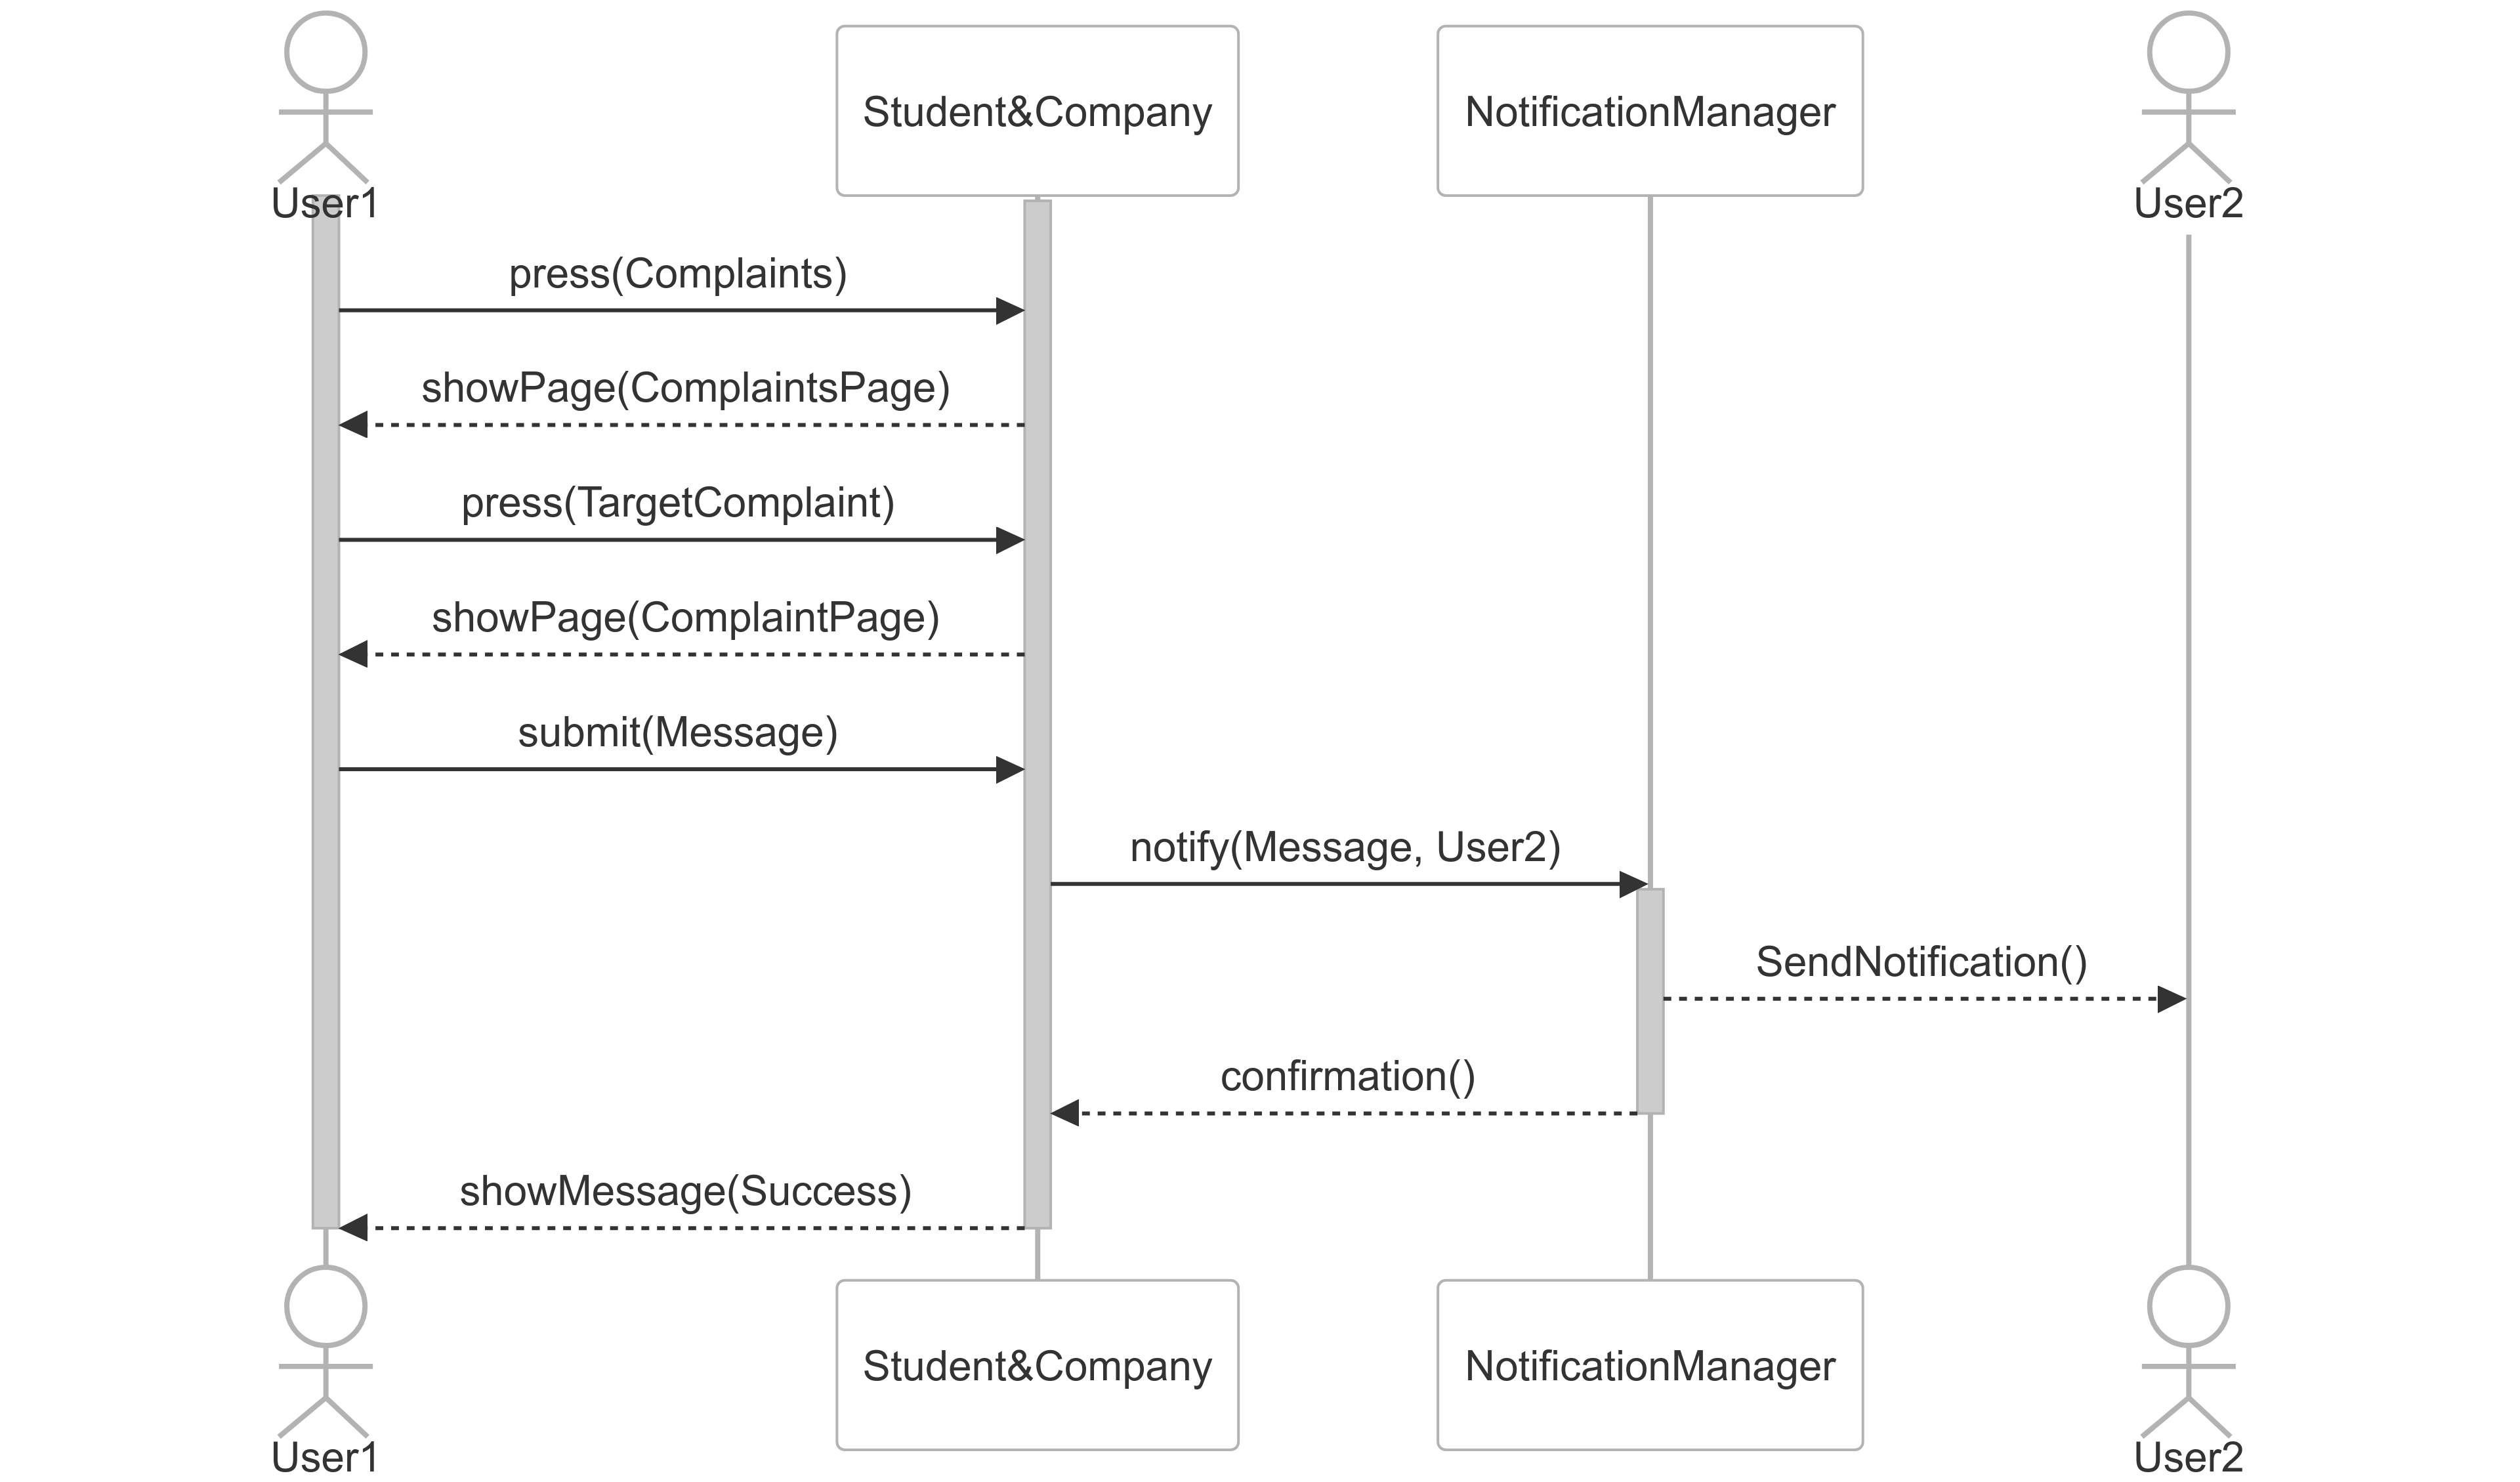
\includegraphics[width=0.7\textwidth]{Latex/Images/RespondToComplaintSequenceDiagram.png}
    \caption{[SD12]: Respond to Complaint Sequence Diagram}
    \label{fig:SD12}
\end{figure}

\begin{figure}
    \centering
    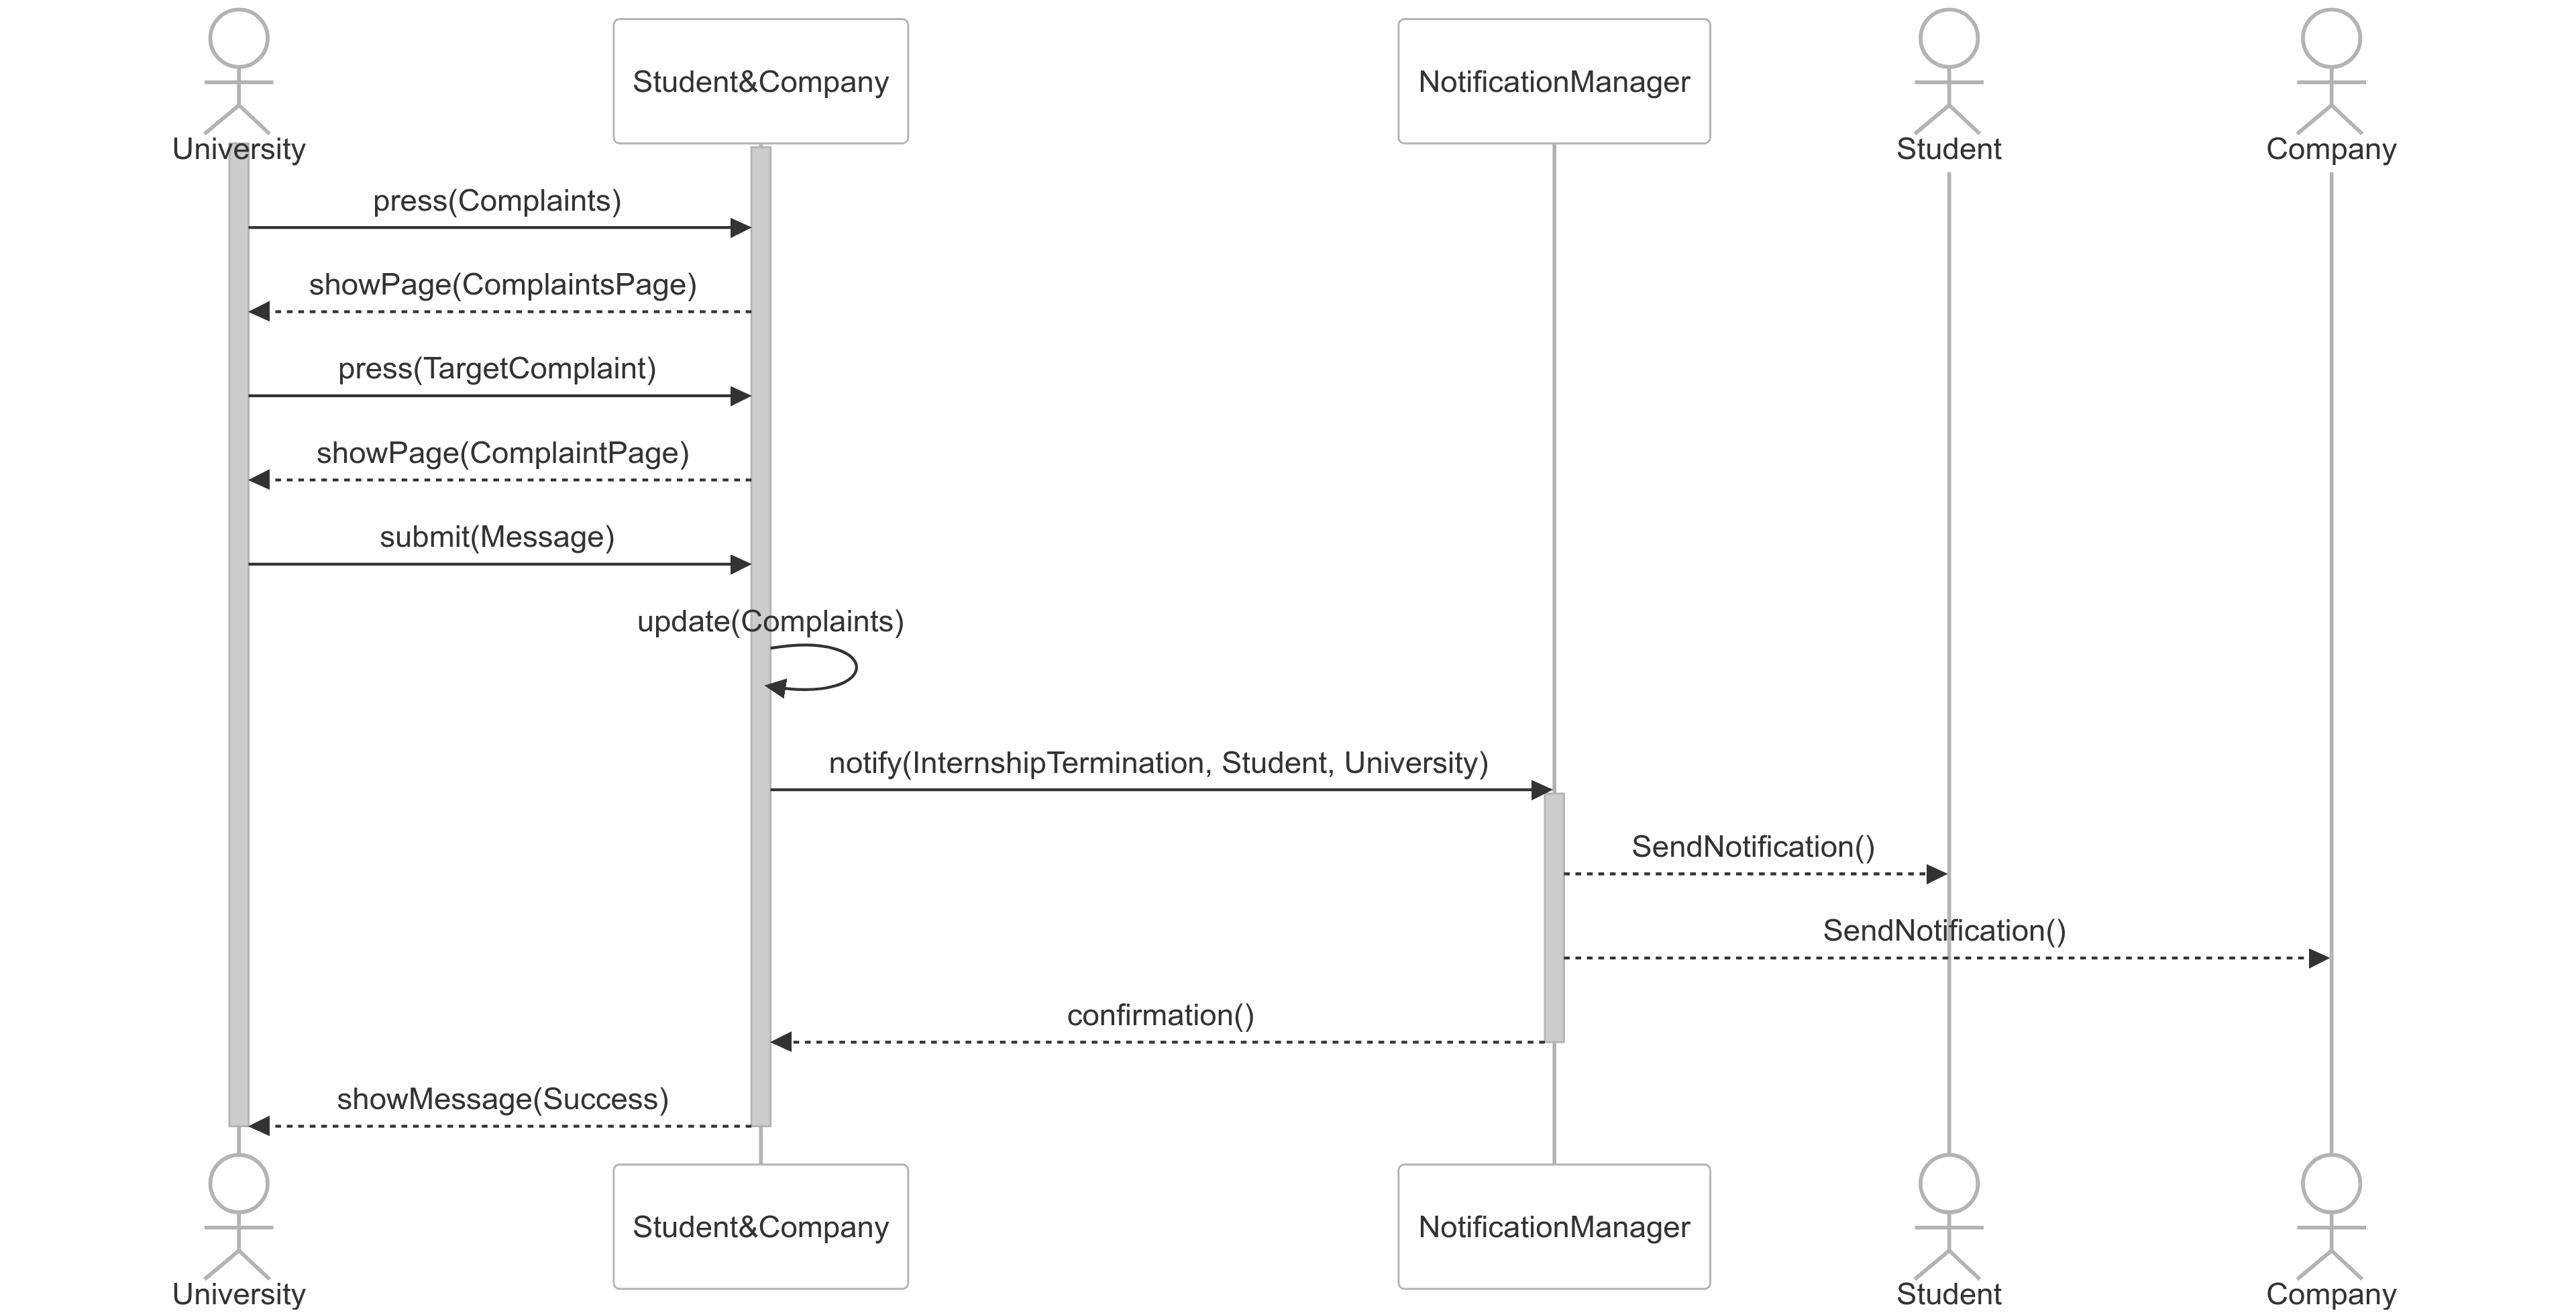
\includegraphics[width=1\textwidth]{Latex/Images/HandleComplaintSequenceDiagram.png}
    \caption{[SD13]: Handle Complaint Sequence Diagram}
    \label{fig:SD13}
\end{figure}

\begin{figure}
    \centering
    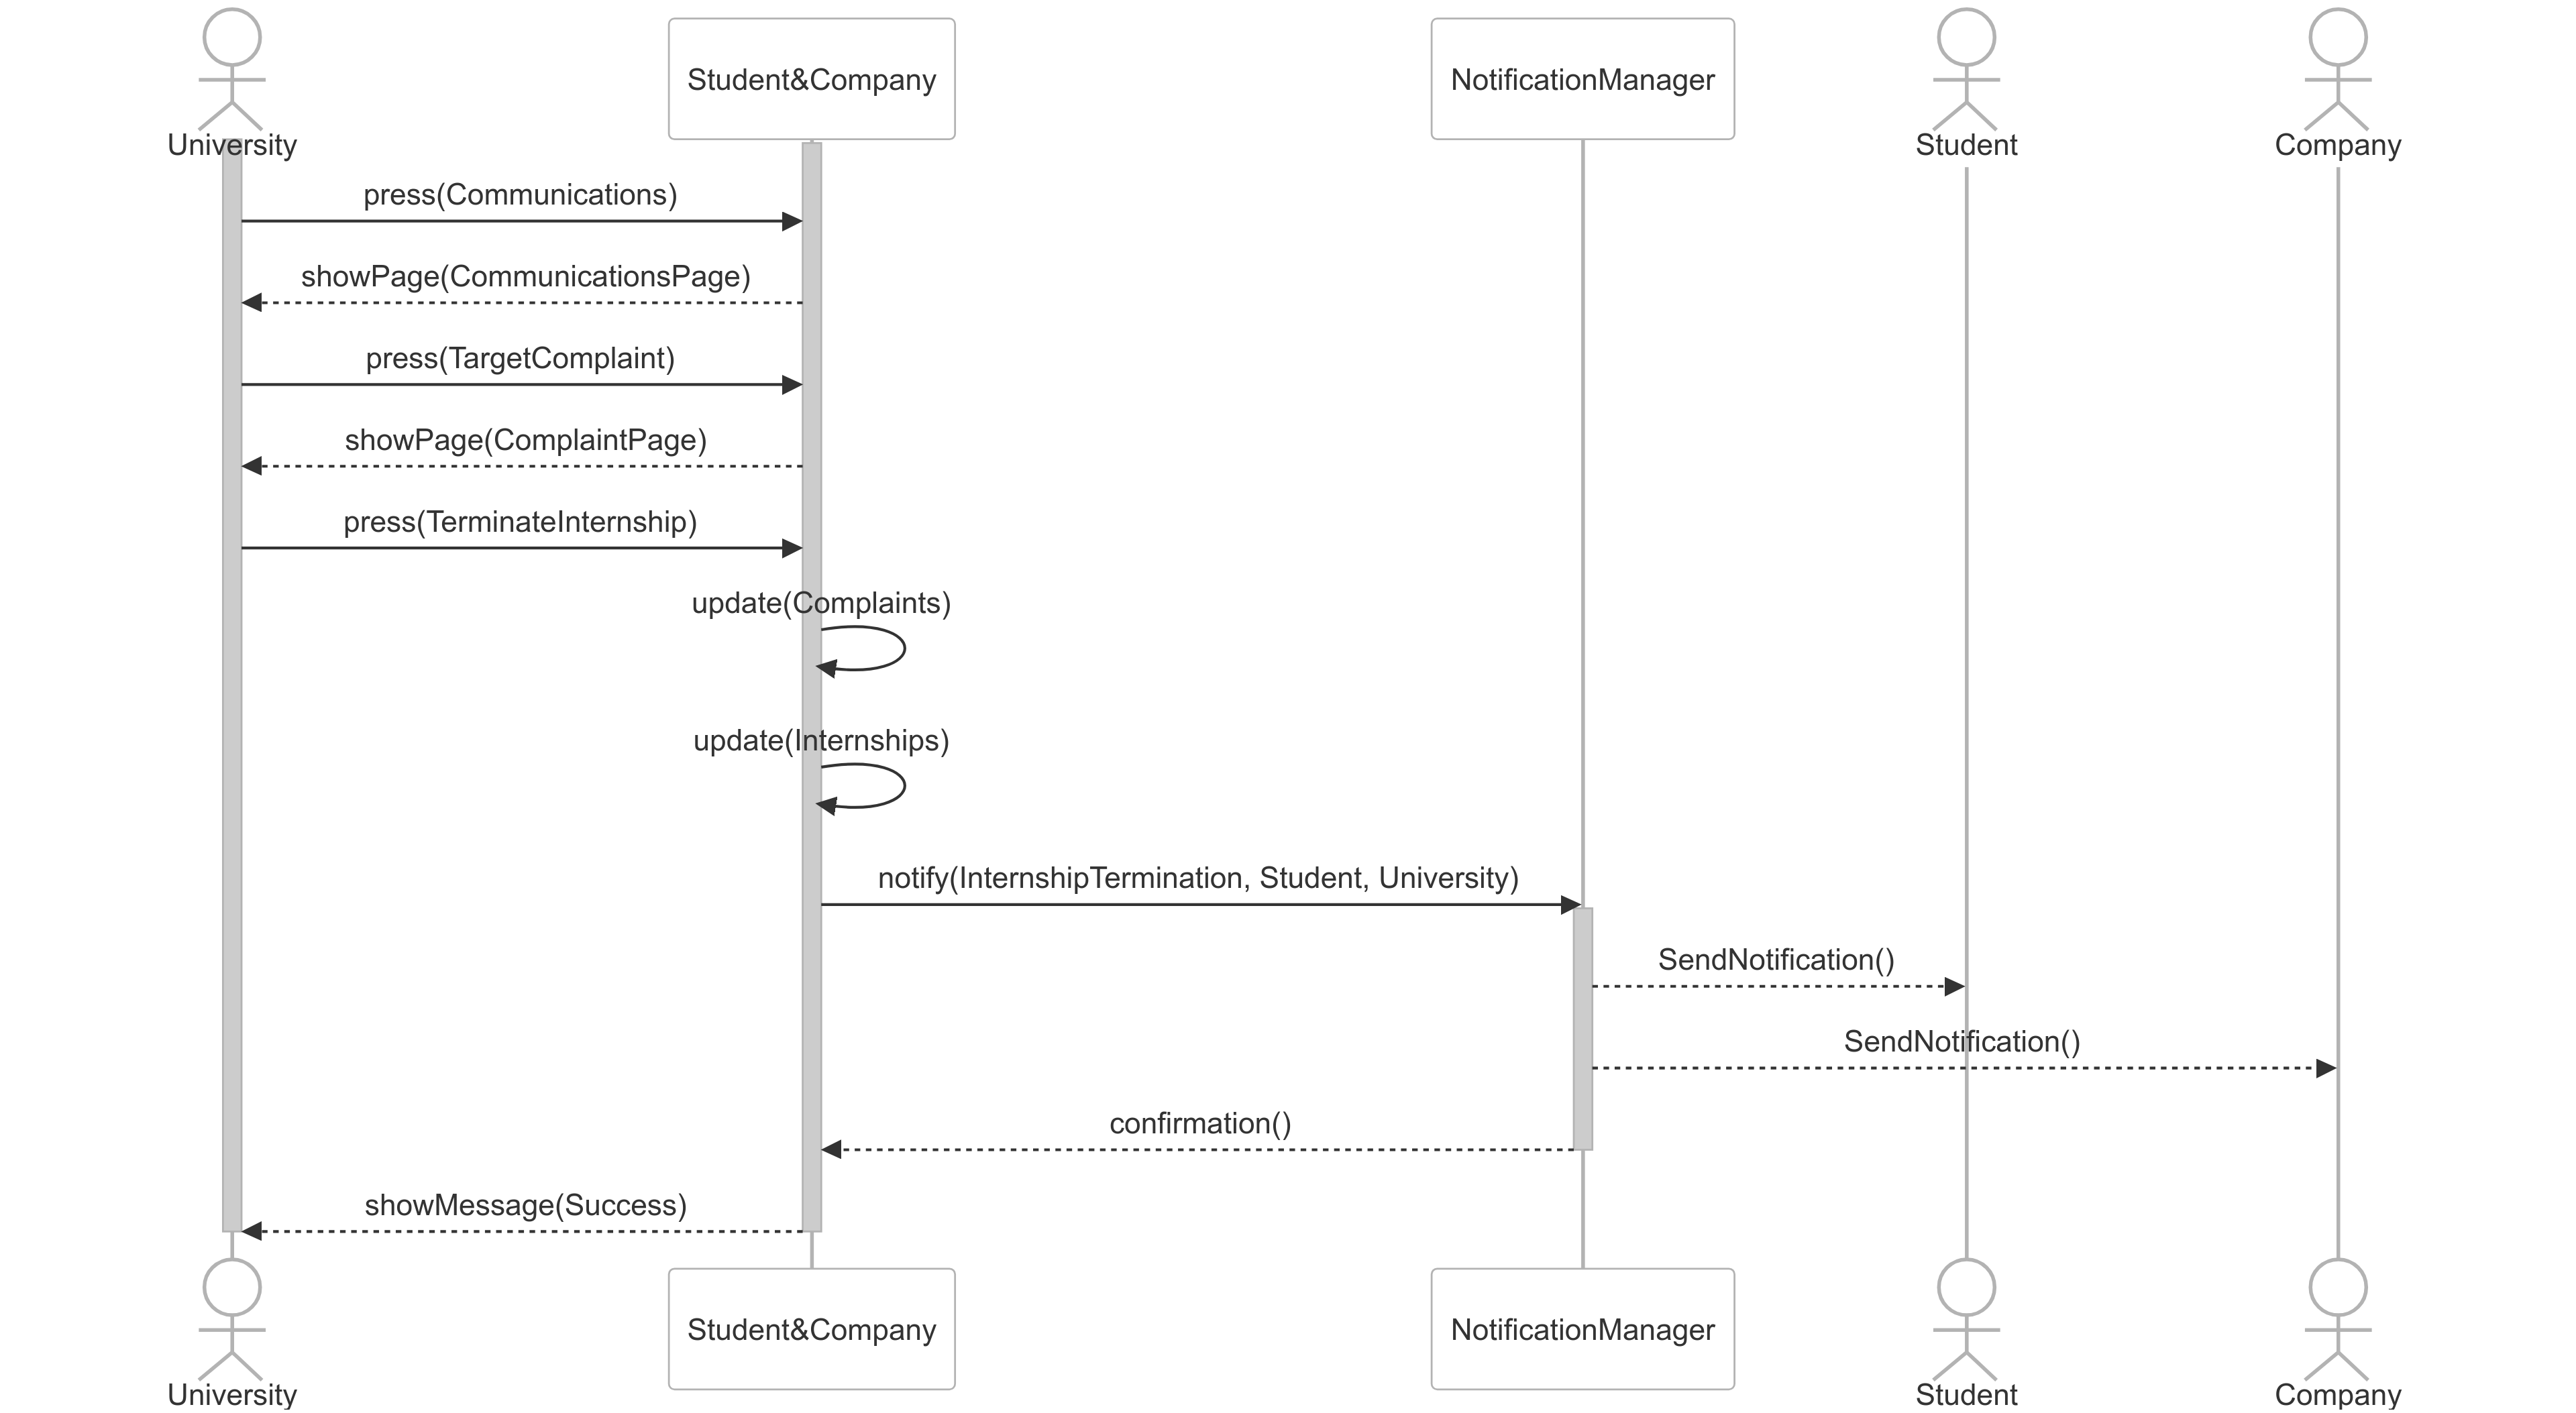
\includegraphics[width=1\textwidth]{Latex/Images/TerminateInternshipSequenceDiagram.png}
    \caption{[SD14]: Terminate Internship Sequence Diagram}
    \label{fig:SD14}
\end{figure}
\clearpage

\subsubsection{Requirements Mapping}

\begin{table}[H]
    \centering
    \begin{tabular}{|p{15cm}|}
         \hline
        \textbf{G1:} Companies would like to advertise the internships they offer. \\ \hline
        \begin{itemize}
            \item[\texttt{[D1]}] Students and Companies provide the Platform with correct and truthful information.
            \item[\texttt{[D2]}] Companies remove published Internship if they are no longer available.
            \item[\texttt{[D3]}] Students, Companies, and Universities receive every notification.
            \item[\texttt{[D4]}] Students, Companies, and Universities have a working internet connection.
        \end{itemize} \\ \hline
        \begin{itemize}
            \item[\texttt{[R1]}] The platform shall allow any unregistered students to register by providing personal information and selecting their University.
            \item[\texttt{[R2]}] The platform shall allow any companies to register by providing company information.
            \item[\texttt{[R3]}] The platform shall allow any universities to register by providing university information.
            \item[\texttt{[R4]}] The platform shall allow Users to log in using their email and password.
            \item[\texttt{[R5]}] The platform shall send notifications to Users when relevant events occur.
            \item[\texttt{[R6]}] The platform shall allow Companies to create and publish Internship offers specifying details.
            \item[\texttt{[R7]}] The platform shall allow Companies to terminate their Internship offers at their own discretion.
            \item[\texttt{[R9]}] The platform shall allow Students to view and navigate all available Internships.
        \end{itemize} \\ \hline
    \end{tabular}
    \caption{Goal 1 mapping}
    \label{tab:G1}
\end{table}
\clearpage
\begin{table}[H]
    \centering
    \begin{tabular}{|p{15cm}|}
         \hline
        \textbf{G2:} Students would like to autonomously candidate for available internships. \\ \hline
        \begin{itemize}
            \item[\texttt{[D1]}] Students and Companies provide the Platform with correct and truthful information. 
            \item[\texttt{[D2]}] Companies remove published Internship if they are no longer available.
            \item[\texttt{[D3]}] Students, Companies, and Universities receive every notification.
            \item[\texttt{[D4]}] Students, Companies, and Universities have a working internet connection.
        \end{itemize} \\ \hline
        \begin{itemize}
            \item[\texttt{[R1]}] The platform shall allow any unregistered students to register by providing personal information and selecting their University.
            \item[\texttt{[R2]}] The platform shall allow any companies to register by providing company information.
            \item[\texttt{[R3]}] The platform shall allow any universities to register by providing university information.
            \item[\texttt{[R4]}] The platform shall allow Users to log in using their email and password.
            \item[\texttt{[R5]}] The platform shall send notifications to Users when relevant events occur.
            \item[\texttt{[R6]}] The platform shall allow Companies to create and publish Internship offers specifying details.
            \item[\texttt{[R7]}] The platform shall allow Companies to terminate their Internship offers at their own discretion.
            \item[\texttt{[R9]}] The platform shall allow Students to view and navigate all available Internships.
            \item[\texttt{[R10]}] The platform shall enable Students to submit Spontaneous Applications to Internships they choose.
            \item[\texttt{[R13]}] The platform shall allow Students to monitor the status of their Spontaneous Applications.
            \item[\texttt{[R18]}] The platform shall allow Companies to accept a Spontaneous Application.
        \end{itemize} \\ \hline
    \end{tabular}
    \caption{Goal 2 mapping}
    \label{tab:G2}
\end{table}

\begin{table}[H]
    \centering
    \begin{tabular}{|p{15cm}|}
        \hline
        \textbf{G3:} Students would like to be matched with internships they might be interested in. \\ \hline
        \begin{itemize}
            \item[\texttt{[D1]}] Students and Companies provide the Platform with correct and truthful information.
            \item[\texttt{[D2]}] Companies remove published Internship if they are no longer available.
            \item[\texttt{[D3]}] Students, Companies, and Universities receive every notification.
            \item[\texttt{[D4]}] Students, Companies, and Universities have a working internet connection.
        \end{itemize} \\ \hline
        \begin{itemize}
            \item[\texttt{[R1]}] The platform shall allow any unregistered students to register by providing personal information and selecting their University.
            \item[\texttt{[R2]}] The platform shall allow any companies to register by providing company information.
            \item[\texttt{[R3]}] The platform shall allow any universities to register by providing university information.
            \item[\texttt{[R4]}] The platform shall allow Users to log in using their email and password.
            \item[\texttt{[R5]}] The platform shall send notifications to Users when relevant events occur.
            \item[\texttt{[R6]}] The platform shall allow Companies to create and publish Internship offers specifying details.
            \item[\texttt{[R7]}] The platform shall allow Companies to terminate their Internship offers at their own discretion.
            \item[\texttt{[R8]}] The platform shall provide Students with Matches automatically obtained by the Recommendation Process. 
            \item[\texttt{[R11]}] The platform shall allow Students to submit their CV.
            \item[\texttt{[R14]}] The platform shall allow Students to monitor the status of their Recommendation.
            \item[\texttt{[R15]}] The platform shall display to Students all the Internships found by the Recommendation Process.
            \item[\texttt{[R16]}] The platform shall display to Companies all the CVs of Matched Students obtained by the Recommendation Process.
            \item[\texttt{[R17]}] The platform shall allow Students and Companies to accept a Recommendation.
        \end{itemize} \\ \hline
    \end{tabular}
    \caption{Goal 3 mapping}
    \label{tab:G3}
\end{table}

\begin{table}[H]
    \centering
    \begin{tabular}{|p{15cm}|}
         \hline
        \textbf{G4:} Companies would like to perform interviews with suitable students. \\ \hline
        \begin{itemize}
            \item[\texttt{[D1]}] Students and Companies provide the Platform with correct and truthful information.
            \item[\texttt{[D2]}] Companies remove published Internship if they are no longer available.
            \item[\texttt{[D3]}] Students, Companies, and Universities receive every notification.
            \item[\texttt{[D4]}] Students, Companies, and Universities have a working internet connection.
        \end{itemize} \\ \hline
        \begin{itemize}
            \item[\texttt{[R1]}] The platform shall allow any unregistered students to register by providing personal information and selecting their University.
            \item[\texttt{[R2]}] The platform shall allow any companies to register by providing company information. 
            \item[\texttt{[R3]}] The platform shall allow any universities to register by providing university information.
            \item[\texttt{[R4]}] The platform shall allow Users to log in using their email and password.
            \item[\texttt{[R5]}] The platform shall send notifications to Users when relevant events occur.
            \item[\texttt{[R6]}] The platform shall allow Companies to create and publish Internship offers specifying details.
            \item[\texttt{[R17]}] The platform shall allow Students and Companies to accept a Recommendation.
            \item[\texttt{[R18]}] The platform shall allow Companies to accept a Spontaneous Application.
            \item[\texttt{[R19]}] The platform shall start a Selection Process only if both the Company and the Student have accepted the Recommendation.
            \item[\texttt{[R20]}] The platform shall start a Selection Process only if the Company has accepted the Spontaneous Application.
            \item[\texttt{[R21]}] The platform shall allow Companies to create Interviews.
            \item[\texttt{[R22]}] The platform shall allow Companies to submit Interviews to Students they have initiated a Selection Process with.
            \item[\texttt{[R23]}] The platform shall allow Students to answer Interview questions and submit them.
            \item[\texttt{[R24]}] The platform shall allow Companies to manually evaluate Interview submissions.
            \item[\texttt{[R25]}] The platform shall allow Students and Companies to monitor the status of their Interviews.
            \item[\texttt{[R26]}] The platform shall enable Companies to complete the Interview process by submitting the final outcome to each candidate.
        \end{itemize} \\ \hline
    \end{tabular}
    \caption{Goal 4 mapping}
    \label{tab:G4}
\end{table}

\begin{table}[H]
    \centering
    \begin{tabular}{|p{15cm}|}
        \hline
        \textbf{G5:} Students and companies would like to complain, communicate problems, provide information about an Ongoing Internship. \\ \hline
        \begin{itemize}
            \item[\texttt{[D1]}] Students and Companies provide the Platform with correct and truthful information.
            \item[\texttt{[D2]}] Companies remove published Internship if they are no longer available.
            \item[\texttt{[D3]}] Students, Companies, and Universities receive every notification.
            \item[\texttt{[D4]}] Students, Companies, and Universities have a working internet connection.
        \end{itemize} \\ \hline
        \begin{itemize}
            \item[\texttt{[R1]}] The platform shall allow any unregistered students to register by providing personal information and selecting their University.
            \item[\texttt{[R2]}] The platform shall allow any companies to register by providing company information.
            \item[\texttt{[R3]}] The platform shall allow any universities to register by providing university information.
            \item[\texttt{[R4]}] The platform shall allow Users to log in using their email and password.
            \item[\texttt{[R28]}] The platform shall enable Students to accept or reject an Internship Position Offer sent by a Company only if he previously passed the relative Interview.
            \item[\texttt{[R33]}] The platform shall provide a dedicated space for Students and Companies to exchange Communications about the current status of an Ongoing Internship.
        \end{itemize} \\ \hline
    \end{tabular}
    \caption{Goal 5 mapping}
    \label{tab:G5}
\end{table}

\begin{table}[H]
    \centering
    \begin{tabular}{|p{15cm}|}
        \hline
        \textbf{G6:} Students and companies would like to be provided with suggestions about how to improve their submission. \\ \hline
        \begin{itemize}
            \item[\texttt{[D1]}] Students and Companies provide the Platform with correct and truthful information.
            \item[\texttt{[D4]}] Students, Companies, and Universities have a working internet connection.
        \end{itemize} \\ \hline
        \begin{itemize}
            \item[\texttt{[R1]}] The platform shall allow any unregistered students to register by providing personal information and selecting their University.
            \item[\texttt{[R2]}] The platform shall allow any companies to register by providing company information.
            \item[\texttt{[R3]}] The platform shall allow any universities to register by providing university information.
            \item[\texttt{[R4]}] The platform shall allow Users to log in using their email and password.
            \item[\texttt{[R6]}] The platform shall allow Companies to create and publish Internship offers specifying details.
            \item[\texttt{[R7]}] The platform shall allow Companies to terminate their Internship offers at their own discretion.
            \item[\texttt{[R12]}] The platform shall allow Students to modify their CV.
            \item[\texttt{[R29]}] The platform shall collect Feedback from both Students and Companies regarding the Recommendation Process.
            \item[\texttt{[R30]}] The platform shall provide Suggestions to Students on improving their CVs.
            \item[\texttt{[R31]}] The platform shall provide Suggestions to Companies on improving Internship descriptions.
        \end{itemize} \\ \hline
    \end{tabular}
    \caption{Goal 6 mapping}
    \label{tab:G6}
\end{table}

\begin{table}[H]
    \centering
    \begin{tabular}{|p{15cm}|}
        \hline
        \textbf{G7:} Universities would like to handle complains about Ongoing Internships. \\ \hline
        \begin{itemize}
            \item[\texttt{[D1]}] Students and Companies provide the Platform with correct and truthful information.
            \item[\texttt{[D2]}] Companies remove published Internship if they are no longer available. 
            \item[\texttt{[D3]}] Students, Companies, and Universities receive every notification.
            \item[\texttt{[D4]}] Students, Companies, and Universities have a working internet connection.
            \item[\texttt{[D5]}] Universities interrupt an Ongoing Internship only if no solution to complaints are found.
        \end{itemize} \\ \hline
        \begin{itemize}
            \item[\texttt{[R1]}] The platform shall allow any unregistered students to register by providing personal information and selecting their University.
            \item[\texttt{[R2]}] The platform shall allow any companies to register by providing company information.
            \item[\texttt{[R3]}] The platform shall allow any universities to register by providing university information.
            \item[\texttt{[R4]}] The platform shall allow Users to log in using their email and password.
            \item[\texttt{[R5]}] The platform shall send notifications to Users when relevant events occur.
            \item[\texttt{[R32]}] The platform shall allow registered Universities to access and monitor Internship Communications related to their Students.
            \item[\texttt{[R33]}] The platform shall provide a dedicated space for Students and Companies to exchange Communications about the current status of an ongoing Internship.
            \item[\texttt{[R34]}] The platform shall allow registered Universities to handle Complaints and to interrupt an Internship at their own discretion.
        \end{itemize} \\ \hline
    \end{tabular}
    \caption{Goal 7 mapping}
    \label{tab:G7}
\end{table}


\begin{table}[H]
    \centering
    \begin{tabular}{|p{15cm}|}
        \hline
        \textbf{G8:} Students would like to choose which internship to attend from among those for which they passed the interview. \\ \hline
        \begin{itemize}
            \item[\texttt{[D1]}] Students and Companies provide the Platform with correct and truthful information.
            \item[\texttt{[D2]}] Companies remove published Internship if they are no longer available. 
            \item[\texttt{[D4]}] Students, Companies, and Universities have a working internet connection.
        \end{itemize} \\ \hline
        \begin{itemize}
            \item[\texttt{[R1]}] The platform shall allow any unregistered students to register by providing personal information and selecting their University.
            \item[\texttt{[R2]}] The platform shall allow any companies to register by providing company information.
            \item[\texttt{[R3]}] The platform shall allow any universities to register by providing university information.
            \item[\texttt{[R4]}] The platform shall allow Users to log in using their email and password.
            \item[\texttt{[R6]}] The platform shall allow Companies to create and publish Internship offers specifying details.
            \item[\texttt{[R7]}] The platform shall allow Companies to terminate their Internship offers at their own discretion.
            \item[\texttt{[R17]}] The platform shall allow Students and Companies to accept a Recommendation.
            \item[\texttt{[R18]}] The platform shall allow Companies to accept a Spontaneous Application.
            \item[\texttt{[R22]}] The platform shall allow Companies to submit Interviews to Students they have initiated a Selection Process with.
            \item[\texttt{[R23]}] The platform shall allow Students to answer Interview questions and submit them.
            \item[\texttt{[R26]}] The platform shall enable Companies to complete the Interview process by submitting the final outcome to each candidate.
            \item[\texttt{[R28]}] he platform shall enable Students to accept or reject an Internship Position Offer sent by a Company only if he previously passed the relative Interview.
        \end{itemize} \\ \hline
    \end{tabular}
    \caption{Goal 8 mapping}
    \label{tab:G8}
\end{table}


\begin{table}[H]
    \centering
    \begin{tabular}{|p{15cm}|}
        \hline
        \textbf{G9:} Companies would like to select students for the internship position among those who passed the interview. \\ \hline
        \begin{itemize}
            \item[\texttt{[D1]}] Students and Companies provide the Platform with correct and truthful information.
            \item[\texttt{[D2]}] Companies remove published Internship if they are no longer available. 
            \item[\texttt{[D4]}] Students, Companies, and Universities have a working internet connection.
        \end{itemize} \\ \hline
        \begin{itemize}
            \item[\texttt{[R1]}] The platform shall allow any unregistered students to register by providing personal information and selecting their University.
            \item[\texttt{[R2]}] The platform shall allow any companies to register by providing company information.
            \item[\texttt{[R3]}] The platform shall allow any universities to register by providing university information.
            \item[\texttt{[R4]}] The platform shall allow Users to log in using their email and password.
            \item[\texttt{[R6]}] The platform shall allow Companies to create and publish Internship offers specifying details.
            \item[\texttt{[R7]}] The platform shall allow Companies to terminate their Internship offers at their own discretion.
            \item[\texttt{[R17]}] The platform shall allow Students and Companies to accept a Recommendation.
            \item[\texttt{[R18]}] The platform shall allow Companies to accept a Spontaneous Application.
            \item[\texttt{[R22]}] The platform shall allow Companies to submit Interviews to Students they have initiated a Selection Process with.
            \item[\texttt{[R23]}] The platform shall allow Students to answer Interview questions and submit them.
            \item[\texttt{[R26]}] The platform shall enable Companies to complete the Interview process by submitting the final outcome to each candidate.
            \item[\texttt{[R27]}] The platform shall enable Companies to send an Internship Position Offer to a Student only if he previously passed the relative Interview.
        \end{itemize} \\ \hline
    \end{tabular}
    \caption{Goal 9 mapping}
    \label{tab:G9}
\end{table}


\begin{table}[H]
    \centering
    \begin{tabular}{|c|c|c|c|c|c|c|c|c|c|}
        \hline &   
        \textbf{G1} & 
        \textbf{G2} & 
        \textbf{G3} & 
        \textbf{G4} & 
        \textbf{G5} & 
        \textbf{G6} & 
        \textbf{G7} & 
        \textbf{G8} & 
        \textbf{G9} \\ \hline
        %              1   2   3   4   5   6   7   8   9
        \textbf{D1}  & x & x & x & x & x & x & x & x & x \\ \hline
        \textbf{D2}  & x & x & x & x & x &   & x & x & x \\ \hline
        \textbf{D3}  & x & x & x & x & x &   & x &   &   \\ \hline
        \textbf{D4}  & x & x & x & x & x & x & x & x & x \\ \hline
        \textbf{D5}  &   &   &   &   &   &   & x &   &   \\ \hline\hline
        \textbf{R1}  & x & x & x & x & x & x & x & x & x \\ \hline
        \textbf{R2}  & x & x & x & x & x & x & x & x & x \\ \hline
        \textbf{R3}  & x & x & x & x & x & x & x & x & x \\ \hline
        \textbf{R4}  & x & x & x & x & x & x & x & x & x \\ \hline
        \textbf{R5}  & x & x & x & x & x &   & x &   &   \\ \hline
        \textbf{R6}  & x & x & x & x &   & x &   & x & x \\ \hline
        \textbf{R7}  & x & x & x &   &   & x &   & x & x \\ \hline
        \textbf{R8}  &   &   & x &   &   &   &   &   &   \\ \hline
        \textbf{R9}  & x & x &   &   &   &   &   &   &   \\ \hline
        \textbf{R10} &   & x &   &   &   &   &   &   &   \\ \hline
        \textbf{R11} &   &   & x &   &   &   &   &   &   \\ \hline
        \textbf{R12} &   &   &   &   &   & x &   &   &   \\ \hline
        \textbf{R13} &   & x &   &   &   &   &   &   &   \\ \hline
        \textbf{R14} &   &   & x &   &   &   &   &   &   \\ \hline
        \textbf{R15} &   &   & x &   &   &   &   &   &   \\ \hline
        \textbf{R16} &   &   & x &   &   &   &   &   &   \\ \hline
        \textbf{R17} &   &   & x & x &   &   &   & x & x \\ \hline
        \textbf{R18} &   & x &   & x &   &   &   & x & x \\ \hline
        \textbf{R19} &   &   &   & x &   &   &   &   &   \\ \hline
        \textbf{R20} &   &   &   & x &   &   &   &   &   \\ \hline
        \textbf{R21} &   &   &   & x &   &   &   &   &   \\ \hline
        \textbf{R22} &   &   &   & x &   &   &   & x & x \\ \hline
        \textbf{R23} &   &   &   & x &   &   &   & x & x \\ \hline
        \textbf{R24} &   &   &   & x &   &   &   &   &   \\ \hline
        \textbf{R25} &   &   &   & x &   &   &   &   &   \\ \hline
        \textbf{R26} &   &   &   & x &   &   &   & x & x \\ \hline
        \textbf{R27} &   &   &   &   &   &   &   &   & x \\ \hline
        \textbf{R28} &   &   &   &   & x &   &   & x &   \\ \hline
        \textbf{R29} &   &   &   &   &   & x &   &   &   \\ \hline
        \textbf{R30} &   &   &   &   &   & x &   &   &   \\ \hline
        \textbf{R31} &   &   &   &   &   & x &   &   &   \\ \hline
        \textbf{R32} &   &   &   &   &   &   & x &   &   \\ \hline
        \textbf{R33} &   &   &   &   & x &   & x &   &   \\ \hline
        \textbf{R34} &   &   &   &   &   &   & x &   &   \\ \hline
    \end{tabular}
    \caption{Goals and Requirements Mapping Table}
    \label{tab:requirements_mapping}
\end{table}
\clearpage 
\subsection{Performance Requirements}
 Given the system's non-critical nature, stringent performance criteria are unnecessary. However, to ensure an optimal User experience:
\begin{itemize}
  \item The system shall notify Users within 2 seconds after an event has occurred
  \item The system shall respond to User requests within 2 seconds under normal load conditions
  \item The system shall support at least 1000 concurrent Users
  \item Database queries shall be completed within 1.5 seconds
  \item The system shall handle up to 10,000 internship listings simultaneously
  \item The system shall support up to 100,000 registered Users
  \item The system shall support up to 1000 registered Companies
  \item The system shall support up to 100 registered Universities
  \item The Recommendation Process shall be completed within 300 seconds under normal load conditions
  \item The Suggestions computed by the platform shall be provided to the User within 180 seconds after the CV or the Internship Offer has been submitted
\end{itemize}
\subsection{Design Constraints}
This section explain the different constraints that the platform must respect such as the standard compliance for the data protection and hardware limitations.
\subsubsection{Standards Compliance}
Student\&Company will handle and process highly sensitive data, including but not limited to personal information, Student's CVs and proprietary information of Company and University.\\
Because of that the Platform must not only be able to comply with the General Data Protection Regulation (GDPR) and any other Data/Privacy Law present in the countries where the Platform will be used (e.g California Consumer Privacy Act "CCPA" or similar law), but also have to be flexible enough to adopt custom policies set by Companies and Universities to protect their data and the data of their own users.
\subsubsection{Hardware limitations}
The platform is a web application that can be accessed from any device with a web browser and an internet connection. No special hardware is required a part from a device with a network card
\subsection{Software System Attributes}
This section provides an overview of the system's key attributes such as reliability and availability, security, maintainability, and portability explained in a technical and non-technical way.
\subsubsection{Reliability \& Availability}
The platform is designed to be highly reliable and available to Users, with a target uptime of at lest 99.862\%. This means that the system should be unreachable for Users for no more than 12 hours in a year. To achieve this, the platform will be hosted on redundant servers with automatic failover capabilities and a load balancer to distribute traffic evenly between the different machines. \\
Furthermore, to ensure the availability of the platform, scheduled maintenance will be schedule during low traffic days such as during winter or summer break.\\
This approach is intended to guarantee that the system remains fully operational at the start of each semester, when the traffic expected to be much higher due to the increase in the number of Students and Companies looking for Internships.\\
\subsubsection{Security}
Due to the highly sensitive nature of the data processed by the platform, security is a top priority for S\&C. We will implement a multi-layered security approach to protect the data of our Users such as:
\begin{itemize}
  \item The use of HTTPS protocol to encrypt data exchanged between the User and the Platform
  \item Strong password requirements and email verification for all users
  \item Failed login attempts shall be limited to 5 before temporary account lockout
  \item Password encryption using industry-standard hashing algorithms such as MD5 or SHA-256
  \item Role-based access control to ensure that Users can only access the data they are authorized to see
  \item Verification of Companies and Universities profile will be conducted using their VAT numbers, once the official governance API becomes available.
\end{itemize}

\subsubsection{Maintainability}
The system should be designed to be easily maintainable and scalable to accommodate future growth. This includes the use of modular code, clear documentation, and a well-defined architecture that allows for easy updates and modifications both on the front and the back end. \\
The platform should also be designed to be easily scalable to accommodate an increase in the number of Users and Internship Offers and in a way where the need of adding new features or fixing bugs should not require a complete overhaul of the system.\\
\subsubsection{Portability}
As a web application, the platform is inherently portable by design, allowing access from any device equipped with a web browser and an internet connection. There are no additional portable constraints on the server-side infrastructure of the platform.